\documentclass{tietreport}

% Import images
\usepackage{graphicx}
\usepackage{array}
\usepackage{enumitem}
\usepackage{rotating}
\usepackage{microtype}
\usepackage{longtable}
\usepackage{float}
% Let pages end short rather than stretching the space between paragraphs, which
% left large gaps next to the long tables and figure pages.
\raggedbottom

% Plain links: the boxes hyperref draws by default do not survive printing well.
\hypersetup{hidelinks}

% The class sets a 12pt header but leaves \headheight at its 12pt default, which makes
% fancyhdr warn on every page. Give it the 14.5pt it asks for.
\setlength{\headheight}{14.5pt}

% The blank verso the class inserts before each chapter should not carry a running
% header; without this it looks like a page that failed to typeset.
\makeatletter
\renewcommand{\cleardoublepage}{%
  \clearpage
  \if@twoside
    \ifodd\c@page\else
      \hbox{}\thispagestyle{empty}\newpage
    \fi
  \fi}
\makeatother

% The text block here is narrow and the prose carries long snake_case identifiers.
% A little emergency stretch keeps paragraphs inside the margin without \sloppy
% ruining the spacing everywhere.
\setlength{\emergencystretch}{3em}


% Bibliography configuration
\usepackage[
  date=year,
  style=alphabetic,
  backend=biber,
  sorting=nty,
  maxnames=5,
  minnames=3,
  maxalphanames=4,
  minalphanames=3,
  backref=true,
  doi=false,
  isbn=false,
  url=false,
  eprint=false
]{biblatex}
\addbibresource{references.bib}
% Let biblatex break long URLs rather than run them into the margin.
\setcounter{biburlnumpenalty}{9000}
\setcounter{biburlucpenalty}{9000}
\setcounter{biburllcpenalty}{9000}


% A narrow fixed-width column that wraps, used by the tables in Chapters 2 and 4.
\newcolumntype{L}[1]{>{\raggedright\arraybackslash}p{#1}}

%% ==================================================
%% CUSTOMIZE THESE FIELDS FOR YOUR PROJECT
%% ==================================================

% Course/Lab header
\TitlePageHeader{%
  UCS503P - Software Engineering Project (2026-27 ODD)%
}

% Main project title
\ProjectTitle{%
  Campus Companion%
}

% Subtitle or project description
\ProjectSubTitle{%
  Finding Someone to Go With: Host-Approved Activity Matching
  for Thapar Students%
}

% Student information (up to 4 students)
% Set as a two-column table rather than four separate lines: the class centres
% each line of the author block on its own, so lines of different width start at
% different points and the roll numbers never form a column.
\author{%
  \begin{tabular}{@{}r@{\hspace{0.65em}}l@{}}
    \texttt{1024030549} & Aryan Vasdev \\
    \texttt{1024030551} & Shraney Sharma \\
    \texttt{1024030553} & Ishaan Sharma \\
    \texttt{1024030554} & Saumya Singh
  \end{tabular}%
}

% Group number, degree, year, program
\TitlePageSubText{%
  Group: \texttt{3C42} BE Third Year, CSE%
}

% Faculty advisor/guide name
\AdvisorName{%
  Ms. Reaya Grewal%
}

% Evaluation period and department info
\TitlePageFooterText{{%
    \large End-Semester Evaluation (Final Report) \\[0.2cm]
    \bfseries Computer Science and Engineering
    Department%
  } \\[0.15cm]
  Thapar Institute of Engineering and Technology,
  Patiala%
}

%% ==================================================

\begin{document}

\maketitle

\tableofcontents


% ===== CHAPTER 1: INTRODUCTION =====

\chapter{Introduction}

\section{Background and Context}

A residential campus is unusual in that almost everything a student might want
to do is within walking distance and almost everyone who might want to do it is
within walking distance too. What is missing is the introduction. A student who
wants to walk to the lake on a Sunday morning, find a fourth for badminton, or
simply not eat dinner alone is rarely blocked by the activity itself. They are
blocked by not knowing who else is free, and by the small social cost of asking.

The channels that exist today were not built for this. Class and hostel WhatsApp
groups carry a plan for the ten minutes before it scrolls away; nobody can find it
afterwards, nobody knows who actually turned up, and a message sent to two hundred
people to find three is mostly noise. Instagram stories reach an audience selected
by who already follows whom, which is exactly the wrong filter for a first-year
student or a transfer who has not built that network yet. Neither channel gives the
person proposing the plan any control over who shows up, and neither leaves any
record afterwards.

\emph{Campus Companion} is a mobile application for students of Thapar Institute
of Engineering and Technology that turns this into a small, explicit workflow.
A student posts an activity with a place, a time, a duration and a head count. Other
students find it, and ask to join. The person who posted it decides who is in.
Once the activity is over, the people who were there rate each other, and that
rating follows them to the next listing. The guiding idea is that a plan between
students who do not already know each other needs three things the group chat
cannot provide: \textbf{admission control, a record, and a safety net}.

\subsection{Why matching, and not another social network}

The project deliberately does not build profiles, feeds, follows or discovery of
people. The unit of the product is an \emph{activity}, not a person. A student
never browses other students; they browse things happening, and the only way to
reach another student is through an activity that both of them are in, or through
a direct conversation opened from one. This keeps the product narrow enough to
finish in a semester, and it removes the whole class of problems that come with
letting anyone message anyone.

\subsection{Why safety is a first-class requirement}

The honest description of the product is that it asks students to meet people they
do not know, in a physical place, at a stated time. That is the value, and it is
also the risk. Three design decisions follow directly from it and are present in
the code from the first week rather than bolted on:

\begin{itemize}[nosep]
  \item Only an \texttt{@thapar.edu} address can hold an account, and that address
        must be proven by a one-time code before the account can be used at all.
        Everybody on the platform is verifiably a member of the institute.
  \item Joining is a request, not an action. The host sees who is asking, together
        with their average rating, and admits them one at a time.
  \item Every account can store an emergency contact, and the server can send that
        contact a text message carrying the student's live coordinates and the names
        of the people they are currently out with.
\end{itemize}

\section{Problem Statement}

Four specific problems were identified before any code was written, and each one is
answered by a named part of the system:

\begin{itemize}
  \item \textbf{Plans are invisible and perishable.} A proposal made in a chat group
        is discoverable only by the people looking at their phone in that minute.
        There is no way to search for what is happening on Saturday afternoon.

  \item \textbf{There is no admission control.} Anyone in a group of two hundred can
        say they are coming. The student who proposed the plan has no mechanism to
        say no, and in practice will not say it socially in front of the group.

  \item \textbf{Nothing is remembered.} Whether somebody turned up, was pleasant, or
        cancelled at the last minute is known to the four people who were there and
        to nobody else. The same mistake is available to be repeated indefinitely.

  \item \textbf{There is no safety net.} A student going to meet people they met
        online has told no system where they are going, when, or with whom. If
        something goes wrong there is nothing to hand to anyone.
\end{itemize}

\noindent\textbf{Why this is worth solving now.} The cost of the status quo is not
dramatic; it is that a large number of students do slightly less than they would
like to, slightly more alone than they would like to be. The institute already has
the two ingredients that make a solution tractable, namely a captive population in
a small geography and a single authoritative e-mail domain. A modest tool that
lowers the cost of one introduction, repeated across a campus, is a reasonable
thing to build.

\section{Project Objectives}

The objectives are written so that each can be checked at this evaluation and again
at the end of the semester.

\begin{enumerate}
  \item \textbf{Institution-restricted, verified identity (complete).} Allow only
        \texttt{@thapar.edu} addresses to register, prove each address with a
        time-limited one-time code before the account may be used, and provide a
        password reset path that runs on the same mechanism without ever revealing
        whether an address is registered. Since the mid-semester evaluation a student
        can also check their account against their physical Thapar ID card, which
        earns a red tick shown beside their name.

  \item \textbf{A complete hosting and joining workflow (complete).} Let a student
        publish an activity with category, time, duration, capacity and landmark;
        let other students browse and filter what is on; and settle every join
        through an explicit request that the host accepts or declines, with capacity
        enforced correctly under concurrent taps.

  \item \textbf{Private group communication per activity (complete).} Give every
        activity a conversation that exists from the moment it is created, admit a
        student to it at the instant their request is accepted, and deliver messages
        over a persistent connection rather than by polling.

  \item \textbf{A reputation signal that is earned, not claimed (complete).} Allow
        participants of a finished activity to rate one another once each, hold the
        score to a half-star scale, refuse ratings before the activity has ended, and
        show the resulting average wherever a student's activity appears.

  \item \textbf{A safety path from the app to a real person (partially complete).}
        Store an emergency contact per account and, on an SOS, text that contact the
        student's coordinates as a map link together with the names of the companions
        they are currently out with. The server side of this is finished and tested.
        The button in the application still shows a ``coming soon'' message, so this
        objective is not met at the final evaluation. Chapter~\ref{ch:conclusion}
        explains why.

  \item \textbf{Measurable outcomes rather than anecdote (instrumented; pilot not
        run).} Record enough timestamps that time-to-a-confirmed-companion,
        acceptance rate and fill rate can be computed from the database rather than
        estimated. The columns exist and are written. The two-week pilot did not
        happen, so Chapter~\ref{ch:results} reports measurements of the system
        itself (response times, scaling, test results) instead of usage figures.
\end{enumerate}

\section{Scope of this Report}

This is the final report. It keeps the mid-semester report as its base and adds what
was built and tested after it. Every figure and number in it was produced from the code
in the project repository~\cite{campuscompanion2026}, which is public at
\url{https://github.com/aryanvasdev-th/ucs503p-202627companionfinder} (the app is
under \texttt{code/frontend} and the server under \texttt{code/backend}).

Chapter~2 records the feasibility study and where the build departed from it.
Chapter~3 describes the architecture and walks through each module, including the
seven added since mid-semester. Chapter~4 sets out the evaluation criteria and where the
project stands against the six objectives. Chapter~5 covers testing: the test plan,
all 48 automated test cases with their results, and screenshots of the application
for each user-facing case. Chapter~6 analyses the system with measured response times,
scaling behaviour and code growth. Chapter~7 holds the UML models, now including
sequence, communication, state, component and deployment diagrams. Chapter~8 concludes,
and Chapter~9 is the project journal, recording who did what and when.


% ===== CHAPTER 2: FEASIBILITY STUDY =====

\chapter{Feasibility Study}

This chapter reproduces the feasibility study carried out before implementation
began. It covers the standard technical, managerial, economic, financial, cultural,
social, safety and political dimensions~\cite{sommerville2016,pressman2020}.
Section~\ref{sec:divergence} records where the system described in Chapter~\ref{ch:design}
has since departed from what was proposed here.

\section{Go / No-Go Decision}

\noindent\textbf{Decision: GO.}

The proposed Campus Companion application is technically achievable with currently
available technologies and the skills that can be developed by the four-member project
team. The project has a clear target audience --- college students --- and addresses
practical problems such as making daily activities more feasible by finding companions,
coordinating schedules, building trust among users, and improving personal safety.

The complete feature set is ambitious, particularly the personality-based match-making,
facial verification, and SOS functionality. However, the project can be implemented
incrementally, with essential coordination features forming the core system and the more
advanced features being added in the later stages.

\section{Technical Feasibility}

All major components of this project can be implemented using already established
software technology.

The Frontend can be developed as a mobile application using Flutter and Dart while the
backend can be developed using Node.js/Express.js or any other equivalent backend
framework. PostgreSQL/Firebase can be used for storing user profiles, activities,
ratings, preferences, and participation data.

The application's real-time features, such as live participant counters and waiting
period countdowns, can be implemented using Firebase/WebSockets. Recurring activities can
be handled using scheduled backend tasks.

The personality compatibility system can be developed using Python, NumPy, Pandas and
Scikit-learn, using user questionnaire responses as feature vectors and applying
similarity or clustering algorithms to generate compatibility scores.

The webcam-based identity verification feature can be implemented using Python, OpenCV
and face-recognition/deep-learning models. Since this is comparatively complex, a basic
face-verification prototype can be implemented for the project rather than a
production-grade biometric authentication system.

The SOS functionality requires access to device location services and communication APIs.
The application can transmit the user's current location and details of the ongoing
interaction to a pre-registered local emergency contact.

Therefore, the required technologies are available and suitable for the project. The
principal technical challenge is not the availability of technology but integrating the
different components reliably and securely.

\noindent\textbf{Assessment: Highly feasible}

\section{Managerial Feasibility}

The project is being developed by a four-member team, allowing responsibilities to be
divided according to technical domains. The project can be divided into four major areas:

\begin{itemize}[nosep]
  \item Frontend and Machine Learning: user interface, activity feed, profile system and
        compatibility algorithm.
  \item Backend: APIs, authentication, activity management, scheduling and business logic.
  \item Database and Real-Time Systems: database architecture, participant tracking,
        real-time updates and cloud storage.
  \item Computer Vision, Testing and Deployment: face verification, testing, deployment
        and software integration.
\end{itemize}

This division allows team members to learn their respective technologies in parallel
while maintaining clear ownership of individual modules.

Version control using Git/GitHub and a modular architecture will allow the four members
to work independently and integrate their modules later.

The project does not require a large organizational infrastructure because the proposed
system is primarily software-based and can initially be deployed for a single college
campus.

\noindent\textbf{Assessment: Feasible}

\section{Economic Feasibility}

The project has relatively low development costs because most of the required
technologies and frameworks are open-source or provide free/student-level usage.

The primary costs would potentially arise from:

\begin{itemize}[nosep]
  \item Cloud database and server usage as the number of users increases.
  \item Storage of profile images and other media.
  \item SMS/communication APIs for emergency notifications.
  \item Maps and location-based services.
  \item Hosting and deployment.
\end{itemize}

For an academic prototype limited to a college campus, these costs can be minimized
through free tiers and local development environments.

From a potential product perspective, the application may provide economic benefits by
creating a scalable platform that can later be expanded to multiple campuses. Possible
future revenue models could include premium campus services, partnerships with colleges
or student organizations, and sponsored campus activities.

Since the current objective is an academic project rather than immediate
commercialization, the expected development cost is low relative to the potential
functional value demonstrated by the system.

\noindent\textbf{Assessment: Feasible}

\section{Financial Feasibility}

The project does not require significant initial capital because development can be
carried out using existing personal computers, open-source software, free development
frameworks and cloud free tiers.

The main financial requirement is the cost of hosting and third-party services if the
application moves beyond a prototype. These costs can initially be kept low by
restricting deployment to a single campus and a limited number of users.

The project also does not require physical infrastructure, manufacturing, transportation
or inventory. This considerably reduces financial risk.

For a future production deployment, additional funding would be required for scalable
cloud infrastructure, security, maintenance, legal compliance and potentially dedicated
emergency communication services.

\noindent\textbf{Assessment: Feasible for an academic prototype; moderate financial
requirements for large-scale deployment.}

\section{Cultural Feasibility}

The application is designed specifically for college students and fits naturally into the
social and collaborative culture of a university campus.

Students commonly participate in activities such as:

\begin{itemize}[nosep]
  \item Gym and sports
  \item Clubs and societies
  \item Study sessions
  \item Events and workshops
  \item Gaming
  \item Food and recreational activities
\end{itemize}

The use of a casual, modern and Gen-Z-oriented interface is also compatible with the
target demographic. Features such as personality compatibility and informal review
prompts are intended to make interaction more approachable than conventional
event-management applications.

However, cultural differences in social preferences, gender interactions, privacy
expectations and willingness to meet unfamiliar people must be considered during
development.

The application should therefore provide users with control over preferences and
visibility rather than forcing them into social interactions.

\noindent\textbf{Assessment: Feasible}

\section{Social Feasibility}

The application has significant potential social benefits because it can reduce the
difficulty of finding people to participate in activities with.

It can help students:

\begin{itemize}[nosep]
  \item Meet people with similar interests.
  \item Participate in activities they might otherwise avoid.
  \item Coordinate activities more efficiently.
  \item Build new social connections.
  \item Find companions for routine activities.
  \item Reduce the inconvenience of repeatedly organizing the same activity.
\end{itemize}

The compatibility system and reliability ratings can further help users make informed
decisions before interacting with unfamiliar students.

However, the social nature of the platform also introduces risks such as harassment,
inappropriate behavior, discrimination, fake profiles and misuse of ratings. A reporting
mechanism, moderation process, privacy controls and user blocking functionality should
therefore be incorporated into the design.

\noindent\textbf{Assessment: Feasible with appropriate moderation and privacy controls.}

\section{Safety Feasibility}

Safety is a major consideration because the application involves interactions between
potentially unfamiliar students.

The proposed safety mechanisms include:

\begin{itemize}[nosep]
  \item User verification.
  \item Reliability scores and reviews.
  \item Reporting of inappropriate behavior.
  \item Gender-based activity preferences.
  \item An SOS mechanism.
  \item Sharing of current location during emergencies.
  \item Information about the person with whom the user is interacting.
\end{itemize}

These features can significantly improve user confidence. However, safety-related
functionality must not be presented as a guarantee that a user is safe. For example,
webcam verification can establish a degree of identity confidence but cannot completely
prevent harmful behavior.

The SOS feature must also be designed carefully because incorrect location information,
network failure, unavailable APIs or device permission restrictions could affect its
operation. Emergency functionality should therefore be tested thoroughly and clearly
communicate its limitations.

Privacy and secure handling of location, biometric and personal information are
essential.

\noindent\textbf{Assessment: Feasible but requires high attention to privacy, security
and reliability.}

\section{Political Feasibility}

The application does not have significant political dependencies for deployment as an
academic prototype. However, deployment within an actual college campus may require
permission from the institution and compliance with the college's policies regarding
student data, location tracking, photographs, communication and emergency services.

The application would also need to follow applicable data-protection and privacy
requirements, particularly because it may process sensitive information such as profile
photographs, location data, emergency contacts and biometric verification data.

For the academic prototype, these concerns can be addressed by limiting the user base,
obtaining user consent, clearly defining the data collected, and implementing appropriate
access controls.

\noindent\textbf{Assessment: Feasible, subject to institutional approval and application
privacy regulations}

\section{Where the Built System Has Diverged from This Study}
\label{sec:divergence}

The study above was written before implementation began, and the system described in
Chapter~\ref{ch:design} has departed from it in several places. Those departures are
recorded here so that the two chapters can be read against one another rather than
appearing to contradict each other. Table~\ref{tab:divergence} lists them.

\begin{table}[htbp]
\centering
\begin{tabular}{|L{4.6cm}|L{6.9cm}|}
\hline
\textbf{Proposed in this study} & \textbf{What was built by the final evaluation} \\
\hline
PostgreSQL or Firebase for storage &
MySQL 8, reached through a \texttt{mysql2} connection pool \\
\hline
Firebase or WebSockets for real-time features &
Socket.IO, sharing the API's HTTP server and its JWT secret \\
\hline
Webcam identity verification with OpenCV and a face-recognition model &
Face matching was built and then removed: on a real card the genuine owner scored 22\%
similarity against their own printed photo. Students instead photograph both sides of
their Thapar ID card; the name is read by OCR and matched to the e-mail, and the
barcode must match the printed roll number \\
\hline
Personality compatibility scoring in Python with scikit-learn &
Not started. Discovery is by category, and trust comes from the host's approval and from
ratings earned on finished activities \\
\hline
Live participant counters and waiting-period countdowns &
Head counts update on every load and join notifications arrive live over Socket.IO;
countdowns are not built \\
\hline
Recurring activities via scheduled backend tasks &
Not started; every activity is a single dated event \\
\hline
Gender-based activity preferences &
Gender is collected and shown to a host reviewing a request. It is not a discovery
filter, and it does not restrict who may ask to join \\
\hline
Reporting, moderation and user blocking &
Moderation exists: admins named in the server's configuration can ban, remove
activities and reviews, and grant the verified tick. Students still cannot report or
block one another \\
\hline
SOS transmitting location and interaction details &
Server path complete and covered by a test, including the companion list and the map
link. The control in the application is still a placeholder \\
\hline
(Not in the study) Events with activities and teams inside them &
Built: a host can run a multi-day event, add activities such as Football or a quiz to
it, and attendees sign up or form teams \\
\hline
\end{tabular}
\caption{Where the final system departs from the feasibility study}
\label{tab:divergence}
\end{table}

None of these changes alters the go decision. Personality matching was never started,
and face verification was replaced rather than dropped: the ID card check that took its
place proves the same thing (this person holds this student's card) with far less
uncertainty. The storage and real-time choices are substitutions of one available
technology for another. Of the features that carry the study's safety argument,
verified membership and reputation are complete. The SOS control is the one piece that
did not reach the application, and Chapter~\ref{ch:conclusion} says so plainly.



\chapter{System Design and Implementation}
\label{ch:design}

\section{Development Approach}

The project is engineering rather than research, so the approach favours small,
inspectable rules over anything learned or probabilistic:

\begin{itemize}
  \item \textbf{Every rule is enforced on the server.} The client checks the e-mail
        domain, the password length and the required fields before it sends anything,
        because that produces a better error message. The server checks all of them
        again, because the client check can be bypassed. There is no rule in the system
        that exists only in the application.

  \item \textbf{Anything that must be all-or-nothing is a transaction.} Creating an
        activity writes four rows; accepting a request writes three and reads two under
        lock; deleting an activity touches eight tables. Each of these is a single
        transaction with an explicit rollback, rather than a sequence of statements that
        can leave half a record behind.

  \item \textbf{Ownership is re-derived, never accepted from the client.} Every guarded
        endpoint takes the user identity from the verified JWT and compares it against
        the row it is about to modify. No endpoint trusts a user identifier that arrived
        in a request body.

  \item \textbf{Thin handlers.} Controllers validate, call the database and serialise.
        They hold no state between requests, which is what makes the application tier
        horizontally scalable and what will make a test suite straightforward to add.
\end{itemize}

\section{System Architecture}

\subsection{High-Level Design}

Figure~\ref{fig:architecture} shows the deployed system. It is a conventional
three-tier design: a Flutter client, a single Node.js application server, and MySQL,
with two external services reached only from the server.

\begin{figure}[htbp]
\centering
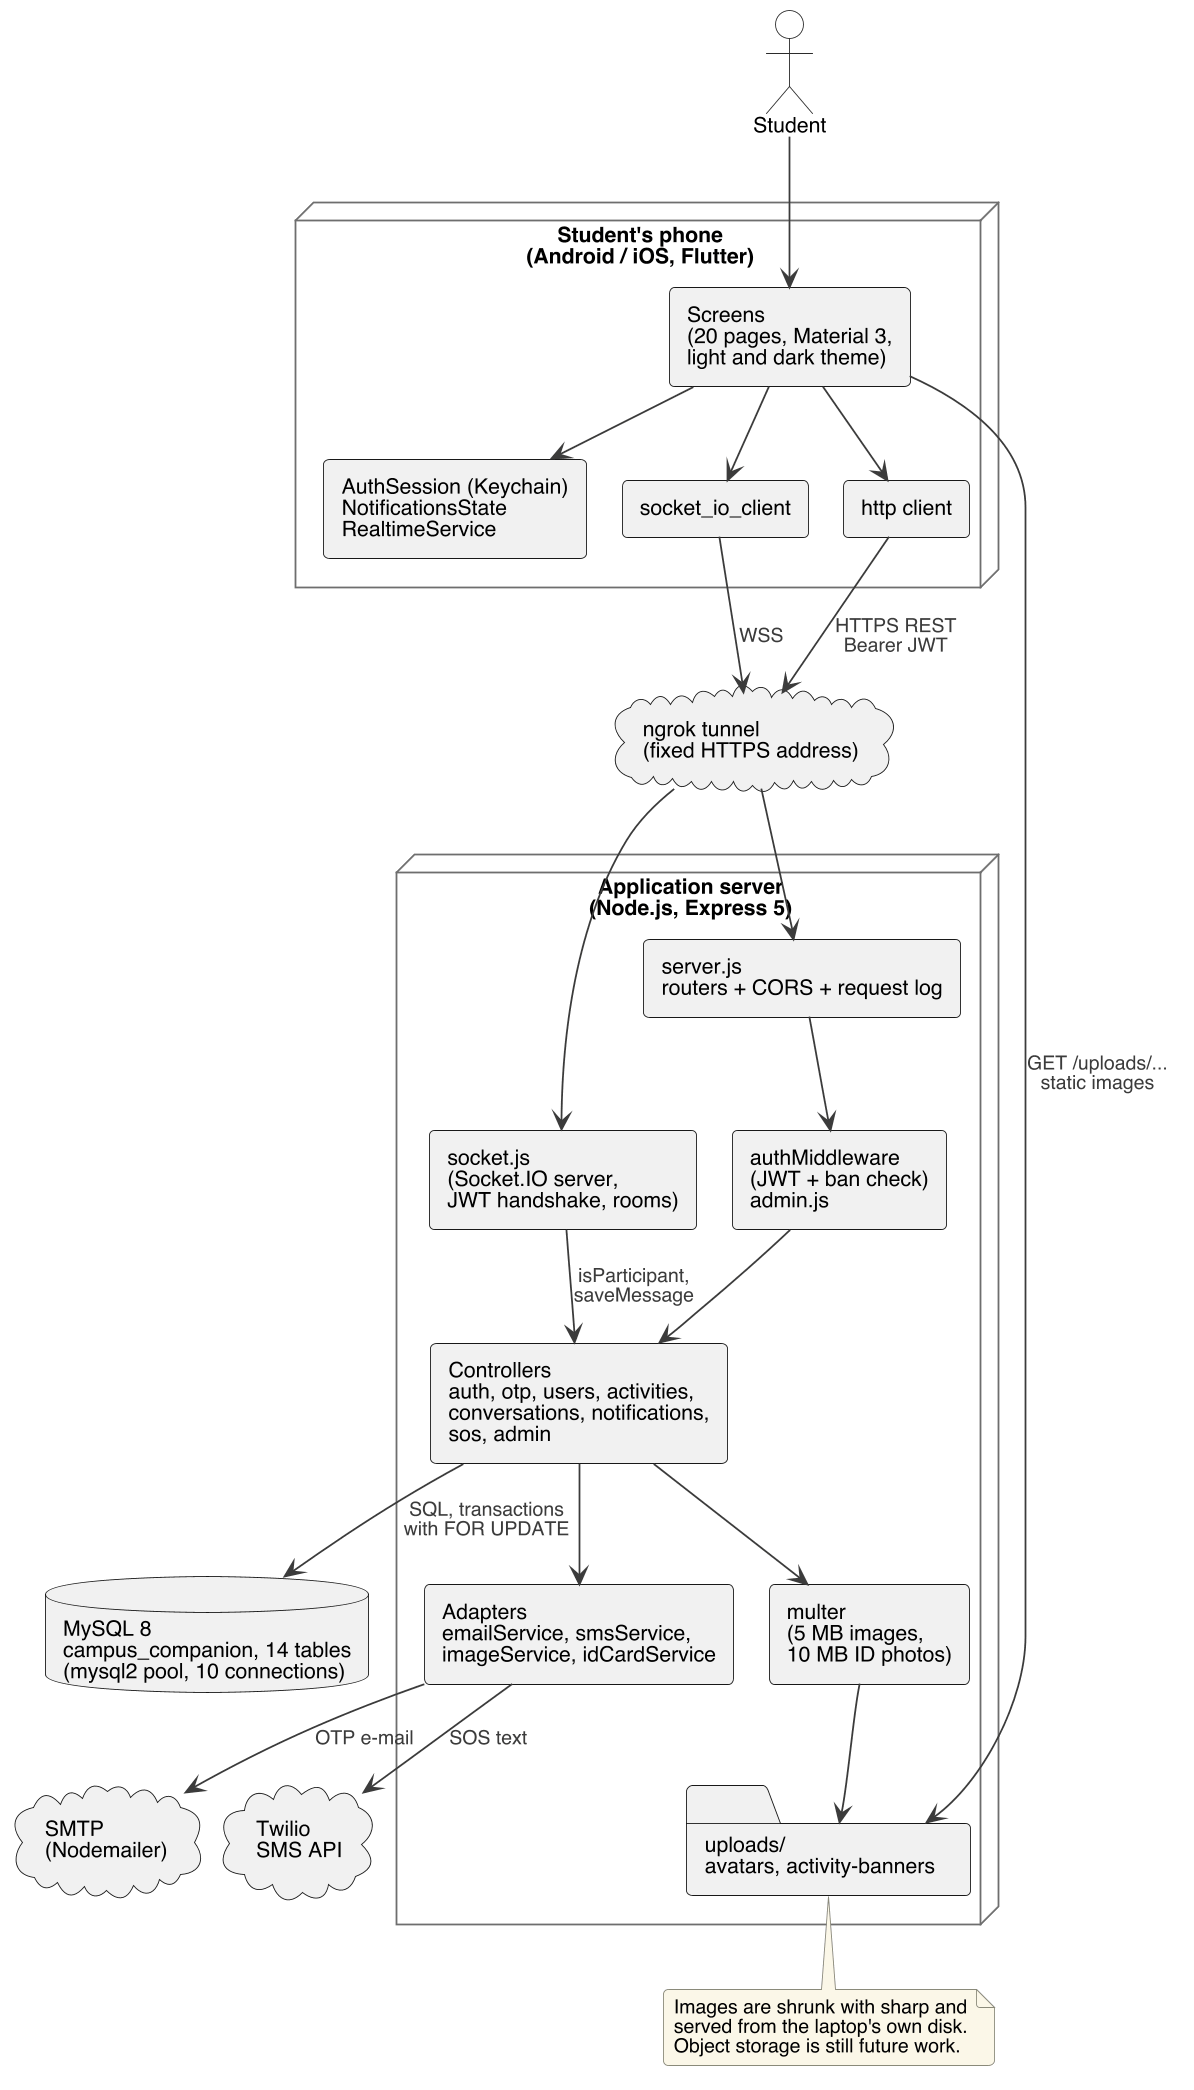
\includegraphics[width=0.62\textwidth]{figures/architecture.png}
\caption{High-level architecture of Campus Companion at the final evaluation}
\label{fig:architecture}
\end{figure}

\begin{itemize}
  \item \textbf{Presentation.} Twenty Flutter screens, themed with Material 3 in both
        light and dark, around a five-item bottom bar (Home, Discover, Host, Messages,
        Profile). Host opens a sheet asking whether the student is hosting an activity
        or an event, rather than being a screen of its own.

  \item \textbf{Application.} Seven Express routers over eight controllers, a JWT
        middleware that also refuses banned accounts, an admin guard on the moderation
        routes, and a Socket.IO server sharing the same HTTP server and signing secret.
        \texttt{migrate.js} brings an older database up to date on every start.

  \item \textbf{Adapters.} Four side-effect modules, for e-mail, SMS, image processing
        and ID card reading, isolated so that the controller logic around them can be
        read and tested without reaching the network.

  \item \textbf{Data.} MySQL 8 through a \texttt{mysql2} pool capped at ten connections,
        plus a local \texttt{uploads/} directory served as static files for avatars and
        activity banners.
  \item \textbf{Reaching it.} The server runs on a team laptop. Campus wifi isolates
        devices from one another, so phones reach it through an ngrok tunnel on a fixed
        HTTPS address, started together with the server by
        \texttt{scripts/start-demo.sh}.
\end{itemize}

\subsection{How a Request Travels}

A typical authenticated request runs as follows. The Flutter screen attaches
\texttt{Authorization: Bearer <token>} from \texttt{AuthSession} and calls the
endpoint. Express parses JSON, logs the method and path, and hands the request to the
router. The router's \texttt{verifyToken} middleware validates the signature and
expiry and writes \texttt{req.userId} onto the request, so every handler behind it can
assume an authenticated caller without repeating the check. The controller validates
its inputs, opens a transaction if it needs one, runs its queries through the pool,
and serialises the result into the \texttt{snake\_case} to \texttt{camelCase} shape the
client expects.

Real-time messages take a different path. The client opens a WebSocket and passes the
same token in the Socket.IO handshake. The server verifies it once at connection time,
then admits the socket to a room named after the conversation only after confirming
membership in \texttt{conversation\_\allowbreak participants}. A sent message is persisted first and
broadcast second, so what every participant receives is exactly what was written.

\subsection{Technology Stack}

\begin{itemize}[nosep]
  \item \raggedright\textbf{Client:} Flutter with Dart and Material 3~\cite{flutter2026}. Packages:
        \texttt{google\_fonts}, \texttt{http}, \texttt{image\_picker},
        \texttt{socket\_io\_client}, \texttt{flutter\_secure\_storage},
        \texttt{cached\_network\_image}.
  \item \textbf{Server:} Node.js with Express 5~\cite{express2026}, CommonJS modules.
  \item \textbf{Database:} MySQL 8 accessed through \texttt{mysql2/promise} with a
        connection pool~\cite{mysql2026}.
  \item \textbf{Authentication:} \texttt{bcrypt} for password hashing~\cite{provos1999}
        and \texttt{jsonwebtoken} for seven-day bearer tokens~\cite{rfc7519}.
  \item \textbf{Real time:} Socket.IO 4 over the same HTTP server~\cite{socketio2026}.
  \item \textbf{Outbound:} Nodemailer over SMTP~\cite{nodemailer2026} and the Twilio
        REST API~\cite{twilio2026}.
  \item \textbf{Uploads and images:} \texttt{multer} for multipart handling,
        \texttt{heic-convert} for HEIC and HEIF, and \texttt{sharp} for resizing and
        WebP encoding.
  \item \textbf{ID card reading:} \texttt{tesseract.js} for text and \texttt{zxing-wasm}
        for the Code~128 barcode, both running inside the server process.
  \item \textbf{Testing:} Node's built-in test runner for the API and
        \texttt{flutter\_test} for the app.
  \item \textbf{Modelling:} PlantUML for the diagrams in Chapter~\ref{ch:uml}, with the
        sources kept beside this report so the figures can be regenerated when the code
        changes~\cite{plantuml2026}.
\end{itemize}

\noindent At the final evaluation the implementation stands at roughly 3{,}150 lines of
JavaScript and 9{,}900 lines of Dart, exposing 44 REST endpoints and four Socket.IO
events, with about 1{,}000 lines of automated tests. At mid-semester the figures were
1{,}700, 6{,}400, 30 and three.

\subsection{Data Model}

Table~\ref{tab:schema} summarises the fourteen tables; three were added after mid-semester for events. Two modelling decisions are worth
calling out. First, \texttt{conversations} carries a nullable \texttt{activity\_id}:
a null value marks a direct message and a non-null value marks an activity group chat,
so one table and one message pipeline serve both. Second, join requests and
participation are separate tables rather than one table with a status column, because
a request is a transient negotiation that can be withdrawn or refused whereas
participation is a fact about who was there, and ratings hang off the latter.

\begin{table}[htbp]
\centering
\begin{tabular}{|L{4.9cm}|L{6.6cm}|}
\hline
\textbf{Table} & \textbf{Purpose and notable columns} \\
\hline
\texttt{users} & One row per student. Unique \texttt{email}, \texttt{password\_hash},
\texttt{is\_verified}, \texttt{gender}, \texttt{bio}, \texttt{avatar\_url}, the two
emergency-contact columns, the ID check status with a unique keyed hash of the roll
number, and \texttt{is\_banned} with a reason \\
\hline
\texttt{otp\_verifications} & Live one-time codes, keyed on e-mail rather than user id
so a reset code can be issued before a session exists. \texttt{purpose} separates
verification codes from reset codes \\
\hline
\texttt{activities} & Title, category, description, landmark, \texttt{starts\_at},
optional \texttt{duration\_minutes}, \texttt{max\_people}, \texttt{banner\_url},
\texttt{is\_team\_event} (marks an event) and \texttt{is\_featured} \\
\hline
\texttt{activity\_join\_requests} & One pending, accepted or declined request per
(activity, user), with \texttt{responded\_at} \\
\hline
\texttt{activity\_participants} & Confirmed membership, unique per (activity, user) \\
\hline
\texttt{conversations} & Group chat when \texttt{activity\_id} is set, direct message
when it is null \\
\hline
\texttt{conversation\_\allowbreak participants} & Membership, and the gate the socket layer checks \\
\hline
\texttt{messages} & Body, sender and timestamp; read back newest-first with a
keyset cursor \\
\hline
\texttt{ratings} & \texttt{DECIMAL(2,1)} score, optional review text and tags, unique per
(activity, rater, rated) \\
\hline
\texttt{notifications} & Five types, with a nullable \texttt{read\_at} carrying the
unread state \\
\hline
\texttt{sos\_alerts} & One coordinate pair, the contact number notified, and the
activity the student was in at the time \\
\hline
\texttt{activity\_teams} & An activity inside an event: name, spots, optional time and
optional players per team \\
\hline
\texttt{activity\_team\_members} & Who signed up for which event activity, and which
team they play in \\
\hline
\texttt{activity\_squads} & Named teams inside a team activity \\
\hline
\end{tabular}
\caption{Relational schema at the final evaluation}
\label{tab:schema}
\end{table}

\section{Implementation Details}
\label{sec:impl}

\subsection{Module 1: Identity and Account Recovery}

Registration refuses any address not ending in \texttt{@thapar.edu}, hashes the
password with bcrypt at ten salt rounds and writes the row with
\texttt{is\_verified = FALSE}. A six-digit code is generated with
\texttt{crypto.randomInt}, every earlier code for that address and purpose is deleted
so only one is ever live, and the new code is stored with a ten-minute expiry and
mailed out.

Two cases in this module needed care. An address that already exists but was never
verified is not an error: the row is reused and a fresh code is sent, so a student who
closed the app mid-sign-up can simply start again. And a login against an unverified
account does not merely fail; it sends a new code and answers 403 with a
\texttt{requiresVerification} flag, which the application uses to drop the student
straight onto the code screen.

Password recovery runs on the same machinery with \texttt{purpose = reset\_password},
which is what prevents a code issued for one flow from satisfying the other. The
request endpoint returns the same message whether or not the address has an account,
so it cannot be used to enumerate students, and the reset itself re-hashes the new
password and deletes every outstanding reset code for that address.

\subsection{Module 2: Hosting an Activity}

The host form collects a title, a category, an optional description, a date and time,
an optional duration, a capacity, and a landmark. At mid-semester four categories were
offered (Hiking, Coffee, Gaming and Sports). After feedback they became Hangout, Coffee,
Movie, Gym and Walk, plus Event, which only the event form uses; \texttt{migrate.js}
moves activities filed under the old names on start-up. Both this form and the Discover
filter read the categories from one shared list, so neither screen
can offer a value the other does not understand. The server rejects a category outside
that set, because the column is a plain \texttt{VARCHAR} with no constraint of its own.
Submitting the form runs a single transaction that inserts the
activity, enrols the host as its first participant, creates the conversation and puts
the host into it. If any of the four statements fails the whole thing rolls back, so
there is no such thing as an activity without a chat or a chat without its host.

A banner photo is a separate, optional upload afterwards, and this ordering is
deliberate. The activity already exists by the time the image is sent, so a failed
upload does not cost the host the form; the application says the activity was created
but the photo did not upload, and the host can retry.

\subsection{Module 3: Discovery and the Join Handshake}

Discovery is a single query that returns each listing together with its head count, the
host's average rating, and three flags computed for the calling student: whether they
have already joined, whether they have a request pending, and whether they were
previously declined. Putting those flags in the list response is what lets the client
render the correct button on every card without a second round trip. Filtering by
category happens on the client over the already-fetched list. The endpoint also accepts
a \texttt{search} parameter, matched as a \texttt{LIKE} clause on the title, but the
client still does not send one: the activity search box on Discover is drawn as text and
does nothing when tapped. The person icon at its right end does work, and opens a search
for people by name (Module~10). Admin-featured activities are sorted to the top.

Requesting to join is guarded by four checks, in order: the host cannot request to join
their own activity, an existing participant cannot request again, a full activity
returns 409, and an activity where the host has already declined this student returns
403. That last rule is the one product decision embedded in this module. A decline is
final for that activity, so a student cannot wear a host down by asking repeatedly.

The host's side of the handshake is the most carefully written path in the codebase. It
opens a transaction, takes \texttt{FOR UPDATE} locks on the activity and the request,
confirms the caller is the host and the request is still pending, re-checks capacity
inside the lock, inserts the participant and the conversation membership together, and
only then updates the request status. The requester is notified either way.

\subsection{Module 4: Real-Time Messaging}

Every activity has a conversation from birth, and acceptance into the activity and
admission to the chat are the same database write, so the two can never disagree.
Direct conversations are created on demand between two students and reuse an existing
one if the pair already has it.

The socket layer authenticates once at handshake time from the JWT and then checks
\texttt{conversation\_\allowbreak participants} on every room join and every send, because
membership can be revoked between connection and message. Messages are written to the
database before they are broadcast. History is fetched over REST with a
\texttt{before} cursor and a limit capped at one hundred, and reversed on the server so
the client always receives chronological order.

\subsection{Module 5: Reputation}

A rating is a half-star value from 1.0 to 5.0 stored as \texttt{DECIMAL(2,1)}. Three
conditions are enforced before one is accepted: the activity must be over, which is
computed as \texttt{starts\_at} plus \texttt{duration\_minutes}; both the rater and the
person being rated must appear in \texttt{activity\_participants} for that activity; and
nobody may rate themselves. The insert is an upsert keyed on (activity, rater, rated),
so a student can revise a score but cannot inflate anyone by rating them twice for the
same outing.

The average is computed at read time as a correlated subquery on every listing and
participant row, which is simple and correct. It is not free, and Section~\ref{sec:scalability}
notes where it would stop being appropriate.

\subsection{Module 6: Notifications}

Five events produce a notification: a new join request, an accepted request, a declined
request, a cancelled activity and a received rating. Writing one is deliberately
best-effort: \texttt{createNotification} swallows its own failure and logs it, because
a notification that fails to write must not roll back the join it was reporting.

Unread state is a nullable \texttt{read\_at} rather than a boolean, which means the
system records when something was read rather than merely that it was. The badge count
is held in a \texttt{ValueNotifier} shared across screens and refreshed on login and
whenever the notifications screen changes anything, which avoids pulling a
state-management dependency into the project for one integer.

\subsection{Module 7: Safety}

The emergency contact lives on the user row and has its own screen, moved out of the
general profile editor so that it reads as a safety feature rather than another
optional field. The server refuses an SOS outright if no contact number is on file, and
says so, rather than failing silently at the moment it matters.

When an SOS fires, the server finds the activity the student is currently in by looking
for one they have joined whose start time falls between one hour ago and three hours
ahead, collects the names of the other participants, composes a message containing a
Google Maps link and that list of companions, sends it through Twilio, and records the
alert. The value of naming the companions is that the contact receiving the text learns
not only where the student is but who they are with.

This is the one objective that is not finished. The server path above is complete and
tested (TC24), and the emergency-contact screen is in the application, but the SOS
control in the top bar still shows a ``coming soon'' message
(Figure~\ref{fig:scr-safety}d). Connecting it to the device's location service needs a
permission prompt and a confirmation step so it cannot be pressed by accident, and that
work was not done.

\subsection{Cross-Cutting: Uploads and Images}

Avatars and activity banners share one pipeline. \texttt{multer} caps the upload at
5~MB and restricts it to JPEG, PNG, WEBP, HEIC and HEIF, and its errors are wrapped so
a rejected file returns JSON rather than Express's default HTML error page. HEIC and
HEIF files are then converted to JPEG and the original is deleted, because iOS and
macOS produce HEIC by default and most browsers and Android devices cannot decode it.
Only the host may set an activity's banner, checked against the JWT rather than against
anything in the request.

Since mid-semester every upload is also shrunk before it is stored. Avatars are cropped
to 400 by 400 pixels and banners capped at 1{,}200 pixels, the phone's rotation flag is
applied, and the result is saved as WebP. A real phone photo used as an avatar went from
423~KB to 39~KB. Uploaded files are served with a thirty-day cache header and the app
keeps them in an on-device cache, which matters because the tunnel has a monthly data
allowance and many students are on mobile data.

\subsection{Module 8: Checking a Student's ID Card}
\label{sec:idcard}

The one-time code proves that a student can read mail sent to a Thapar address. It does
not prove that the person holding the phone is that student. The feasibility study
proposed closing that gap with face recognition, and a first version did exactly that:
the student uploaded a selfie and a photo of their card, and \texttt{face-api} compared
the two faces. On a real card the genuine owner scored 22\% similarity against their own
printed photograph. The portraits on the cards are small, faded and often several years
old, and no threshold separated the right person from a wrong one. The approach was
removed along with roughly 100~MB of TensorFlow dependencies.

The replacement (\texttt{idCardService.js}) reads what is printed on the card instead.
The student photographs the front and the back, and the server runs four checks in order,
stopping at the first one that fails:

\begin{enumerate}[nosep]
  \item The account's e-mail must be in the student format, an initial, a surname and a
        program with a batch year (\texttt{avasdev\_be24}). Staff-style addresses are told
        the check is for students only.
  \item OCR on the front must find ``THAPAR'' and ``IDENTITY'' or ``LIBRARY'', so a photo
        of something else is refused with advice on how to retake it.
  \item A name on the card must have the same first initial and surname as the e-mail,
        allowing one OCR slip. Only the owner of the e-mail can log in, so a borrowed card
        fails here.
  \item The Code~128 barcode on the back must decode to a roll number printed on the
        front, which shows both photos are of the same physical card.
\end{enumerate}

\noindent The roll number is then stored only as an HMAC under a unique index, so one card
can verify one account and the number itself is never kept. The photos are held in memory
for the length of the request and never written to disk. A failed check records the status
as \texttt{failed} and returns a specific message, and an admin can grant the tick by hand
when a genuine card will not scan. Figure~\ref{fig:seqid} shows the full exchange.

\subsection{Module 9: Events, and Teams Inside Them}

The first round of feedback after mid-semester was that a fest is not one activity. A
host can now choose between an activity and an event when they press Host. An event uses
the same form without a category picker, can run over several days, and can take up to
50{,}000 people. Inside it, only the host adds activities, each with a name, a number of
spots and an optional time that must fall within the event's dates. Attendees who have been
accepted into the event sign up for as many of these as have room, and leaving the event
signs them out of all of them.

An activity inside an event can be a team activity with a fixed number of players per
team, Football in teams of five for instance. Attendees then start a team or join one with
space; the number of teams is capped at the spots divided by the team size (rounded up), and team names
are unique within the activity. Sign-up and team joins run in transactions with row locks,
the same way the main join handshake does, so a last spot cannot be taken twice.

\subsection{Module 10: Reviews, Public Profiles and People Search}

A rating can now carry a written review of up to 500 characters and any of seven fixed
tags (Friendly, Punctual, Great host, Good communicator, Reliable, Respectful, Fun to be
around). The tags are a fixed list on purpose, so a profile can count them: ``Punctual
$\times$4'' says more than four separate sentences would.

Every student has a public profile showing how many activities they have hosted and
joined, their average with a star histogram, tag counts, recent reviews and what they are
hosting soon. E-mail, phone number and emergency contact are left out of the response
entirely rather than hidden by the app, and TC21 checks this. A search by name finds other
students whose e-mail is confirmed, and a profile can be reached from any host name or participant row.

\subsection{Module 11: Live Notifications}

At mid-semester a notification appeared only when the notifications screen was reloaded.
Every socket connection now also joins a personal room, \texttt{user:<id>}, and
\texttt{createNotification} pushes \texttt{notification:new} into it as soon as the row is
written. The app shows it as a banner that slides in at the top, one at a time if several
arrive together. A host sees a join request the moment it is made.

Getting this working uncovered a defect worth recording. \texttt{socket\_io\_client} reuses
one connection per server address, so the chat screen was handed the already-connected
notification socket. Its connect handler never fired, it never joined the chat room, and
new messages only appeared after leaving and reopening the chat. Closing the chat then shut
the shared socket and stopped notifications too. Chat and notifications now open separate
connections.

\subsection{Module 12: Moderation}

The study asked for reporting and moderation. Moderation is now in place. Admins are listed
in the server's \texttt{.env} file and nowhere else, so nobody can make themselves an admin
from the app, and every admin route checks this again on the server. An admin can:

\begin{itemize}[nosep]
  \item ban or unban a student with a reason. The ban is checked on every request and at
        the socket handshake, so it applies at once to tokens issued before it (TC26);
  \item delete any activity or event, and remove any review, with the people affected told
        that the Companion team removed it;
  \item give or remove the verified tick;
  \item feature an activity or event, which pins it to the top of Discover.
\end{itemize}

\noindent Admins cannot ban themselves or each other. What is still missing is the other half
of the study's proposal: an ordinary student has no way to report or block someone.

\subsection{Module 13: Staying Logged In}

The token used to live only in memory, so closing the app meant logging in again. It is now
saved in the phone's secure storage (the iOS Keychain or Android's encrypted storage) and
cleared on Log Out. On launch a start-up screen restores it and checks it against
\texttt{/api/users/me}: an expired or banned login goes back to the login page, while an
unreachable server keeps the student logged in so the app recovers once the server is back.
A related fix: logging in used to push the home screen on top of the login form, so the iOS
back swipe slid back to the filled-in login page. Login now replaces the whole navigation
stack, and a widget test checks that nothing is left to go back to.

\subsection{Module 14: Running It Outside the Lab}

Putting the app on other students' phones turned up three problems that never appear on a
simulator. Android release builds had no internet permission, because Flutter only adds it
to debug builds, and Android also blocks plain HTTP by default. Thapar's wifi isolates
devices from each other, so a phone cannot reach the laptop's address even on the same
network. And the laptop's address changes whenever the wifi does.

The answer was to stop depending on the network at all. \texttt{scripts/start-demo.sh}
starts the server and an ngrok tunnel on a fixed public HTTPS address, keeps the laptop
awake, and restarts either process if it stops. The app is built with that address passed
in as \texttt{API\_URL}. An earlier version let the server address be changed from inside
the app by long-pressing the logo; that was removed, because anyone holding the phone could
have pointed it at a server of their own and collected the next login.


% ===== CHAPTER 4: EVALUATION AND CURRENT STATUS =====

\chapter{Evaluation and Current Status}

\section{Evaluation Criteria}

\subsection{Primary Metric}

\textbf{Time to a confirmed companion (TTCC):} the elapsed time between a student
tapping \emph{Request to join} and the host accepting, measured as
\texttt{responded\_at} minus \texttt{created\_at} on the \texttt{activity\_join\_requests}
row. This is the metric because it measures the thing the product actually claims to
improve, which is how long it takes to go from wanting company to having it. Both
timestamps are already written by the system, so attribution needs no additional
instrumentation. The target for the pilot is a median TTCC under two hours for requests
made more than a day before the activity starts.

\subsection{Secondary Metrics}

\begin{itemize}
  \item \textbf{Acceptance rate:} accepted requests divided by all responded requests.
        A very high rate would suggest hosts are rubber-stamping and the approval step
        is theatre; a very low one would suggest discovery is showing students the wrong
        activities.
  \item \textbf{Fill rate:} participants at start time divided by \texttt{max\_people}.
        This is the most direct measure of whether the product succeeds at its stated
        job.
  \item \textbf{Unanswered-request rate:} requests still pending when the activity
        starts. This is the failure mode the host-approval design creates, and it needs
        to be watched rather than assumed away.
  \item \textbf{Rating coverage:} finished activities with at least one rating, divided
        by all finished activities. The reputation signal is only meaningful if people
        actually leave ratings.
  \item \textbf{Repeat participation:} students who join a second activity within two
        weeks of their first.
  \item \textbf{Safety readiness:} the share of accounts with an emergency contact on
        file, which is the precondition for SOS being any use at all.
\end{itemize}

\subsection{Pilot Plan}

Recruit twenty to thirty students from one batch, so that density is achieved inside a
single cohort rather than spread thinly across the institute. Run the platform for two
weeks on a hosted deployment over HTTPS, with the SOS path complete. Compute every
metric above directly from the database. Follow with a short questionnaire on two
points the database cannot answer: whether the host-approval step felt worth its
friction, and whether students would have gone to the activity had the application not
existed.

\section{Testing Carried Out up to Mid-Semester}

\begin{itemize}
  \item \textbf{Integration testing by live walkthrough.} Every feature has been
        exercised end to end against the real MySQL database, with real e-mail delivery
        and a real Twilio number, from both an iOS device and an Android emulator. The
        paths walked include registration through to a verified login, an expired code,
        a wrong code, the resend cooldown, a full password reset, hosting with and
        without a banner, requesting and withdrawing, accepting and declining, the
        declined-then-re-requesting refusal, joining a full activity, group and direct
        messaging across two devices simultaneously, rating before and after the end
        time, and cancelling an activity that had participants and pending requests.

  \item \textbf{Concurrency testing on the one path that needs it.} Accepting two
        requests into a single remaining place was tested with two clients, and the
        second correctly receives 409 rather than overfilling the activity.

  \item \textbf{Error-path testing on uploads.} Oversize files, disallowed types and
        HEIC photographs taken on an iPhone were each uploaded to confirm the rejection
        message is JSON and the conversion produces a JPEG that renders on Android.

  \item \textbf{Automated testing: one widget test, and that was the gap.} At
        mid-semester the Flutter project contained a single test asserting the
        application boots to the login screen, and there was no server-side suite.
        Chapter~\ref{ch:testing} describes how this was closed: 29 end-to-end server
        tests and 19 Flutter tests, all passing at the final evaluation.

  \item \textbf{Static checks.} The Flutter analyser runs clean under
        \texttt{flutter\_lints}.
\end{itemize}

\section{Status Against Objectives}

Table~\ref{tab:status} compares the mid-semester position with the final one. The pilot
was not run, so its two rows have no figures.

\begin{table}[htbp]
\centering
\begin{tabular}{|L{5.6cm}|L{2.6cm}|L{3.3cm}|}
\hline
\textbf{Item} & \textbf{Mid-semester} & \textbf{Final} \\
\hline
Objective 1: verified institutional identity & Complete & Complete, plus ID card check \\
\hline
Objective 2: hosting and join handshake & Complete & Complete, plus events and teams \\
\hline
Objective 3: per-activity group chat & Complete & Complete \\
\hline
Objective 4: post-activity ratings & Complete & Complete, plus reviews and tags \\
\hline
Objective 5: SOS to an emergency contact & Server done, button pending & Unchanged: button still pending \\
\hline
Objective 6: measurable outcomes & Instrumented & Instrumented; pilot not run \\
\hline
Database tables & 11 & 14 \\
\hline
REST endpoints & 30 & 44 \\
\hline
Socket.IO events & 3 & 4 \\
\hline
Client screens & 16 & 20 \\
\hline
Server source (JavaScript) & $\approx$ 1{,}700 lines & $\approx$ 3{,}150 lines \\
\hline
Client source (Dart) & $\approx$ 6{,}400 lines & $\approx$ 9{,}900 lines \\
\hline
Automated tests & 2 & 48 (all passing) \\
\hline
Upload size limit & 5 MB & 5 MB (10 MB for ID photos) \\
\hline
One-time code lifetime / resend cooldown & 10 min / 60 s & 10 min / 60 s \\
\hline
Median TTCC, fill rate (pilot) & pending & not measured \\
\hline
\end{tabular}
\caption{Status at mid-semester and at the final evaluation}
\label{tab:status}
\end{table}

\section{Progress Against the Plan}

Table~\ref{tab:schedule} maps the planned build order against what was delivered. The
second half did not follow the plan in order. Persistent sessions, a reachable
deployment and the test suite were done; the SOS wiring and the pilot were not, and
several features that were never in the plan (ID card checking, events, moderation,
reviews) took their place.

\begin{table}[htbp]
\centering
\begin{tabular}{|L{1.6cm}|L{7.4cm}|L{2.4cm}|}
\hline
\textbf{Week} & \textbf{Increment} & \textbf{Status} \\
\hline
1--2 & Schema, Express skeleton, registration with OTP verification, JWT login & Done \\
\hline
3 & Flutter shell, theming, five-tab navigation, profile and avatar upload & Done \\
\hline
4 & Hosting, discovery, category filter, join requests & Done \\
\hline
5 & Host review of requests, accept and decline under transaction, notifications & Done \\
\hline
6 & Activity conversations over Socket.IO, direct messages, post-activity ratings & Done \\
\hline
7--8 & SOS wired to device location & Not done \\
\hline
7--8 & HTTPS deployment reachable from any network & Done, via a tunnel to the laptop \\
\hline
9--10 & Automated test suite, persistent sessions & Done \\
\hline
9--10 & Pagination of Discover & Not done (measured in Ch.~\ref{ch:results}) \\
\hline
--- & ID card check, events and teams, reviews, live notifications, moderation & Done (unplanned) \\
\hline
11--12 & Pilot with one batch, metric collection & Not done \\
\hline
11--12 & Final report & Done \\
\hline
\end{tabular}
\caption{Planned increments against what was delivered}
\label{tab:schedule}
\end{table}

\section{Scalability}
\label{sec:scalability}

\begin{enumerate}
  \item \textbf{The application tier is stateless and can be replicated.} Sessions are
        JWTs rather than server memory, so a second instance behind a load balancer
        needs no shared session store. The one qualification is Socket.IO, which would
        need a Redis adapter to broadcast across instances; this is a configuration
        change rather than a redesign.

  \item \textbf{The database is the first thing that will need attention, and the
        rating average is the first query within it.} Average rating is computed as a
        correlated subquery on every row of every listing. At a few hundred activities
        this is invisible; at campus scale it should become a maintained aggregate on
        the user row, updated when a rating is written. Measuring it for the final
        report (Section~\ref{sec:scaling}) showed this prediction was too pessimistic:
        with 4{,}000 activities the whole Discover query still takes under 40~ms, and the
        size of the response is the bigger problem.

  \item \textbf{Listings are not paginated.} \texttt{GET /api/activities} returns every
        matching activity. Section~\ref{sec:scaling} measures what that costs: the
        response grows by about 0.43~KB per activity, so at 4{,}000 activities each
        Discover load sends 1.7~MB. Keyset pagination on \texttt{starts\_at} is the fix,
        and the message history endpoint already works this way.

  \item \textbf{Uploads sit on the application server's disk.} That is the one genuine
        obstacle to running more than one instance. Shrinking every upload to WebP cut
        their size by about ten times, but moving them to object storage is still
        future work.
\end{enumerate}

\section{Analysis}
\label{sec:analysis}

\noindent\textbf{Objectives met at mid-semester.} Four of the six objectives were
complete and working against the real database. The fifth was complete on the server and
unfinished in the interface. The sixth was instrumented and waiting on the pilot. The final
position is in Table~\ref{tab:status}.

\medskip
\noindent\textbf{Beyond the original mid-term plan.} Before mid-semester, three things shipped that were not
in the plan for the first half: the full password-reset flow, which was scheduled for
week nine and was pulled forward once the OTP machinery made it cheap; server-side HEIC
conversion, which was not anticipated at all until testing on an iPhone showed banners
rendering as broken images on Android; and direct conversations, which were scheduled
with the second-half messaging work.

\medskip
\noindent\textbf{Problems encountered and how they were resolved.}

\begin{itemize}
  \item Accepting two join requests into one remaining place could overfill an activity,
        because the capacity check and the insert were separate statements. Both were
        moved inside a transaction with \texttt{FOR UPDATE} locks on the activity and
        request rows.

  \item HEIC uploads from Apple devices were being rejected outright, and then, once
        accepted, rendered as broken images elsewhere. Resolved in two steps across two
        commits: converting HEIC and HEIF to JPEG on the server, and then fixing the
        content type the client was attaching to the multipart request, which was the
        reason the files were rejected in the first place.

  \item Deleting an activity left orphaned messages, conversation memberships and
        notifications behind. The delete now runs as one transaction across eight tables,
        nulling the activity reference on rows worth keeping and removing the rest.

  \item A declined student could re-request indefinitely, since the upsert simply reset
        the row to pending. A declined request is now terminal for that activity.

  \item The emergency contact was buried inside the general profile editor, where it read
        as one more optional field. It was moved to its own screen with an explanation of
        exactly when the number would be used.
\end{itemize}

\medskip
\noindent\textbf{Known weaknesses at mid-semester, and what happened to them.} Five were
recorded. There was no server-side test suite; there now is one (Chapter~\ref{ch:testing}).
The session token lived in memory only; it is now kept in secure storage (Module~13). The
API ran over plain HTTP and was not deployed; phones now reach it over HTTPS through a
tunnel, although the server is still a laptop (Module~14). A rating was shown without its
count; the profile now shows the count and a star histogram, but activity cards on Discover
still show the average alone. And the activity search field on Discover is still drawn but
not connected.

One further defect was found while this report was being written rather than during
testing, and how it was found is worth recording. The host form offered a
``More\ldots'' chip beside the four real categories, and selecting it posted
``More\ldots'' as the activity's category. Discover filtered against the four real
ones, so an activity filed that way was reachable only under ``All Activities''. Every
manual walkthrough had picked a real category, so nothing ever exercised it; it surfaced
only when the two screens were read side by side to check a sentence in
Section~\ref{sec:impl}. It has since been fixed. Both screens now read one shared list,
Discover's chip row is built from that same list, the API refuses a category outside it,
and a unit test asserts that every category the host form can post has a chip to find it
under. That test is the second in the project, and the exercise is a fair argument for
the suite scheduled in week nine: the defect was cheap to fix and would have been cheaper
still to catch.


% ===== CHAPTER 5: TESTING =====

\chapter{Testing}
\label{ch:testing}

At mid-semester the project had one widget test, and Section~\ref{sec:analysis} called
that the biggest hole in the work. This chapter records how it was closed. Testing ran at
four levels: unit and widget tests inside the Flutter app, end-to-end tests that drive the
real server and database through its public API, system testing of the finished app on an
iPhone simulator, and static analysis.

\section{Test Plan and Environment}

\begin{table}[H]
\centering
\begin{tabular}{|L{3.2cm}|L{8.3cm}|}
\hline
\textbf{Level} & \textbf{What it covers and how it runs} \\
\hline
Unit and widget (app) & 19 tests in \texttt{frontend/test}, run with
\texttt{flutter test}. They check the host form's inputs, the activity/event chooser,
the category list, the notification banner, date formatting, the saved login and the
navigation stack after login. \\
\hline
End-to-end (server) & 29 tests in \texttt{backend/test/api.test.js}, run with
\texttt{npm test} using Node's built-in test runner. Each test signs up its own users
through the real API, so every check passes through routing, the JWT middleware, the
controllers, MySQL transactions and, for TC23, the Socket.IO server. \\
\hline
System (manual) & The app built for an iPhone 17 Pro simulator and pointed at the test
server, walked through every user-facing case with fictional seeded students.
Screenshots are in Section~\ref{sec:screens}. \\
\hline
Static analysis & \texttt{flutter analyze} with the \texttt{flutter\_lints} rules. \\
\hline
\end{tabular}
\caption{Levels of testing}
\label{tab:testlevels}
\end{table}

\noindent\textbf{Environment.} A MacBook Air (Apple M3, 8~GB) running macOS~27, Node.js
24.4, MySQL 9.7 and Flutter 3.47, with the iOS 26.5 simulator.

\medskip
\noindent\textbf{Keeping test data away from real data.} The server tests create accounts,
send one-time codes and ban users, so they never touch the development database. They run
against a separate database, \texttt{campus\_companion\_test}, built from
\texttt{schema.sql}, and the suite refuses to start unless the database name contains
``test''. The server under test sends mail to a small SMTP sink on the same machine that
accepts and discards everything, and is given dummy Twilio credentials, so no e-mail or text
message reaches a real person. Codes are read from the \texttt{otp\_verifications} table
instead of an inbox. The suite was run three times in a row against the same database
without a failure, so it does not depend on starting from an empty one.

\section{Server Test Cases}

Table~\ref{tab:apitests} lists every server test case with the result of the final run on
20 November 2026. ``Expected'' is what the test asserts, not a paraphrase of it.

\begin{longtable}{|p{1.0cm}|L{4.2cm}|L{4.4cm}|p{1.4cm}|}
\caption{End-to-end server test cases and results}\label{tab:apitests}\\
\hline
\textbf{ID} & \textbf{Scenario} & \textbf{Expected} & \textbf{Result} \\
\hline
\endfirsthead
\hline
\textbf{ID} & \textbf{Scenario} & \textbf{Expected} & \textbf{Result} \\
\hline
\endhead
\hline
\endfoot
TC01 & Register with a \texttt{@gmail.com} address & 400, message names \texttt{@thapar.edu} & Pass \\ \hline
TC02 & Register without a gender & 400, ``Gender is required'' & Pass \\ \hline
TC03 & Log in before entering the code & 403 with \texttt{requiresVerification} & Pass \\ \hline
TC04 & Enter a wrong code, then the right one & 400 ``Incorrect'', then 200 & Pass \\ \hline
TC05 & Enter a code after it has expired & 400 ``expired'' & Pass \\ \hline
TC06 & Ask for a new code within 60 s & 429 & Pass \\ \hline
TC07 & Register an already verified address & 409 & Pass \\ \hline
TC08 & Wrong password vs.\ unknown address & Both 401 with the same message & Pass \\ \hline
TC09 & Forgot password, known vs.\ unknown address; reset with a short then a valid password & Same 200 message for both; 400 for short; old password then refused, new one accepted & Pass \\ \hline
TC10 & Use a sign-up code to reset a password & 400 & Pass \\ \hline
TC11 & Call a protected route with no token or a forged one & 401 both times & Pass \\ \hline
TC12 & Host with category ``More\ldots'' or ``Event'' & 400 both times & Pass \\ \hline
TC13 & Host an activity & Host is a participant and a member of its chat & Pass \\ \hline
TC14 & Host asks to join their own activity & 400 & Pass \\ \hline
TC15 & A third student lists or accepts requests & 403; the host's accept returns 200 & Pass \\ \hline
TC16 & Host accepts a request & Guest is added to the group chat & Pass \\ \hline
TC17 & Declined student asks again & 403 & Pass \\ \hline
TC18 & Ask to join a full activity & 409 & Pass \\ \hline
TC19 & Two accepts sent at the same instant for the last place & One 200 and one 409; exactly two participants & Pass \\ \hline
TC20 & Rate before the end; after it, rate self, rate 4.3, rate as an outsider, then a valid 4.5 with one real and one made-up tag & 400; 400; 400; 403; 200 with only the real tag stored & Pass \\ \hline
TC21 & View another student's public profile & 200, no e-mail, phone or emergency contact in the response & Pass \\ \hline
TC22 & Event with a Football activity in teams of 2; outsider signs up; accepted guest joins directly; guest starts a team & Refused; 400 (must join a team); team created & Pass \\ \hline
TC23 & Host sends a chat message; an outsider tries to join the room and send & Member receives it live; outsider refused both times & Pass \\ \hline
TC24 & SOS with no emergency contact saved & 400, message asks for a contact & Pass \\ \hline
TC25 & Ordinary user calls an admin route & 403 & Pass \\ \hline
TC26 & Admin bans a user who is already logged in & Old token 403, login 403 with the reason, socket refused; admin cannot ban self & Pass \\ \hline
TC27 & Upload a 6~MB avatar, then a text file & 400 JSON both times & Pass \\ \hline
TC28 & ID check with one photo, then with two blank photos & 400; then 422 \texttt{NOT\_THAPAR\_CARD}, status \texttt{failed} & Pass \\ \hline
TC29 & ID check from a non-student address & 422 \texttt{EMAIL\_FORMAT} & Pass \\ \hline
\end{longtable}

\noindent The one positive ID card case, a real card verifying its owner, is not in the
automated suite because it needs photographs of a real student's card, which do not belong
in a repository. It was tested by hand on 19 November against both sides of a real card:
the owner passed from two different front photos, and another student's e-mail, swapped
photos, a second front photo instead of the back, and a non-student e-mail were each refused
with their own message.

\section{App Test Cases}

\begin{table}[H]
\centering
\begin{tabular}{|L{3.3cm}|p{1.1cm}|L{5.6cm}|p{1.4cm}|}
\hline
\textbf{File} & \textbf{Tests} & \textbf{What is checked} & \textbf{Result} \\
\hline
\texttt{\footnotesize categories} & 4 & Every category the host form can post has a Discover chip; no duplicates; the ``All'' chip comes first and is not itself postable & Pass \\
\hline
\texttt{\footnotesize host\_choice} & 4 & The Host button offers activity or event; each opens the right form; the event form has no category picker; Event is never offered for an ordinary activity & Pass \\
\hline
\texttt{\footnotesize host\_inputs} & 3 & Number fields accept typed values and clamp them; two side by side at phone width still show their digits; the date and time sheet returns what was picked & Pass \\
\hline
\texttt{\footnotesize when\_format} & 3 & Single-day times, multi-day date ranges, and an event that is still running counts as not ended & Pass \\
\hline
\texttt{\footnotesize notification\_popup} & 2 & A pushed notification slides in and hides; several arrive one at a time & Pass \\
\hline
\texttt{\footnotesize auth\_session} & 1 & A login survives a restart until Log Out & Pass \\
\hline
\texttt{\footnotesize login\_stack} & 1 & After login there is nothing to swipe back to & Pass \\
\hline
\texttt{\footnotesize widget} & 1 & With no saved login the app opens on the login screen & Pass \\
\hline
\end{tabular}
\caption{Flutter unit and widget tests}
\label{tab:fluttertests}
\end{table}

\section{Test Runs}

Figures~\ref{fig:run-api} and~\ref{fig:run-flutter} are the console output of the final
runs, unedited apart from line length. \texttt{flutter analyze} reported ``No issues found''
on the same code.

\begin{figure}[H]
\centering
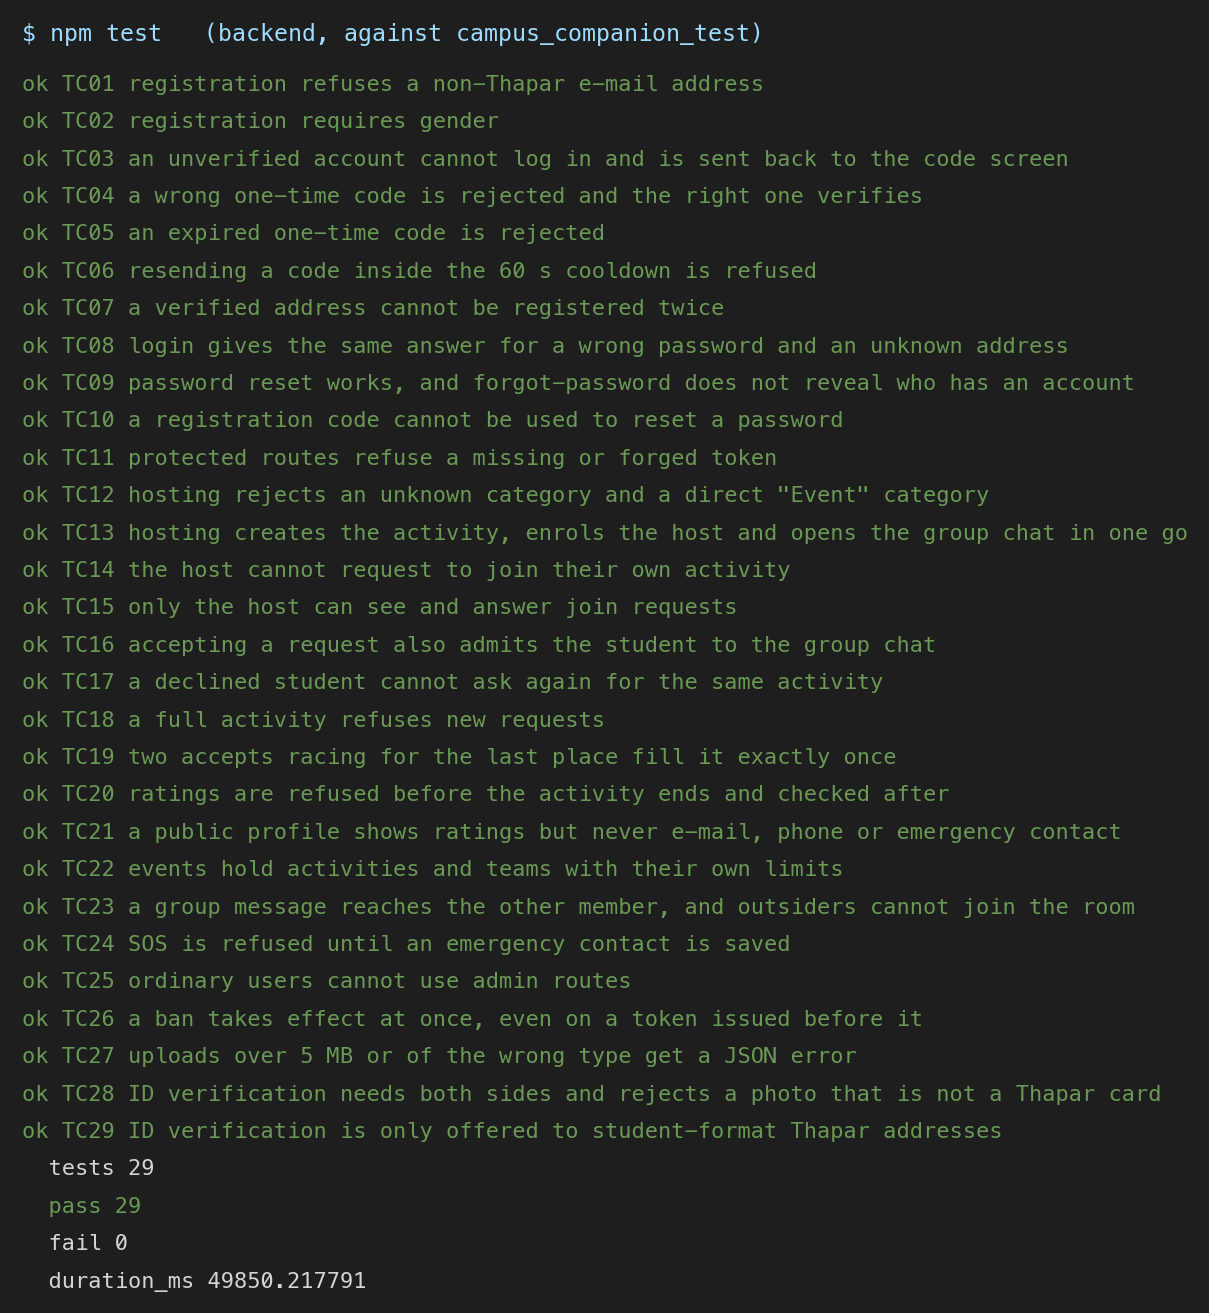
\includegraphics[width=\textwidth]{figures/charts/run-api-tests.png}
\caption{Final run of the server suite: 29 of 29 passing}
\label{fig:run-api}
\end{figure}

\begin{figure}[H]
\centering
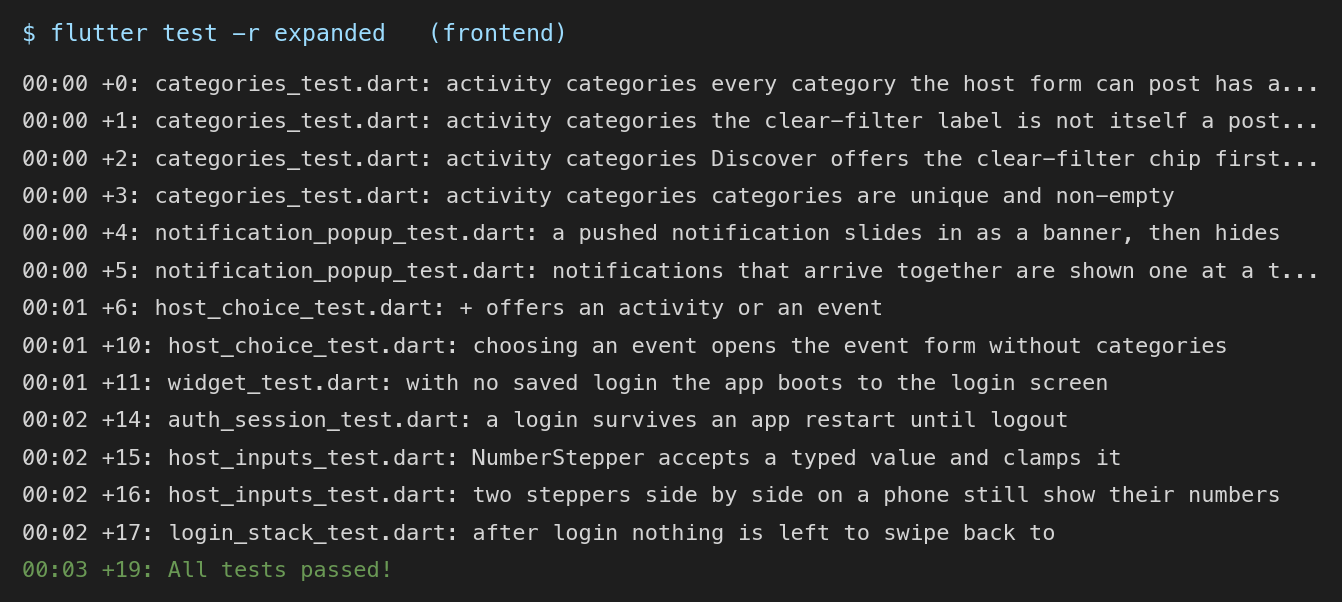
\includegraphics[width=\textwidth]{figures/charts/run-flutter-tests.png}
\caption{Final run of the Flutter suite: 19 of 19 passing}
\label{fig:run-flutter}
\end{figure}

\section{System Testing on the Simulator}
\label{sec:screens}

For system testing the app was built for the iPhone 17 Pro simulator against the test
server, and the database was filled with five fictional students, six activities, one event
with three activities inside it, a finished walk with ratings and reviews, and a short group
chat. Figures~\ref{fig:scr-join} to~\ref{fig:scr-safety} show the screens as they
appeared, each labelled with the test case it supports.

\newcommand{\screen}[2]{%
  \begin{minipage}[t]{0.29\textwidth}\centering
    \includegraphics[width=\linewidth]{figures/screens/#1}\\[2pt]
    {\footnotesize #2}
  \end{minipage}}

\begin{figure}[p]
\centering
\screen{01-login.png}{(a) Login; only \texttt{@thapar.edu} accepted (TC01, TC08)}\hfill
\screen{04-discover.png}{(b) Discover with the featured event pinned and category chips (TC12)}\hfill
\screen{14-host-choice.png}{(c) Host asks: activity or event}\\[10pt]
\screen{15-host-form.png}{(d) Host form with the five categories (TC12, TC13)}\hfill
\screen{05-activity-host.png}{(e) Host's view with two pending requests (TC15)}\hfill
\screen{06-accepted.png}{(f) After accepting Dev: 3/4 people, Dev under Who's In (TC16)}
\caption{Signing in, browsing, hosting and the join handshake}
\label{fig:scr-join}
\end{figure}

\begin{figure}[p]
\centering
\screen{07-group-chat.png}{(a) Group chat opened from the activity page (TC23)}\hfill
\screen{08-event.png}{(b) Event with Football in teams of five and the Red Hawks team (TC22)}\hfill
\screen{10-notifications.png}{(c) Notifications for acceptance, reviews and requests}\\[10pt]
\screen{09-profile.png}{(d) Own profile: 4.5 from 3 ratings, histogram and tags (TC20)}\hfill
\screen{16-public-profile.png}{(e) Another student's public profile, with no contact details (TC21)}\hfill
\screen{17-admin-profile.png}{(f) The same profile seen by an admin: Ban and Give red tick (TC25, TC26)}
\caption{Chat, events, notifications, profiles and moderation}
\label{fig:scr-profile}
\end{figure}

\begin{figure}[p]
\centering
\screen{18-verify-id.png}{(a) ID card check for an unverified account (TC28)}\hfill
\screen{11-settings.png}{(b) Settings for a verified student, with the red tick}\hfill
\screen{12-emergency-contact.png}{(c) Emergency contact saved (TC24)}\\[10pt]
\screen{13-sos.png}{(d) Pressing SOS still shows ``SOS isn't set up yet, coming soon''}
\caption{Identity and safety}
\label{fig:scr-safety}
\end{figure}

\clearpage
\section{Defects Found During Final Testing}

Writing and running the tests found the following. Defects found and fixed earlier, while
the features were being built, are recorded in the journal in Chapter~\ref{ch:journal}.

\begin{enumerate}
  \item \textbf{\texttt{schema.sql} failed on a fresh MySQL install.} It used
        \texttt{ADD COLUMN IF NOT EXISTS}, which only MariaDB supports, so creating the
        test database stopped at line 19 with only the \texttt{users} table made. Nobody
        had hit it because the development database predates those lines. Fixed: every
        table now declares all its columns, and \texttt{migrate.js} covers older databases.
  \item \textbf{TC28 passed for the wrong reason.} Its first version used a non-student
        address, so the request was refused on the e-mail format before the card photos
        were ever read. The test passed while checking nothing about the card. It was
        caught because the test took 120~ms, too fast for OCR to have run. Fixed: TC28 now
        uses a student-format address and asserts \texttt{NOT\_THAPAR\_CARD}, and the
        e-mail check got its own case, TC29.
  \item \textbf{TC26 only worked on an empty database.} On a database where the test admin
        account already existed with another password, it failed before reaching the ban.
        Fixed by giving that account the run's password first.
  \item \textbf{The activity search box on Discover does nothing} (Section~\ref{sec:impl}).
        Found while taking the screenshots. Not fixed.
  \item \textbf{The SOS control is still a placeholder} (Figure~\ref{fig:scr-safety}d). Known
        since mid-semester. Not fixed.
\end{enumerate}


% ===== CHAPTER 6: RESULTS AND ANALYSIS =====

\chapter{Results and Analysis}
\label{ch:results}

The evaluation criteria in Chapter~4 were written around a pilot with real students: time
to a confirmed companion, acceptance rate, fill rate. The pilot did not happen. The
development database holds seven accounts and seven activities created by the team, and
computing a median from five join requests would not mean anything. This chapter therefore
measures the system rather than its use: how fast it answers, how it behaves as load and
data grow, how much of it is tested, and how it grew over the semester. Every number here
was measured on 20 November 2026 on the machine described in Chapter~\ref{ch:testing}, with
the server, the database and the load generator on the same laptop. That leaves out the
network, and through the ngrok tunnel a phone will see tens of milliseconds more on every
request.

\section{Response Times}

Each endpoint was called 300 times in a row by a logged-in student after five warm-up calls
(60 times for login). Figure~\ref{fig:latency} shows the median and the 95th percentile.

\begin{figure}[htbp]
\centering
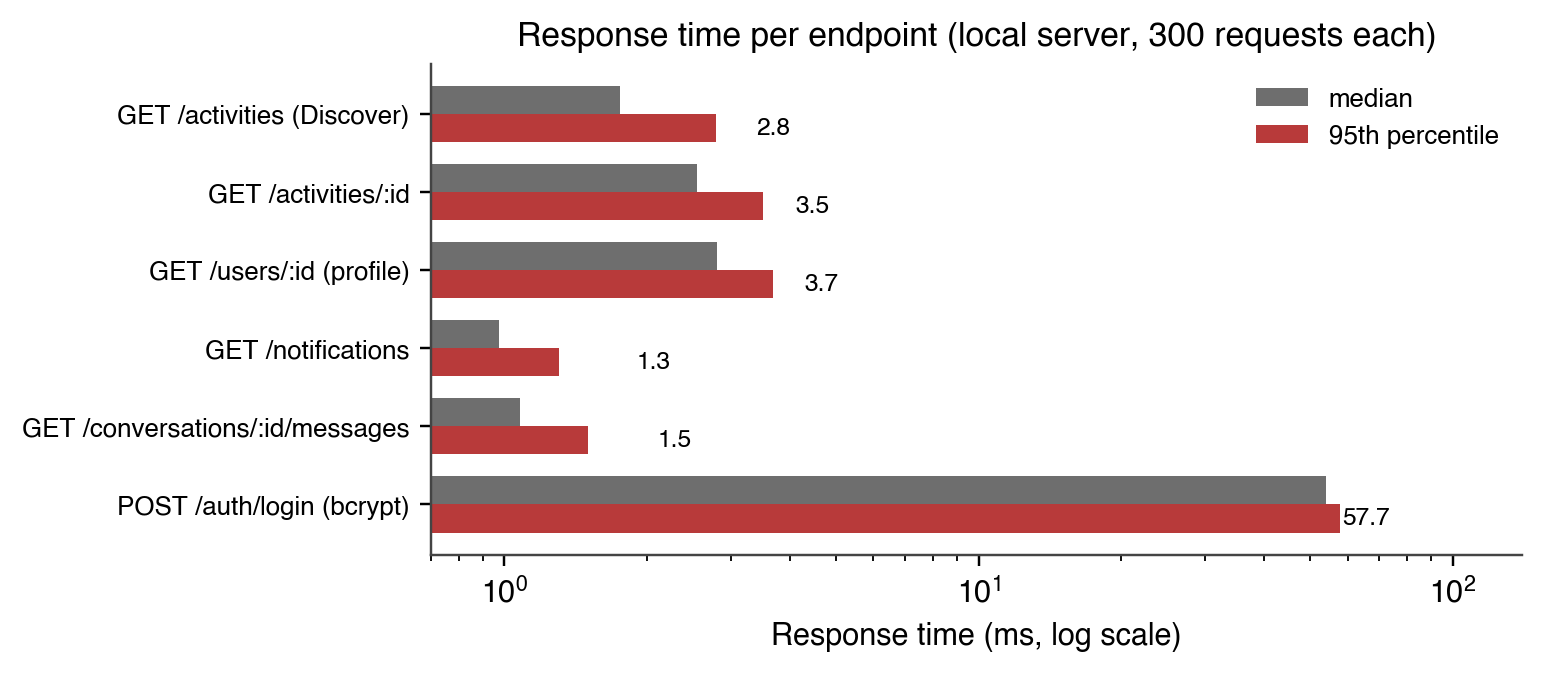
\includegraphics[width=0.92\textwidth]{figures/charts/chart-latency.png}
\caption{Server response time per endpoint}
\label{fig:latency}
\end{figure}

Every read the app makes on a normal screen answers in under 4~ms at the 95th percentile.
The profile is the slowest of them at 2.8~ms median, because it runs six queries (the user,
counts, histogram, tag counts, recent reviews and upcoming activities). Login is twenty times slower than
anything else, at 54~ms, and that is deliberate: bcrypt with ten rounds is meant to be slow,
so that a stolen password table is expensive to attack. Login happens once per device now
that sessions are saved, so its cost is paid rarely.

\section{Behaviour Under Concurrent Load}

Figure~\ref{fig:concurrency} shows Discover, the busiest screen, requested 400 times by 1, 5,
10, 25 and 50 clients at once.

\begin{figure}[htbp]
\centering
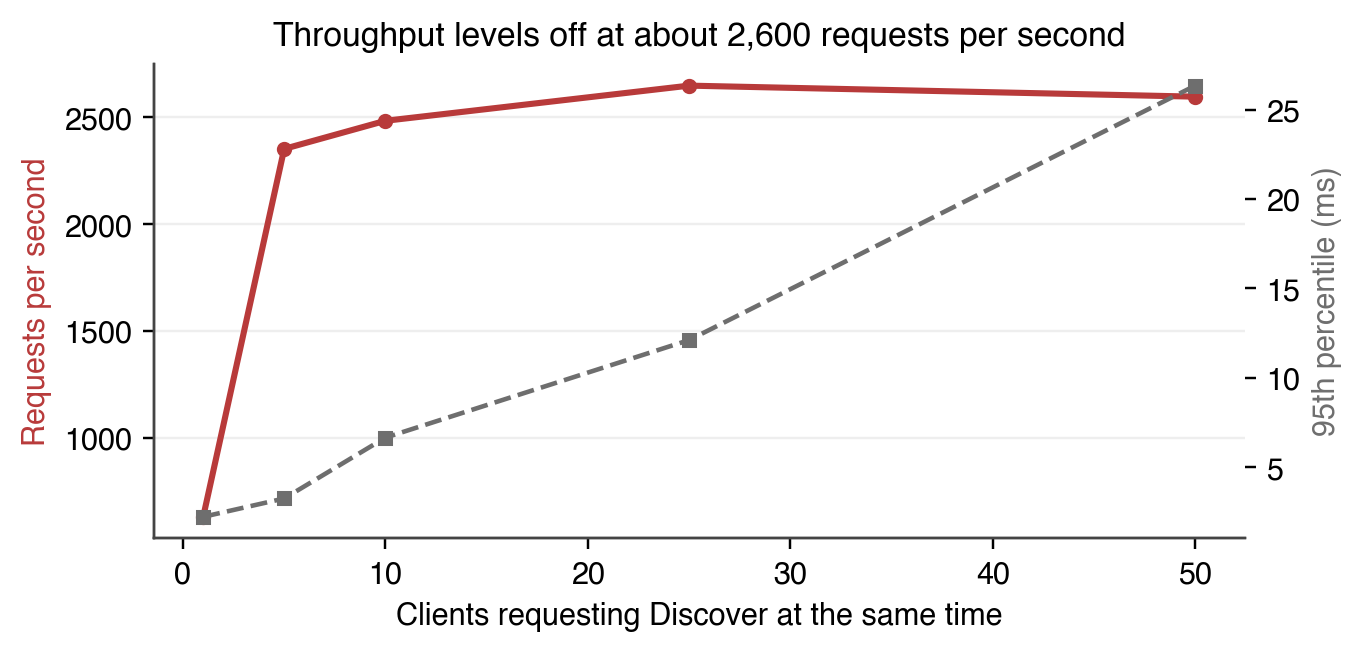
\includegraphics[width=0.92\textwidth]{figures/charts/chart-concurrency.png}
\caption{Throughput and 95th-percentile latency as concurrent clients increase}
\label{fig:concurrency}
\end{figure}

One client reaches 631 requests a second. Throughput climbs to about 2{,}350 at five clients
and then flattens at roughly 2{,}600, while the 95th percentile keeps rising, from 3.3~ms at
five clients to 26~ms at fifty. That is the shape of a single Node.js process using one core
fully: past that point extra clients only queue. For context, ten thousand
students each opening Discover once a minute would need under 170 requests a second. Capacity is not what limits this deployment; the laptop being switched off is.

\section{How Discover Scales With Data}
\label{sec:scaling}

The mid-semester report predicted that the average-rating subquery would be the first thing
to slow down. To check, activities were added to the test database in steps up to 4{,}000
and Discover was timed 30 times at each size (Figure~\ref{fig:scaling}).

\begin{figure}[htbp]
\centering
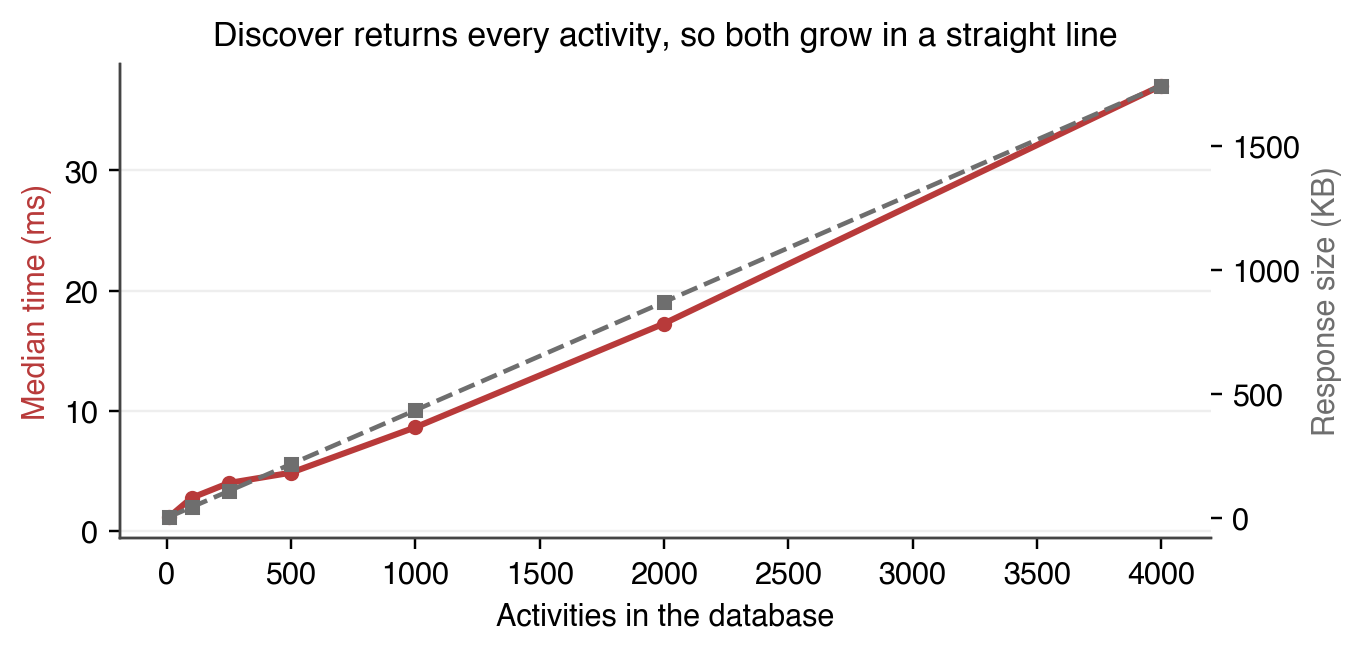
\includegraphics[width=0.92\textwidth]{figures/charts/chart-discover-scaling.png}
\caption{Discover response time and response size against the number of activities}
\label{fig:scaling}
\end{figure}

\begin{table}[htbp]
\centering
\begin{tabular}{|r|r|r|r|}
\hline
\textbf{Activities} & \textbf{Median (ms)} & \textbf{95th pct (ms)} & \textbf{Response (KB)} \\
\hline
10 & 1.2 & 2.8 & 5 \\
100 & 2.7 & 3.4 & 44 \\
500 & 4.8 & 6.1 & 217 \\
1{,}000 & 8.6 & 9.8 & 434 \\
2{,}000 & 17.3 & 19.0 & 870 \\
4{,}000 & 37.1 & 39.7 & 1{,}741 \\
\hline
\end{tabular}
\caption{Discover at increasing data sizes}
\label{tab:scaling}
\end{table}

Both lines are straight. Time grows by about 9~ms per thousand activities and the response
by about 0.43~KB per activity. The prediction was half right. The query does get slower, but
at 4{,}000 activities it still finishes in under 40~ms, which no student would notice. The
response size is the real problem: 1.7~MB sent on every visit to Discover, over mobile data,
through a tunnel with a monthly allowance. Pagination on \texttt{starts\_at}, sending the
next twenty activities as the student scrolls, would hold the response at about 9~KB
whatever the table size. That is the most useful single change left on the server.

\section{Test Coverage}

\begin{figure}[htbp]
\centering
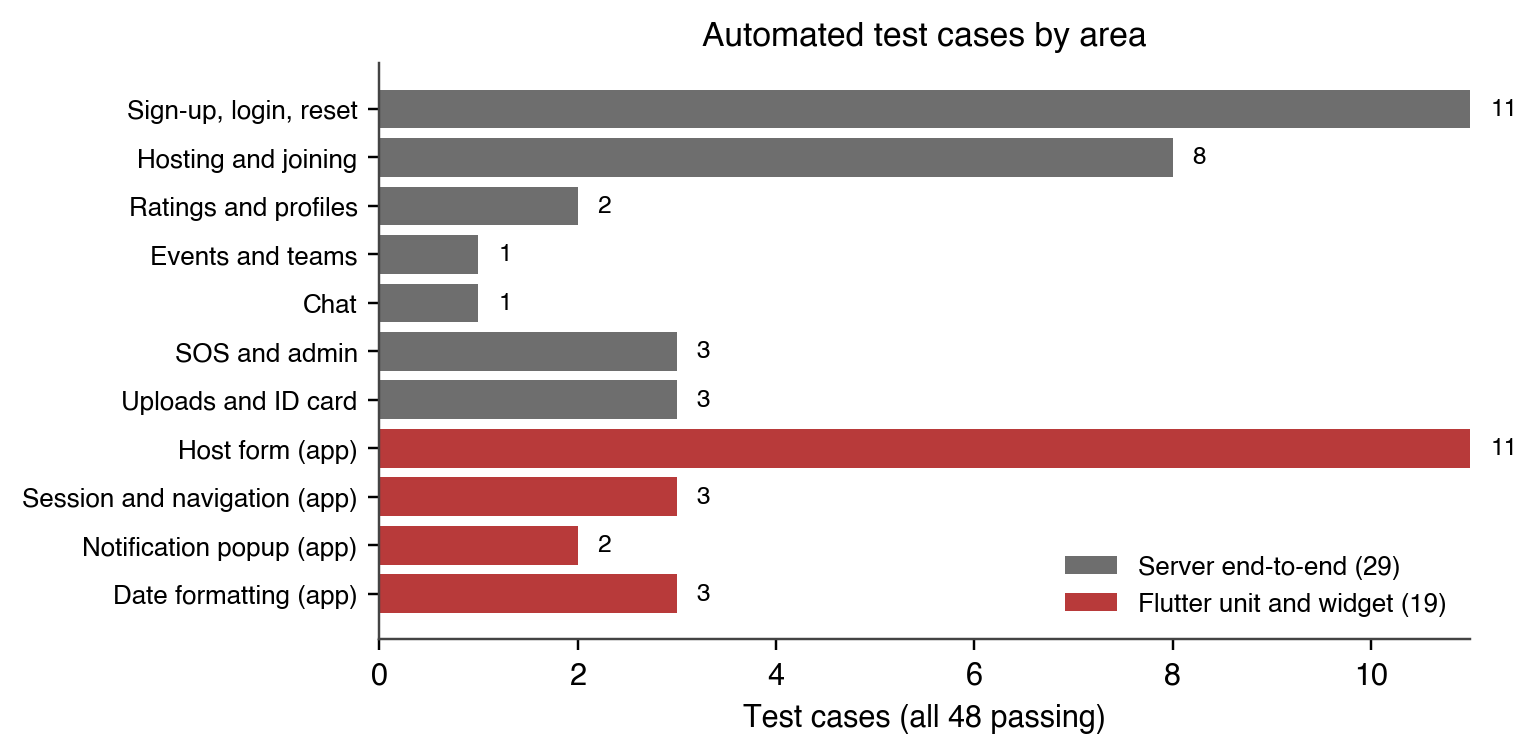
\includegraphics[width=0.92\textwidth]{figures/charts/chart-tests.png}
\caption{The 48 automated test cases by area}
\label{fig:testareas}
\end{figure}

Figure~\ref{fig:testareas} shows where the 48 tests sit. The server suite is weighted toward
sign-up and the join handshake, the two places where a mistake would let the wrong person in.
Chat, events and ratings have fewer cases each. The app tests concentrate on the host form,
which has the most input handling. What no automated test covers is the look and flow of the
screens themselves; Section~\ref{sec:screens} covered those by hand. The SOS endpoint is
tested only for refusing a student without a contact, because a passing test would send a
real text message.

\section{How the Project Grew}

\begin{figure}[htbp]
\centering
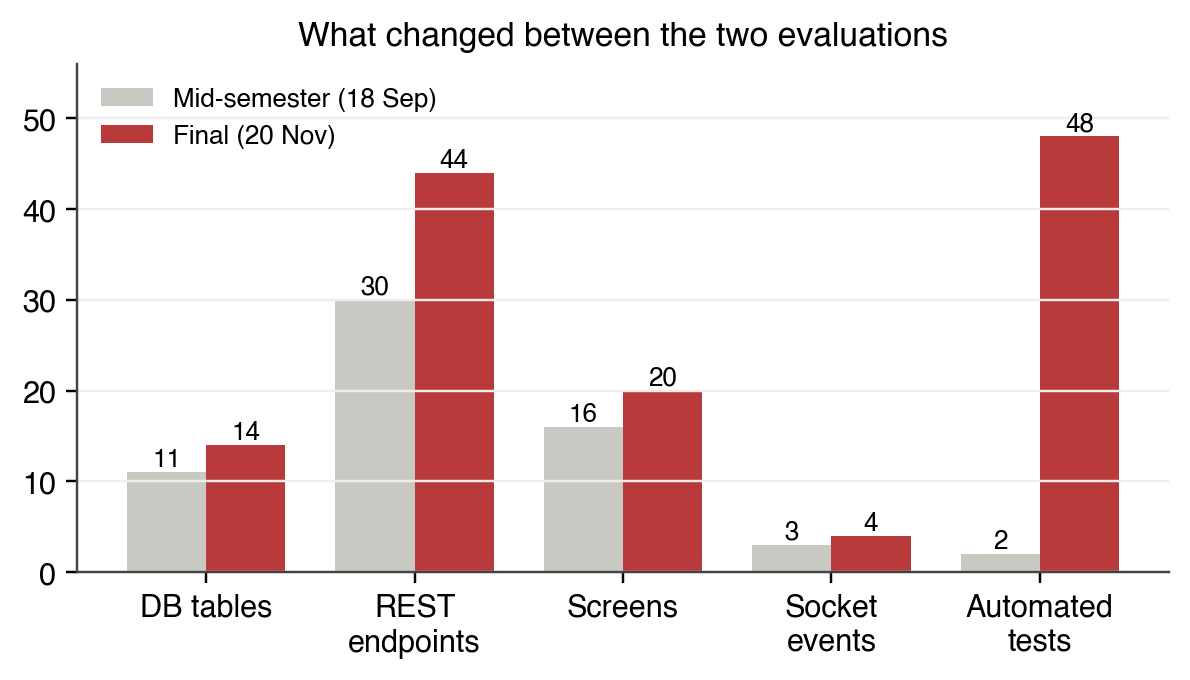
\includegraphics[width=0.92\textwidth]{figures/charts/chart-mid-vs-final.png}
\caption{The system at the two evaluations}
\label{fig:midfinal}
\end{figure}

\begin{figure}[htbp]
\centering
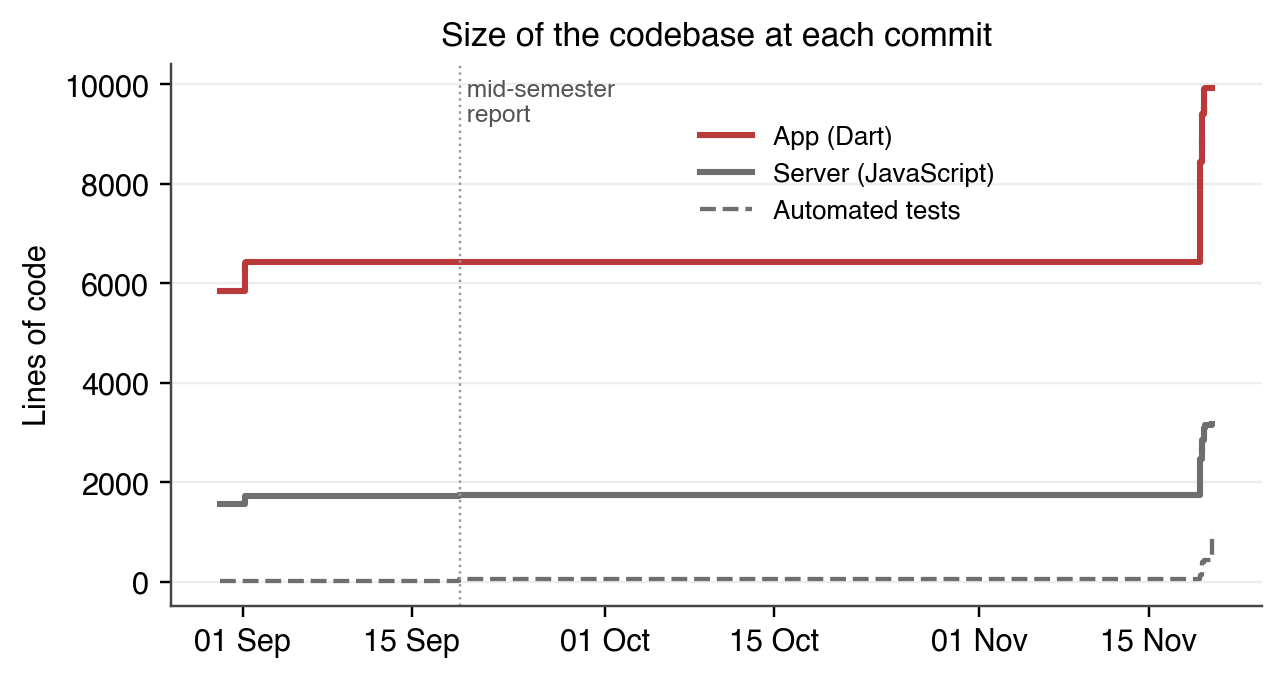
\includegraphics[width=0.92\textwidth]{figures/charts/chart-code-growth.png}
\caption{Lines of code at each commit in the local repository}
\label{fig:growth}
\end{figure}

Figure~\ref{fig:midfinal} puts the two evaluations side by side. The largest relative change
is in tests, from 2 to 48. Figure~\ref{fig:growth} counts lines at every commit. The flat
stretch between mid-semester and 19 November is an honest picture of the repository rather
than of the work: the application code was committed in bursts, and the features from
Chapter~3's Modules 8 to 14 arrived in 26 commits on 19 November. The test suite and the
report followed on 20 November. Committing more often, in smaller pieces, would have made
both the history and the journal in Chapter~\ref{ch:journal} easier to reconstruct.

\section{Summary of Findings}

\begin{itemize}
  \item The server is fast enough by a wide margin. Ordinary reads take 1 to 3~ms and one
        process handles about 2{,}600 requests a second.
  \item Discover's cost grows in a straight line with the number of activities, and the
        response size, not the query time, is what will hurt first. Pagination is the fix.
  \item 48 automated tests pass, and writing them found three defects of their own kind: a
        setup script that had never worked on a clean install, and two tests that would have
        given false confidence.
  \item Usage outcomes (time to a confirmed companion, fill rate) remain unmeasured because
        the pilot was not run.
\end{itemize}


% ===== CHAPTER 7: UML MODELS =====

\chapter{UML Models}
\label{ch:uml}

The models in this chapter were derived from the code base, not from an intended design,
using the notation of the Unified Modeling Language~\cite{booch2005,fowler2004}. The use
case, class and activity diagrams were first drawn for the mid-semester report; the use case
and domain class diagrams have been redrawn for the final system. The sequence,
communication, state, component and deployment diagrams in
Sections~\ref{sec:seq} to~\ref{sec:deploy} are new. They were rendered with
PlantUML~\cite{plantuml2026} and the sources are kept in \texttt{figures/} beside this
report, so every figure can be regenerated when the implementation moves.

\section{Use Case Diagram and Scenarios}

\subsection{Use Case Diagram}

Figure~\ref{fig:usecase} shows the system boundary, the actors and thirty-two use
cases grouped into four areas. UC22 to UC32 were added after mid-semester. The primary actor is a \emph{Student}, specialised into
the two roles a student takes within a given activity. Those roles are per-activity and
not per-account: the same student is the Host of an activity they posted and a
Participant in one they joined, often on the same afternoon.

\begin{figure}[htbp]
\centering
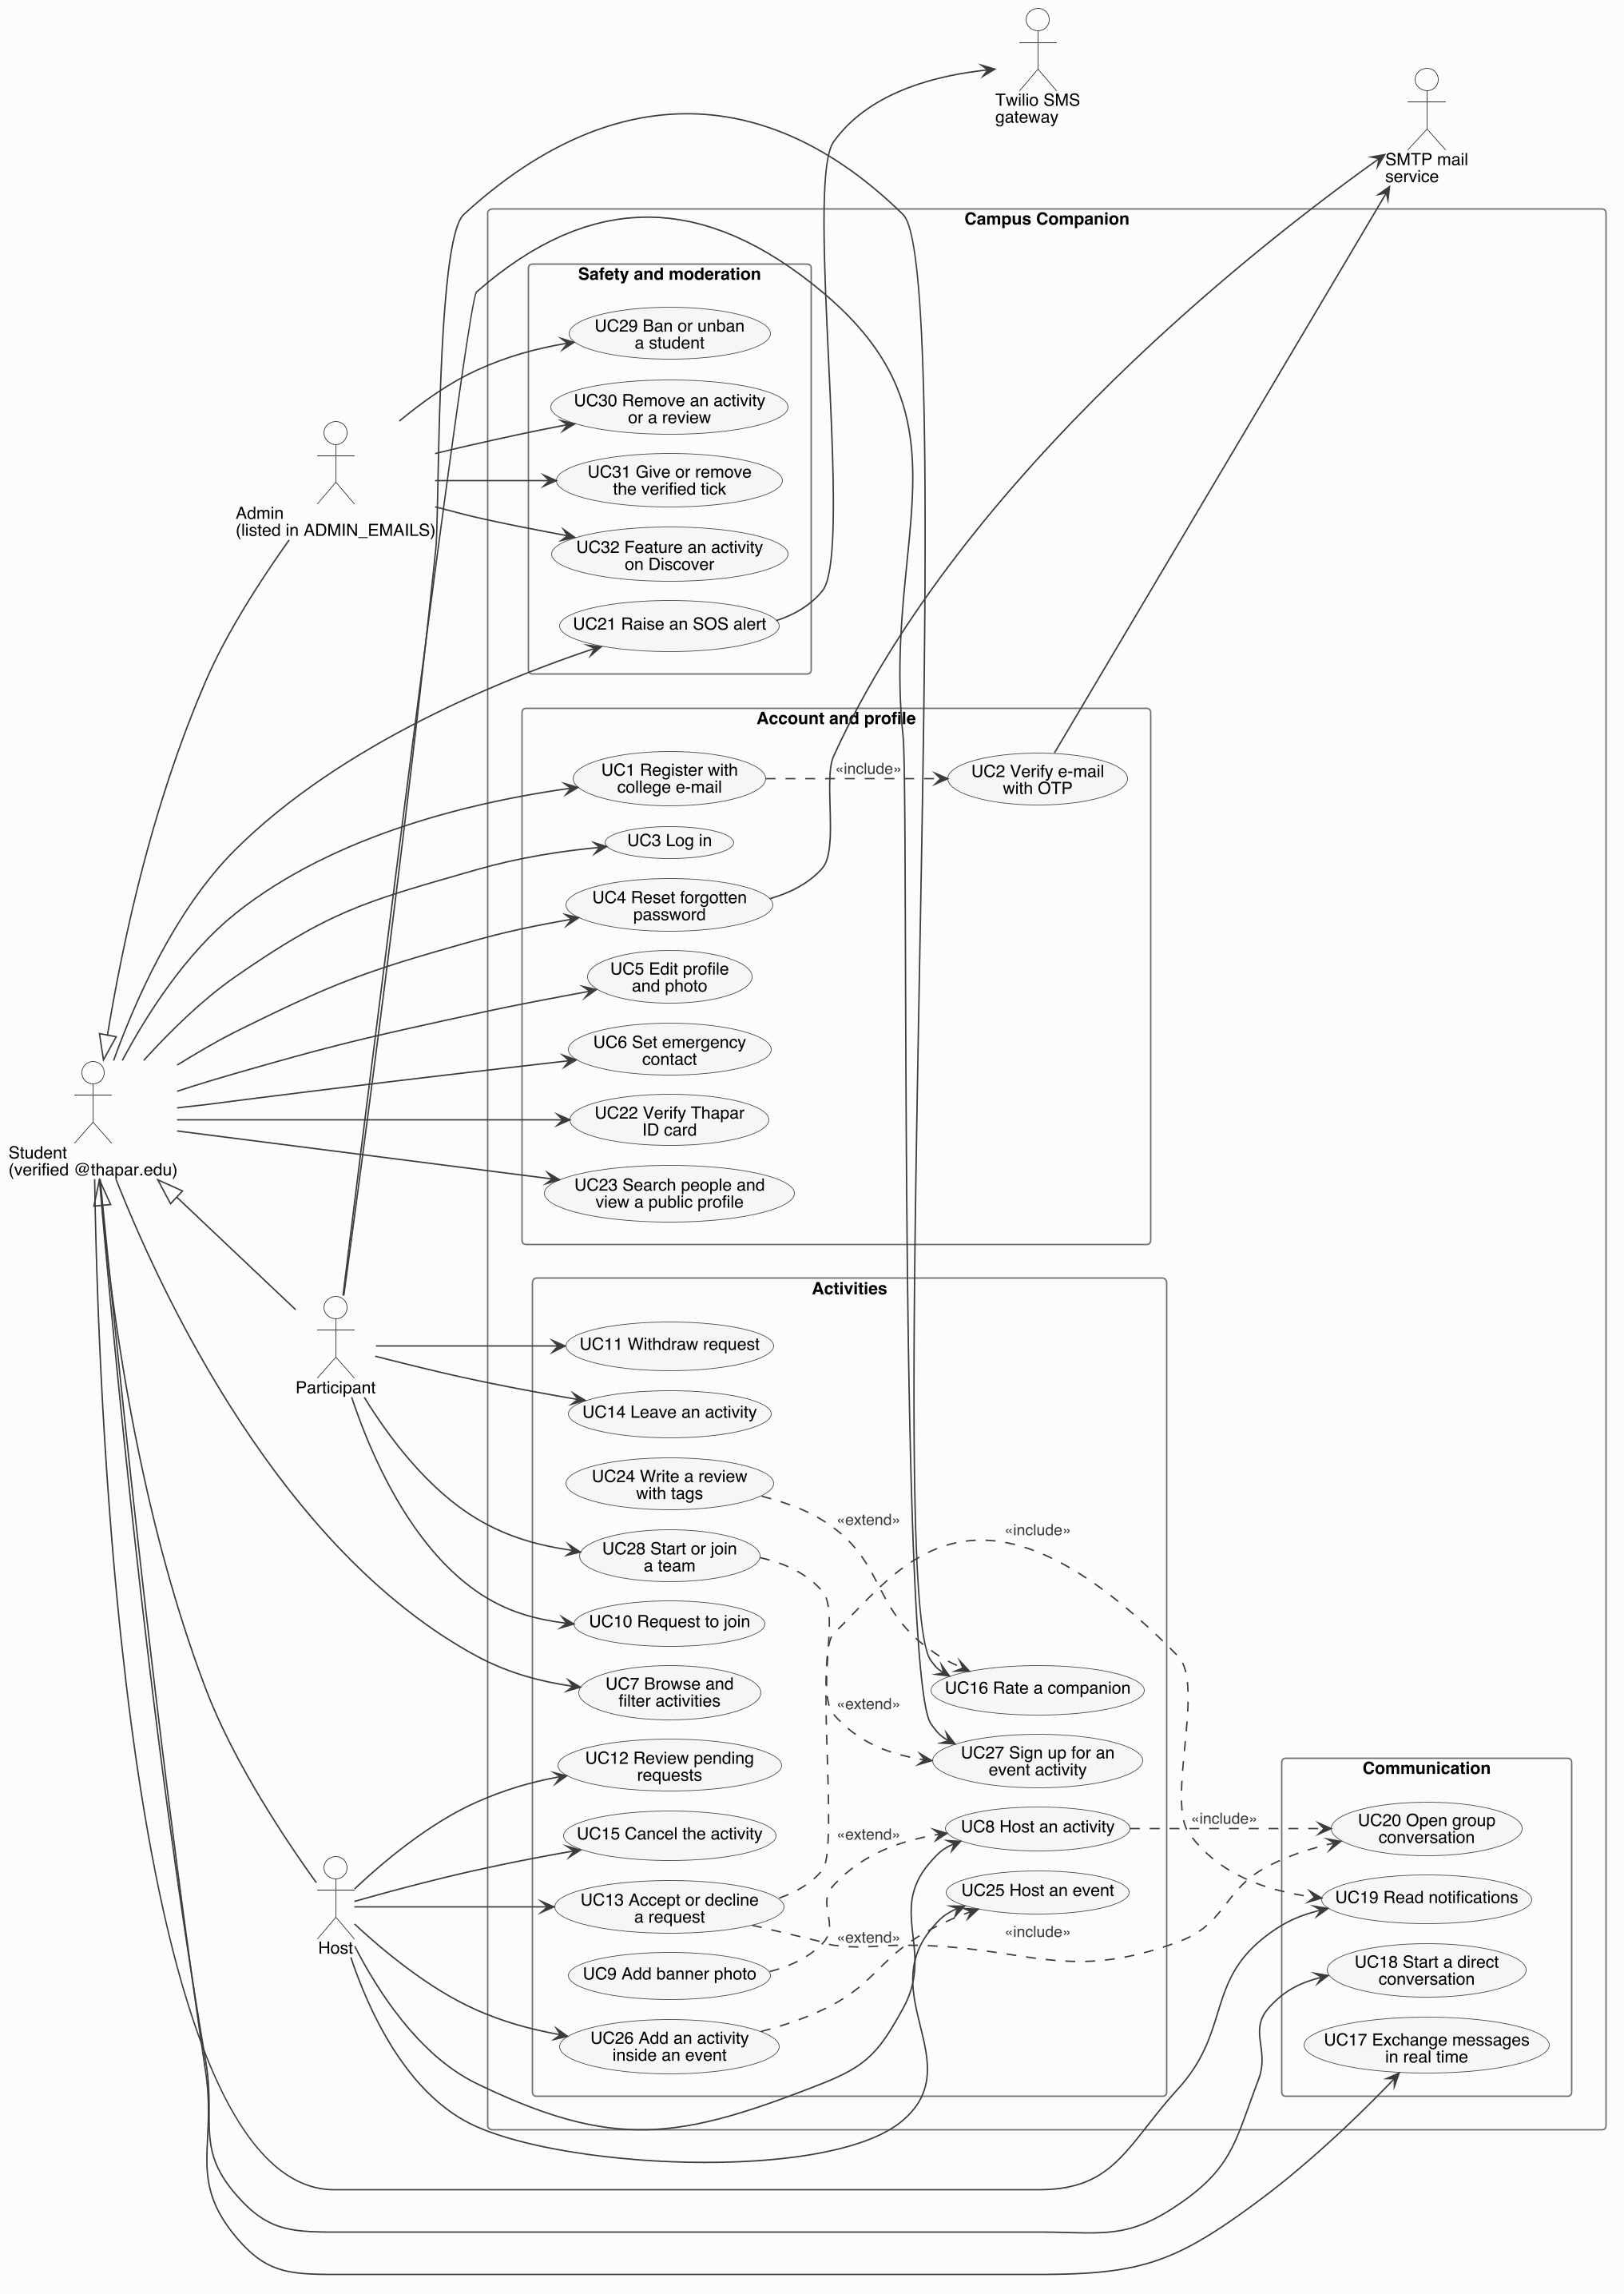
\includegraphics[width=\textwidth]{figures/usecase.png}
\caption{Use case diagram of Campus Companion at the final evaluation}
\label{fig:usecase}
\end{figure}

\subsection{Actors}

\begin{itemize}[nosep]
  \item \textbf{Student:} anyone holding a verified \texttt{@thapar.edu} account. Every
        other human actor is a student in a particular role.
  \item \textbf{Host:} the role a student occupies for an activity they created. Only
        the host may review requests, accept or decline them, set the banner, or cancel
        the activity.
  \item \textbf{Participant:} the role a student occupies for an activity they were
        admitted to. Only a participant may leave an activity or rate the people in it.
  \item \textbf{SMTP mail service:} the external mail relay that delivers verification
        and password-reset codes.
  \item \textbf{Twilio SMS gateway:} the external gateway that delivers the SOS message
        to an emergency contact.
  \item \textbf{Admin:} a student whose address is listed in the server's
        \texttt{ADMIN\_EMAILS} setting, with the moderation use cases UC29 to UC32.
\end{itemize}

\subsection{Use Case Scenarios}

\paragraph{UC1: Register with college e-mail}
\textbf{Precondition} The student has an \texttt{@thapar.edu} address and no verified
account on it.\\
\textbf{Main flow}
\begin{enumerate}[nosep]
  \item The student supplies name, e-mail, password and gender.
  \item The application rejects a non-institutional address before sending anything.
  \item The server re-checks the domain, hashes the password with bcrypt, and writes an
        unverified user row.
  \item The server issues a six-digit code valid for ten minutes and mails it.
  \item The student enters the code; the server marks the account verified and deletes
        the code.
\end{enumerate}
\textbf{Alternative flows} \emph{3a.} A verified account already exists: 409, and the
student is sent to log in. \emph{3b.} An unverified row exists: it is reused and a fresh
code is sent. \emph{5a.} The code is wrong or expired: the student may request a resend,
subject to a sixty-second cooldown.\\
\textbf{Postcondition} A verified account exists and can be used to log in.

\paragraph{UC8: Host an activity}
\textbf{Precondition} A valid session exists.\\
\textbf{Main flow}
\begin{enumerate}[nosep]
  \item The student opens the host flow from the centre button or the home card.
  \item They enter title, category, date, time, optional duration, capacity and landmark.
  \item In one transaction the server inserts the activity, enrols the host as its first
        participant, creates the conversation and adds the host to it.
  \item The activity appears immediately in Discover and on the host's home screen.
\end{enumerate}
\textbf{Alternative flow} \emph{3a.} Any statement fails: the whole transaction rolls
back and no partial activity is left behind.\\
\textbf{Extension} \emph{UC9.} A banner photo is uploaded afterwards; a failure here
leaves the activity intact and is reported as a photo failure only.\\
\textbf{Postcondition} An activity exists with its host enrolled and its group
conversation open.

\paragraph{UC10: Request to join}
\textbf{Precondition} A valid session exists and the student is not the host.\\
\textbf{Main flow}
\begin{enumerate}[nosep]
  \item The student opens an activity from Discover and taps \emph{Request to join}.
  \item The server confirms they are neither the host nor already a participant, that
        the activity is not full, and that they were not previously declined.
  \item A pending request row is written and the host is notified.
\end{enumerate}
\textbf{Alternative flows} \emph{2a.} Already the host or a participant: 400.
\emph{2b.} Capacity reached: 409. \emph{2c.} Previously declined for this activity: 403,
and the decision is final.\\
\textbf{Postcondition} Exactly one pending request exists for this (activity, student).

\paragraph{UC13: Accept or decline a request}
\textbf{Precondition} The caller is the host and the request is pending.\\
\textbf{Main flow}
\begin{enumerate}[nosep]
  \item The host opens the pending requests and sees each requester's name, gender and
        average rating.
  \item The host accepts or declines.
  \item The server opens a transaction and locks the activity and request rows.
  \item On acceptance it re-checks capacity, then adds the student to the participants
        and to the conversation in the same transaction.
  \item The request status and response time are recorded, the transaction commits, and
        the requester is notified either way.
\end{enumerate}
\textbf{Alternative flows} \emph{3a.} Caller is not the host: 403. \emph{3b.} The request
is no longer pending: 400. \emph{4a.} The activity filled while the request waited: 409
and full rollback.\\
\textbf{Postcondition} The request is resolved, and on acceptance the student is both a
participant and a member of the group chat.

\paragraph{UC16: Rate a companion}
\textbf{Precondition} The activity has ended and both students took part in it.\\
\textbf{Main flow}
\begin{enumerate}[nosep]
  \item The student opens the finished activity and selects a companion.
  \item They choose a score from 1 to 5 in half-star steps.
  \item The server confirms the end time has passed, that both parties are participants,
        and that the student is not rating themselves.
  \item The score is upserted on (activity, rater, rated) and the rated student is
        notified.
\end{enumerate}
\textbf{Alternative flows} \emph{3a.} The activity has not ended: 400. \emph{3b.} Either
party did not take part: 403. \emph{3c.} Self-rating: 400.\\
\textbf{Postcondition} One rating exists for that triple, and the rated student's
displayed average reflects it.

\paragraph{UC21: Raise an SOS alert}
\textbf{Precondition} A valid session exists and an emergency contact number is on file.\\
\textbf{Main flow}
\begin{enumerate}[nosep]
  \item The student triggers the SOS control.
  \item The application reads the device's coordinates and posts them.
  \item The server finds the activity the student is currently in, taken as one they
        joined that starts between one hour ago and three hours ahead.
  \item It composes a message containing a map link and the names of the other
        participants, sends it through Twilio, and records the alert.
\end{enumerate}
\textbf{Alternative flow} \emph{1a.} No emergency contact is stored: the server refuses
and says so, rather than appearing to send.\\
\textbf{Implementation status} Steps 3 to 4 are complete. Step 2 is not: the control
currently shows a placeholder message, and reading the device location is the first
task of the second half.\\
\textbf{Postcondition} The emergency contact has received a text carrying the student's
position and companions, and one row exists in \texttt{sos\_alerts}.

\section{Class Diagram}

The class model is presented in two figures. Splitting it is a readability decision
rather than a design one: drawn as a single figure, the thirty-odd classes and their
associations do not survive reduction to the width of a page.

Figure~\ref{fig:classdomain} is the domain model, which mirrors the relational schema.
Figure~\ref{fig:classlayers} is the application, showing the Flutter client, the Express
service layer and the dependencies between them, with the domain collapsed into a single
box.

\begin{sidewaysfigure}
\centering
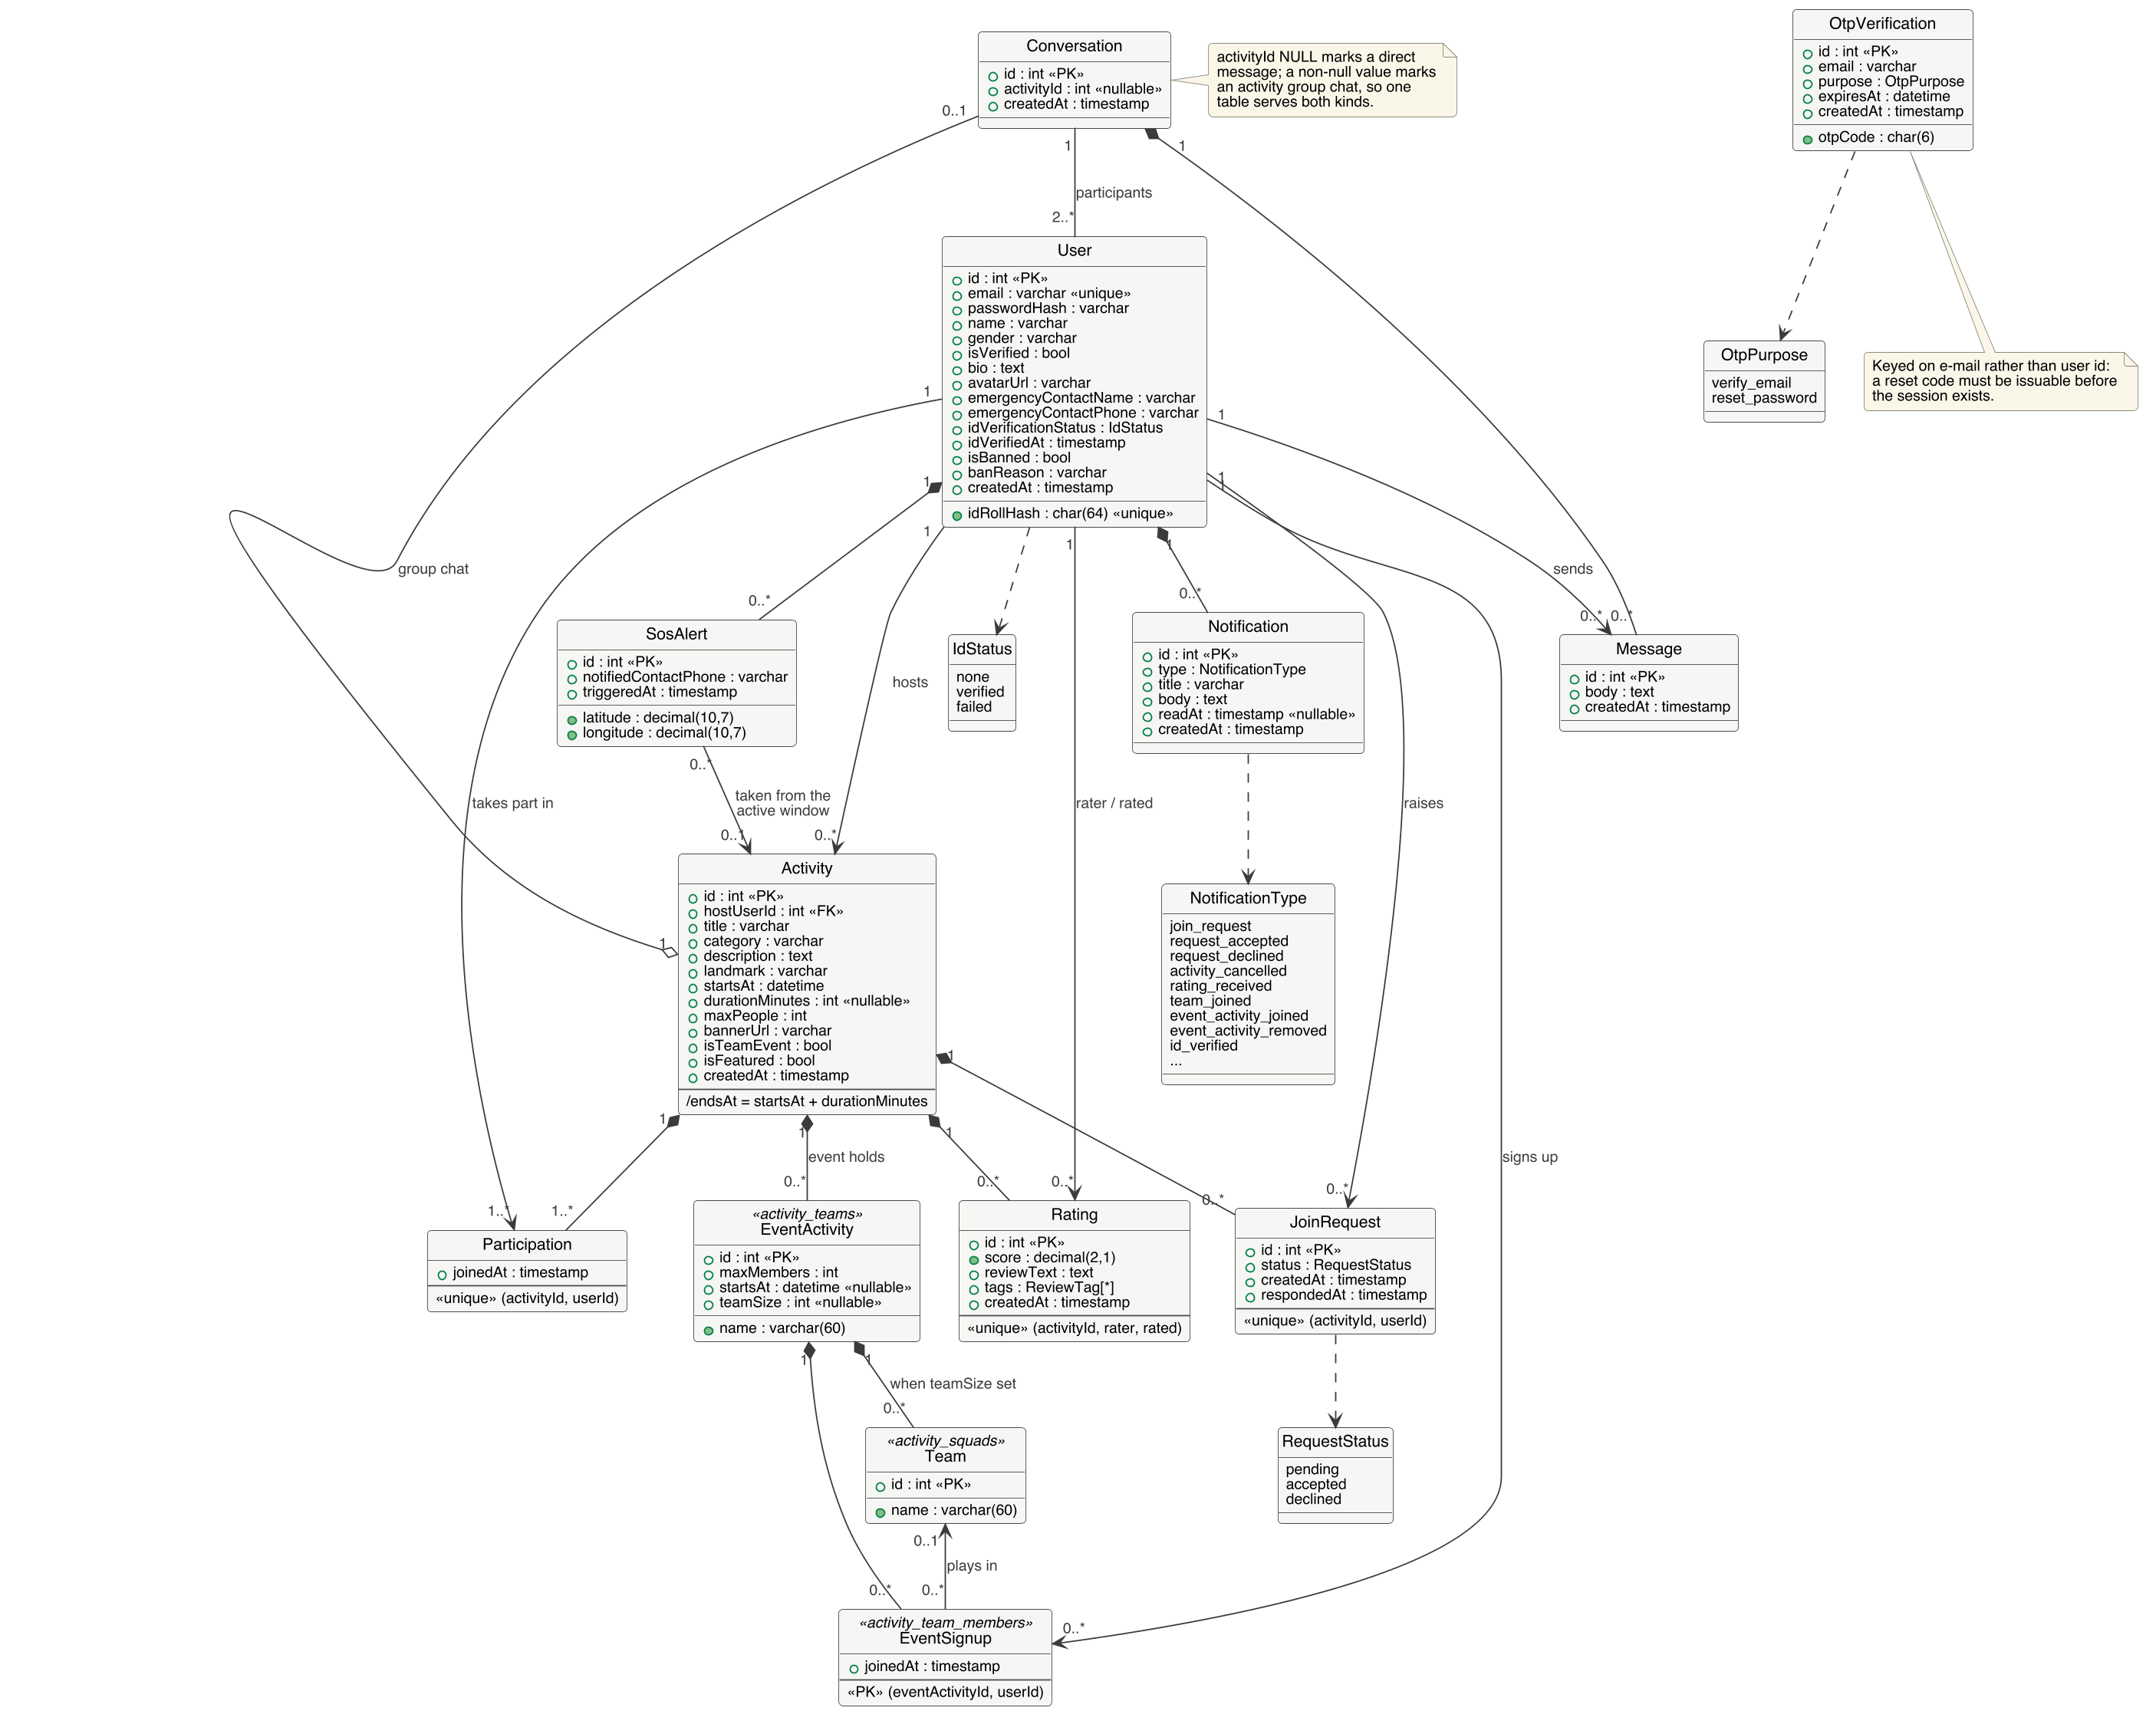
\includegraphics[width=0.94\textheight]{figures/class-domain.png}
\caption{Class diagram, part 1: the domain model and its associations}
\label{fig:classdomain}
\end{sidewaysfigure}

\begin{sidewaysfigure}
\centering
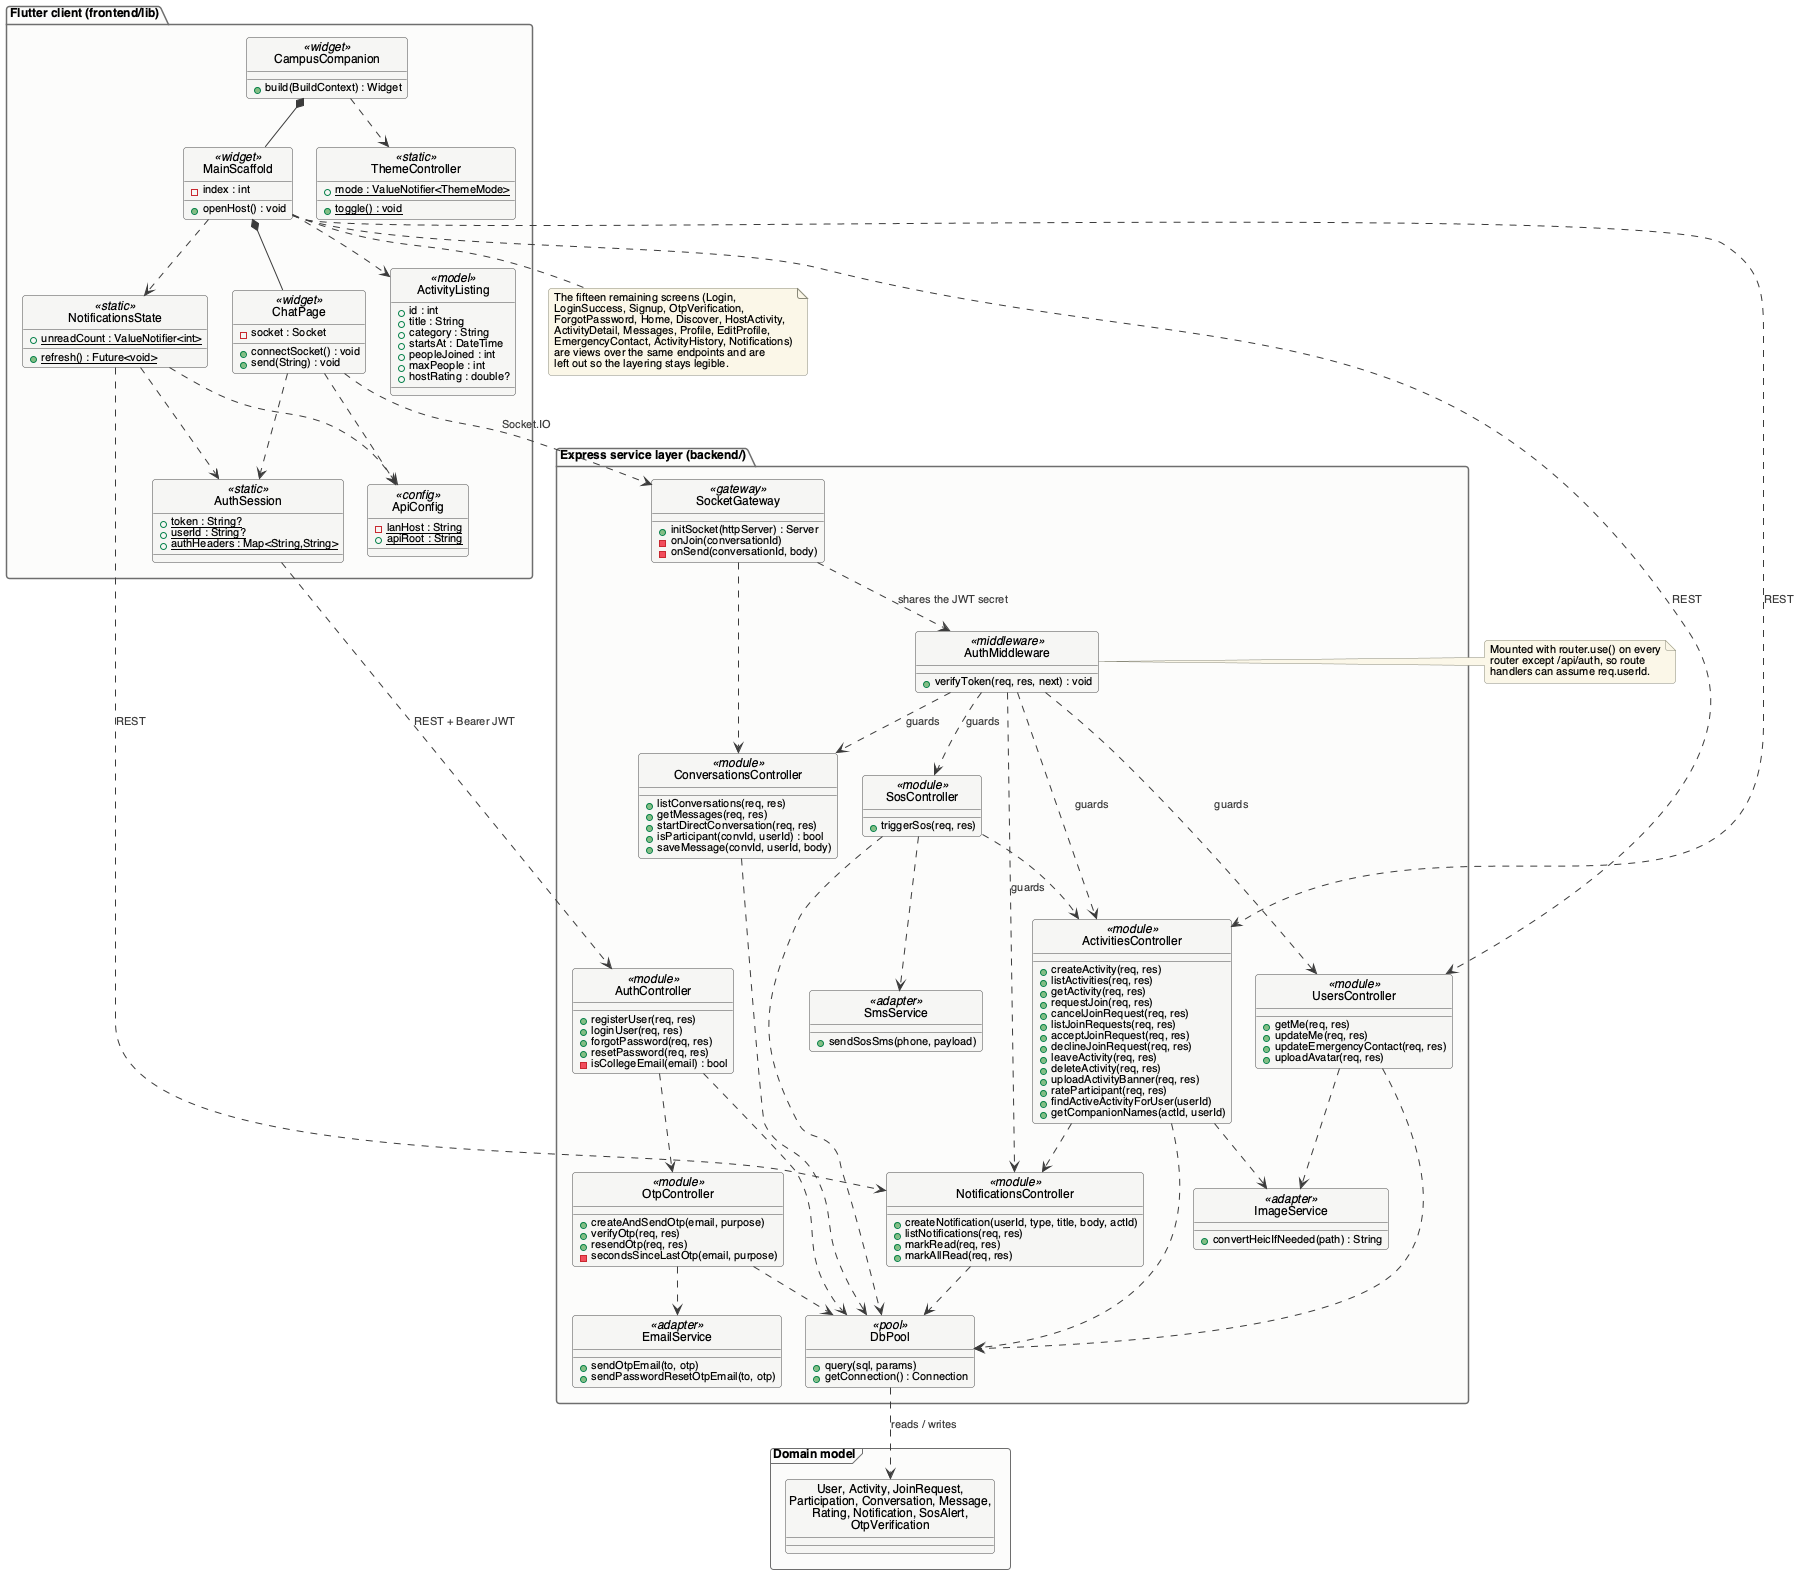
\includegraphics[width=0.94\textheight]{figures/class-layers.png}
\caption{Class diagram, part 2: the Flutter client and the Express service layer}
\label{fig:classlayers}
\end{sidewaysfigure}

\medskip
\noindent Points the diagrams are intended to make visible:

\begin{itemize}
  \item \texttt{Conversation} has a nullable link to \texttt{Activity}. That single
        nullable association is what lets group chats and direct messages share one
        table, one membership table and one message pipeline.

  \item \texttt{JoinRequest} and \texttt{Participation} are separate classes with
        separate uniqueness constraints, because a request is a negotiation that can be
        withdrawn or refused, and participation is a fact that ratings depend on.

  \item \texttt{Rating} is owned by \texttt{Activity} and points twice at \texttt{User},
        once as rater and once as rated. Its uniqueness constraint spans all three, which
        is the constraint that makes an average trustworthy.

  \item \texttt{OtpVerification} is keyed on an e-mail address rather than on a user, and
        is the only entity in the model that is not. A password-reset code has to be
        issuable before any session exists, which is exactly the situation a foreign key
        to \texttt{User} would make awkward.

  \item In the application layer, \texttt{AuthMiddleware} sits between the routers and
        every controller except authentication. The dashed \emph{guards} dependencies are
        the reason no individual handler repeats the token check.

  \item The three adapters, \texttt{EmailService}, \texttt{SmsService} and
        \texttt{ImageService}, are the only modules that reach outside the process apart
        from the database pool. Isolating them is what will let the controllers around
        them be tested without a network.
\end{itemize}

\section{Activity Diagram}

The behaviour of the system is modelled as four activity diagrams, covering the two
journeys that matter: getting an account, and getting from an idea to a rated outing.
Each is drawn with swimlanes so that it is clear which side of the network any given
step happens on, and in particular which checks are repeated on the server after the
client has already made them. Figures~\ref{fig:actregister} and~\ref{fig:actsignin}
cover account creation and access; Figures~\ref{fig:acthostjoin}
and~\ref{fig:actrespond} cover the activity lifecycle.

\begin{sidewaysfigure}
\centering
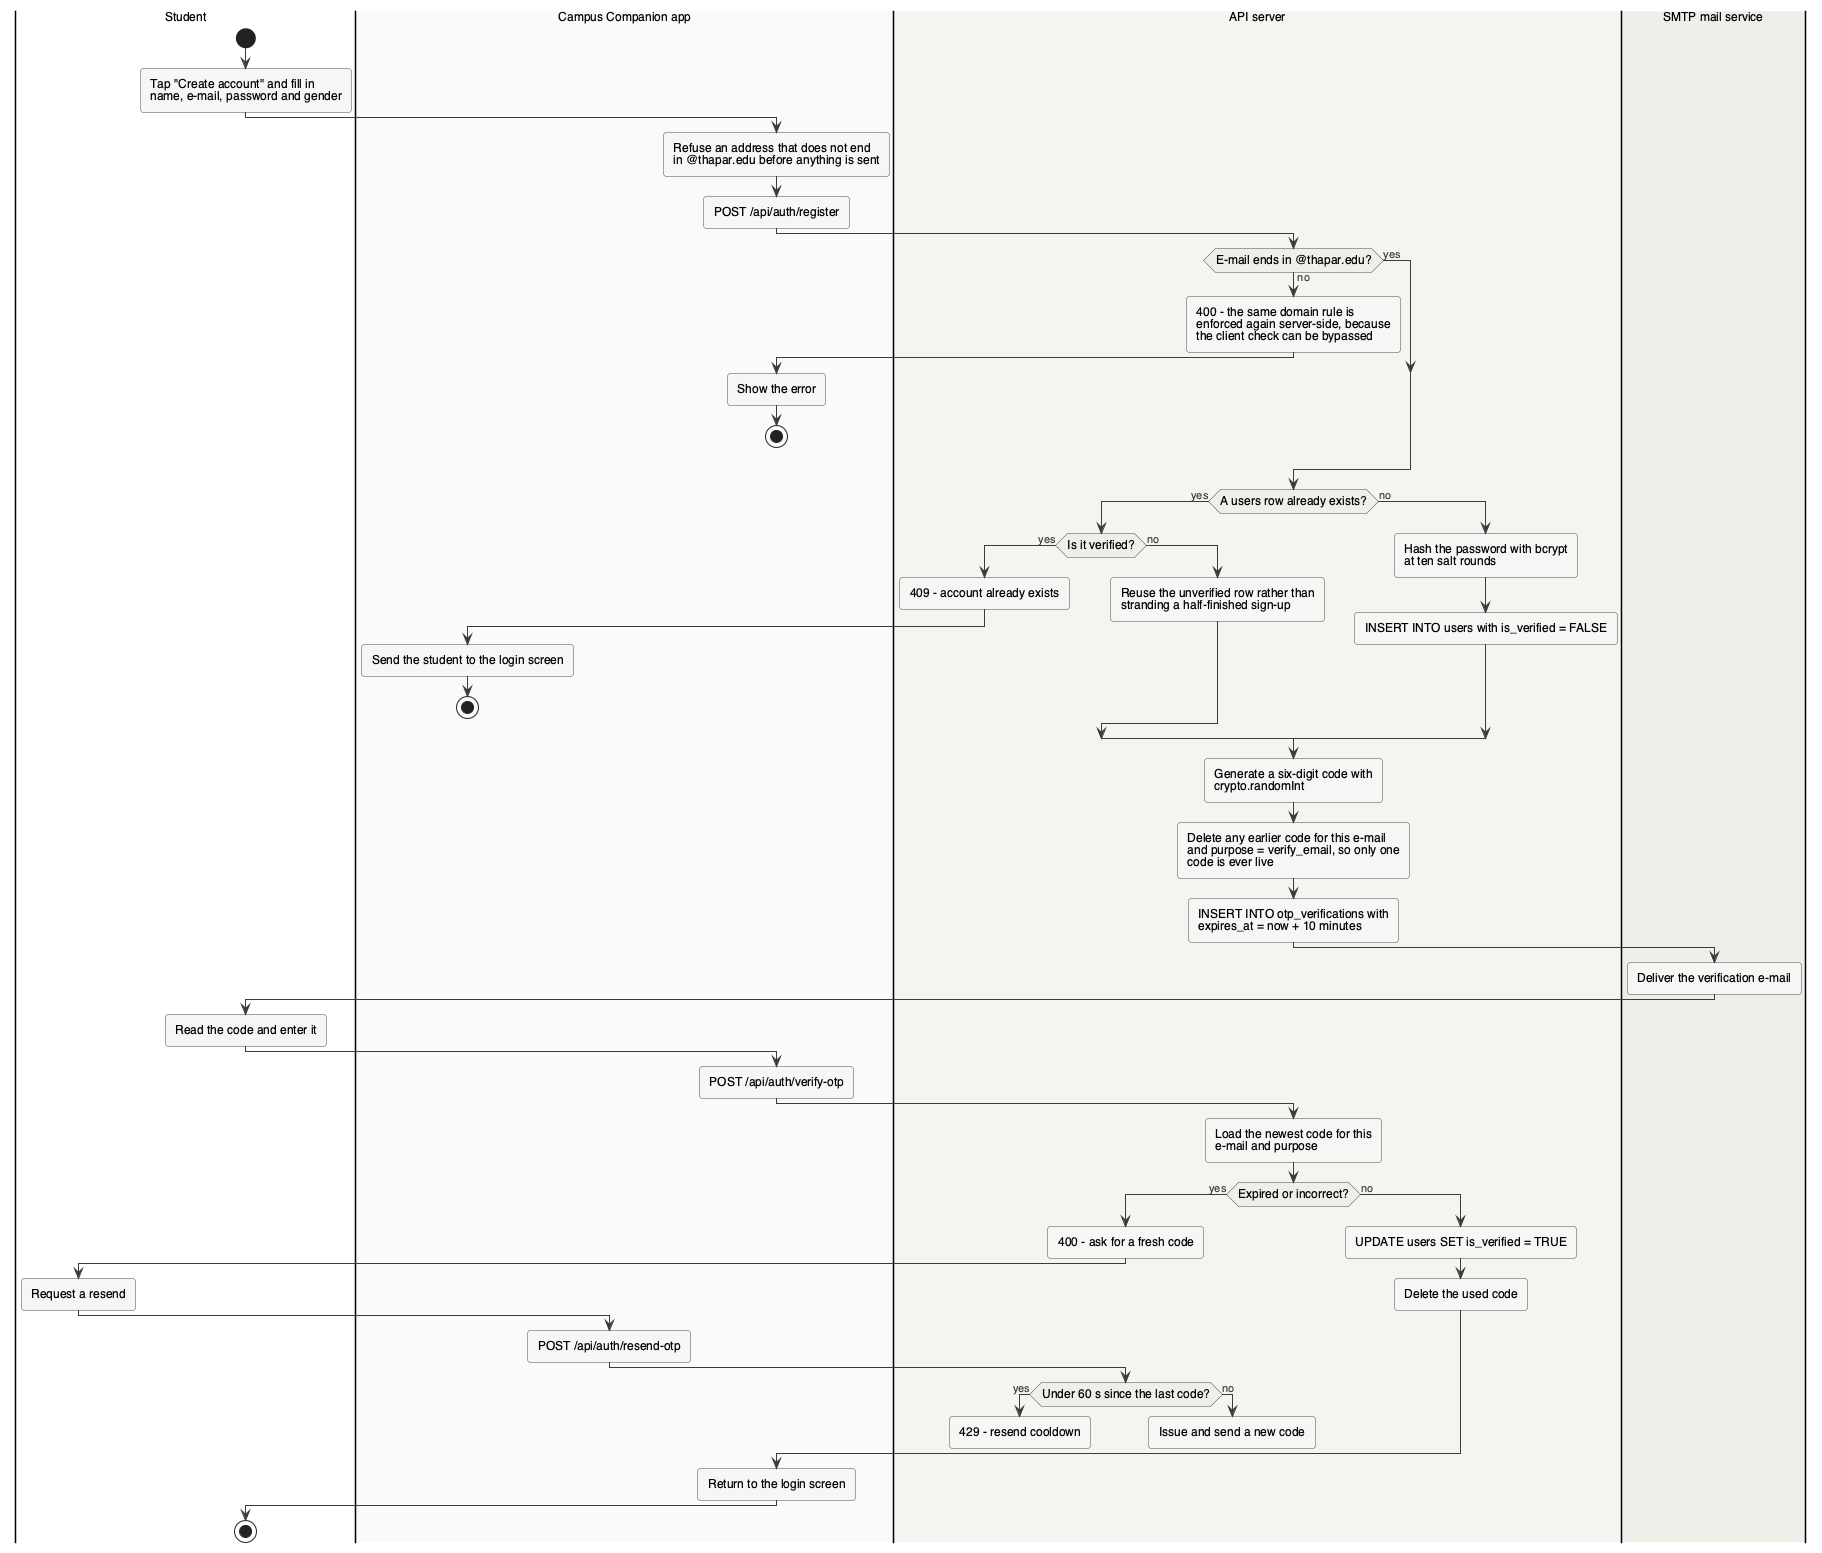
\includegraphics[width=0.90\textheight]{figures/activity-register.png}
\caption{Activity diagram, part 1: registration and e-mail verification}
\label{fig:actregister}
\end{sidewaysfigure}

\begin{figure}[htbp]
\centering
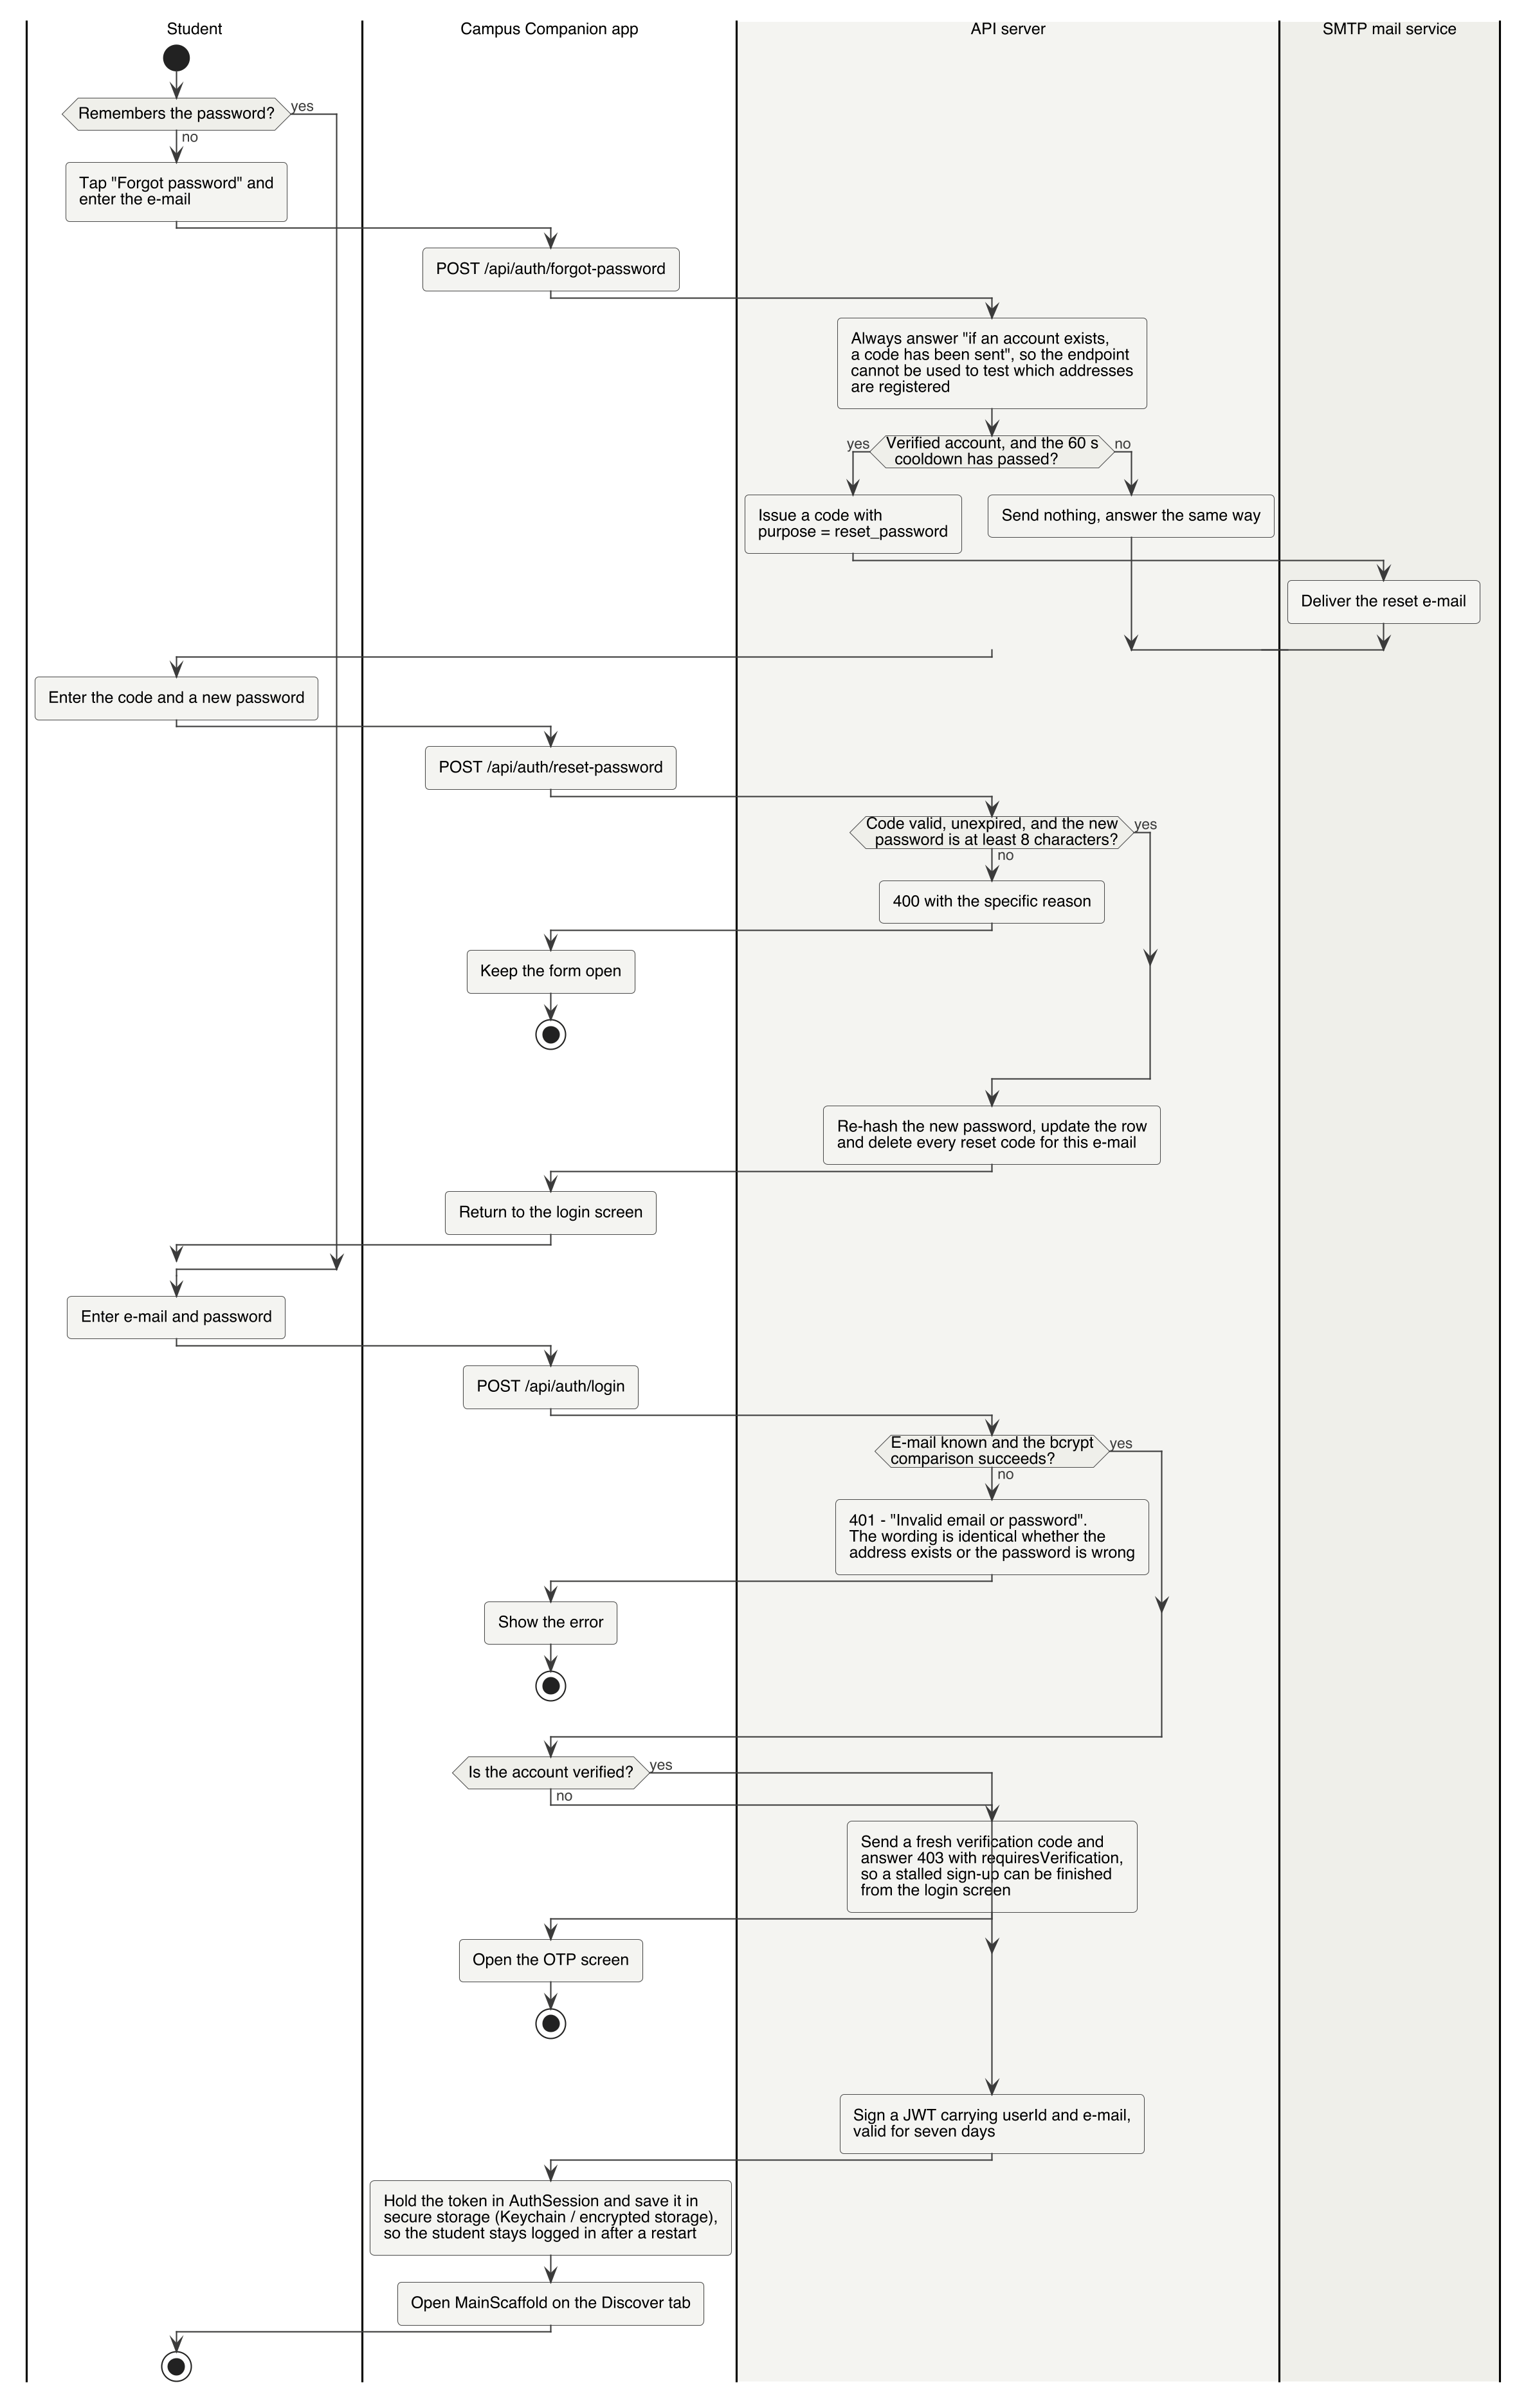
\includegraphics[height=0.90\textheight]{figures/activity-signin.png}
\caption{Activity diagram, part 2: sign-in and password recovery}
\label{fig:actsignin}
\end{figure}


\begin{figure}[htbp]
\centering
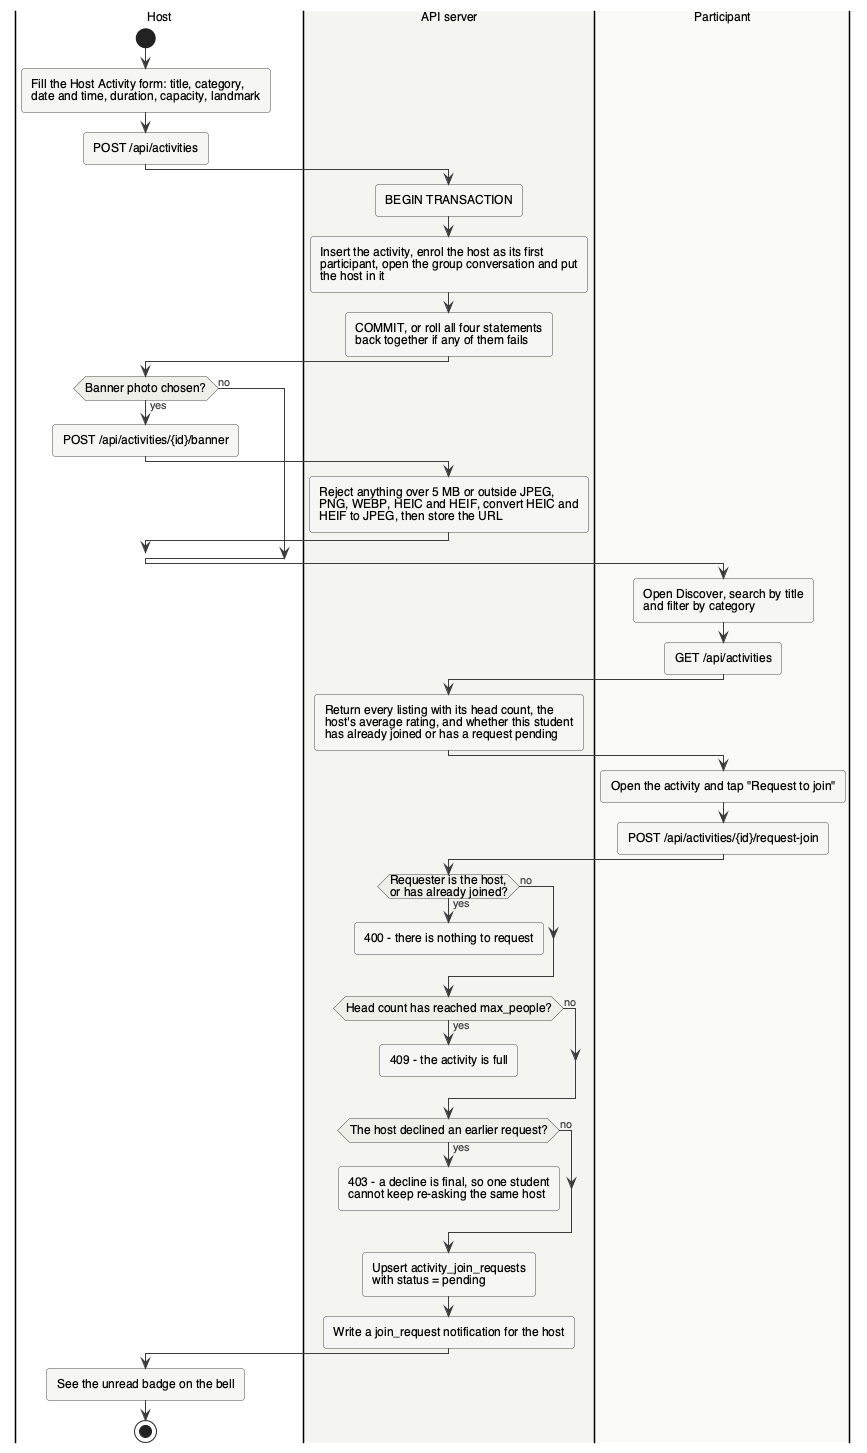
\includegraphics[height=0.90\textheight]{figures/activity-host-join.png}
\caption{Activity diagram, part 3: hosting an activity and requesting to join}
\label{fig:acthostjoin}
\end{figure}


\begin{figure}[htbp]
\centering
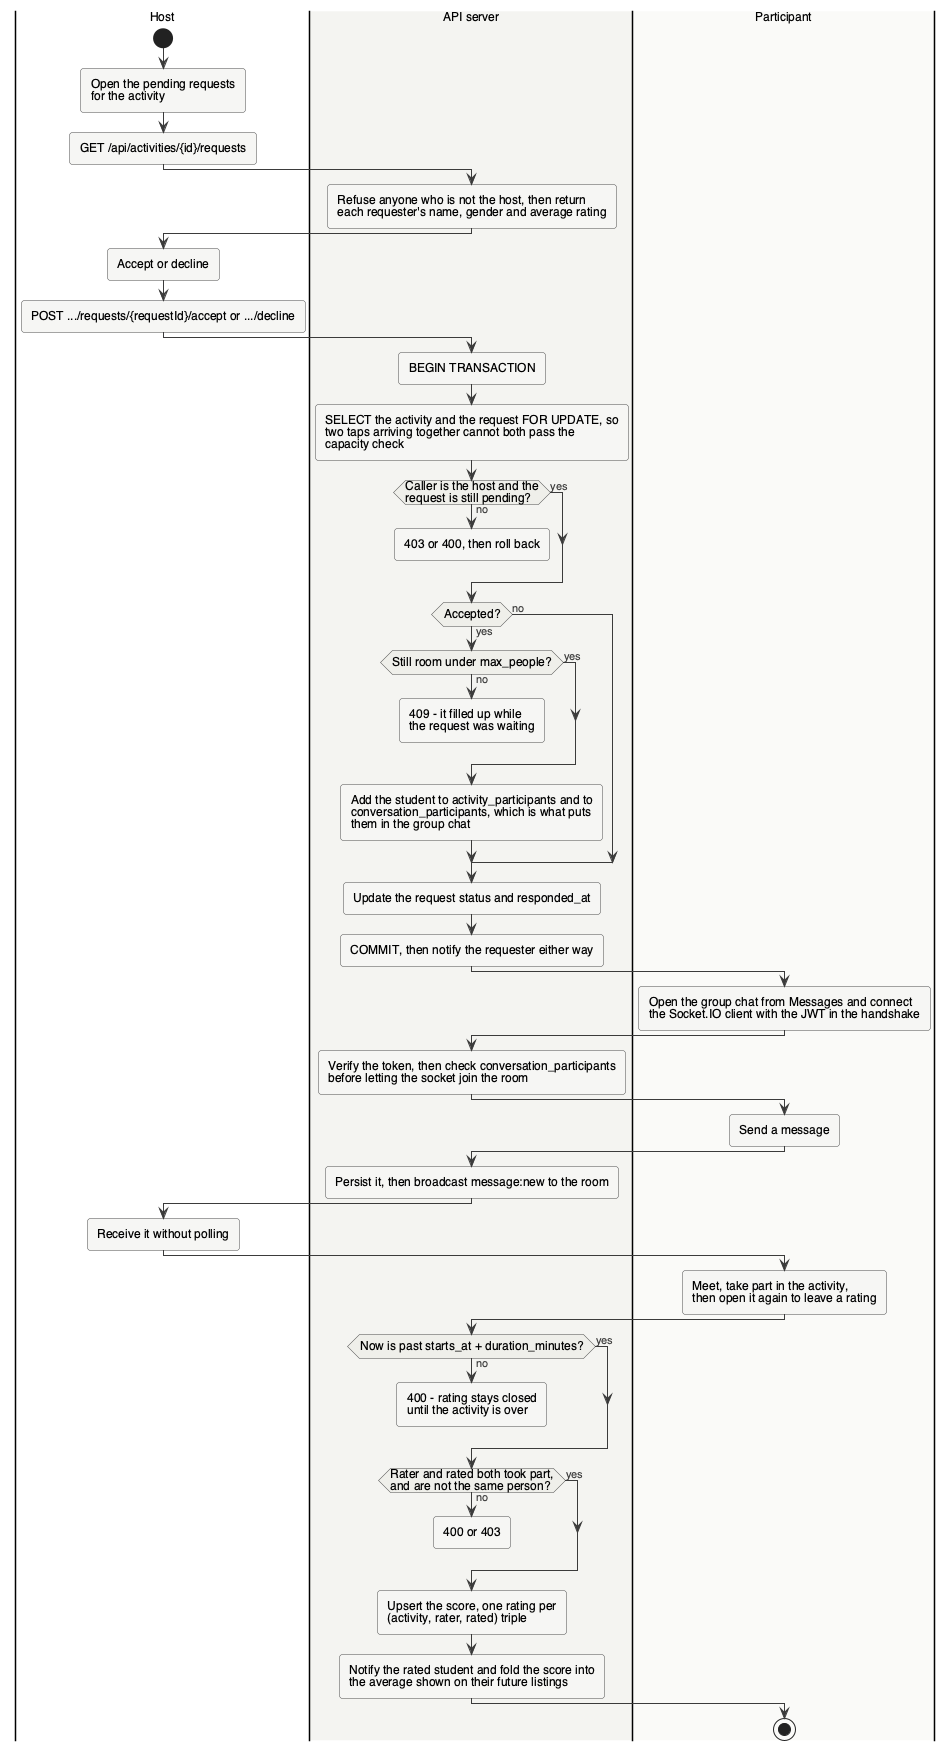
\includegraphics[height=0.90\textheight]{figures/activity-respond-rate.png}
\caption{Activity diagram, part 4: responding to a request, chatting and rating}
\label{fig:actrespond}
\end{figure}


\noindent Four aspects of the behaviour are made explicit by these diagrams and are worth
drawing attention to.

First, every rule that appears in the client lane appears again in the server lane. The
e-mail domain is checked twice, and the diagrams show both, because that duplication is
intentional rather than an oversight.

Second, the two endpoints that could leak information about who holds an account, login
and forgotten password, are drawn with their branches converging on a single identical
response. The shape of the diagram is the argument that the leak is closed.

Third, the accept path in Figure~\ref{fig:actrespond} shows the lock being taken before
the capacity check and the two inserts happening inside the same transaction. The
ordering is the whole substance of that use case, and it is the part of the system a
reader should be able to check against the code.

Fourth, the rating gate in the same figure shows that the check against
\texttt{starts\_at} plus \texttt{duration\_minutes} happens on the server. Nothing in the
client decides whether an activity is over.


\section{Sequence Diagrams}
\label{sec:seq}

Three interactions are drawn as sequence diagrams because their order is the point of them.
Figure~\ref{fig:seqjoin} follows a join request from the guest's tap to the host's accept,
including the two live notifications and the locked transaction. Figure~\ref{fig:seqid} shows
the ID card check, where the OCR and barcode reads run in parallel and the checks then stop
at the first failure. Figure~\ref{fig:seqchat} shows one chat message, which is saved before it
is broadcast.

\begin{figure}[htbp]
\centering
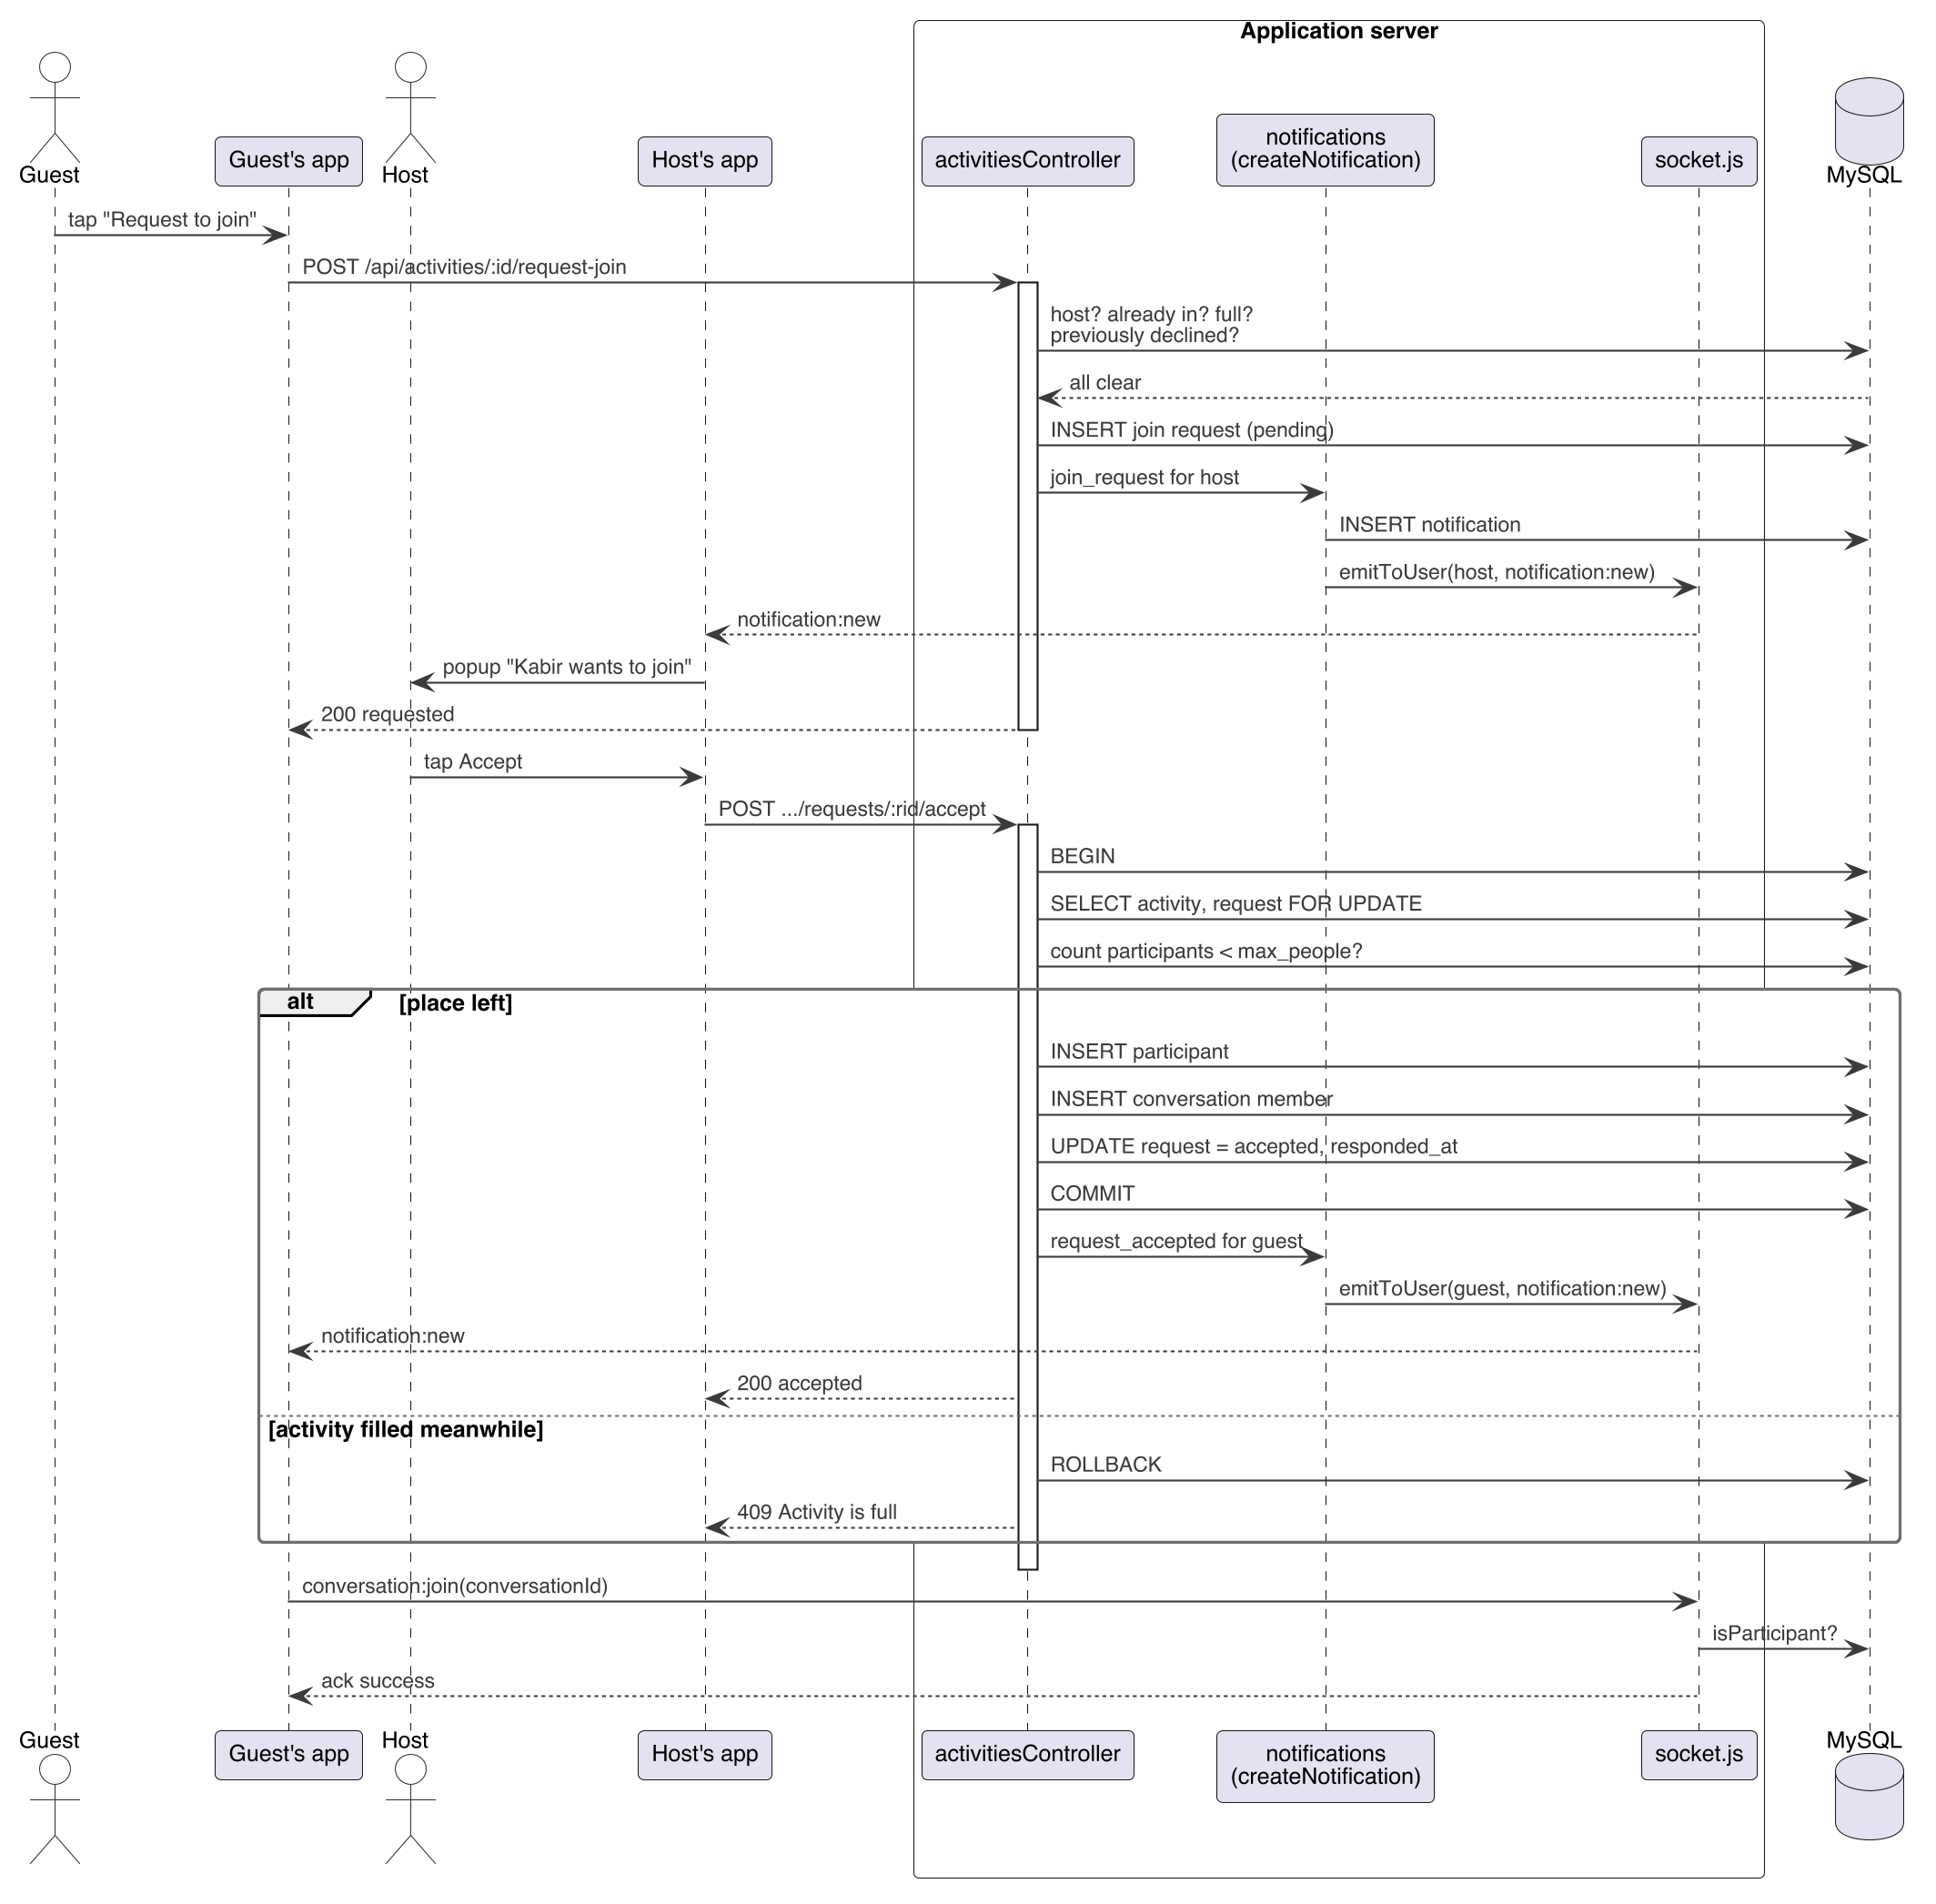
\includegraphics[width=\textwidth,height=0.86\textheight,keepaspectratio]{figures/sequence-join.png}
\caption{Sequence diagram: requesting to join and being accepted}
\label{fig:seqjoin}
\end{figure}

\begin{figure}[htbp]
\centering
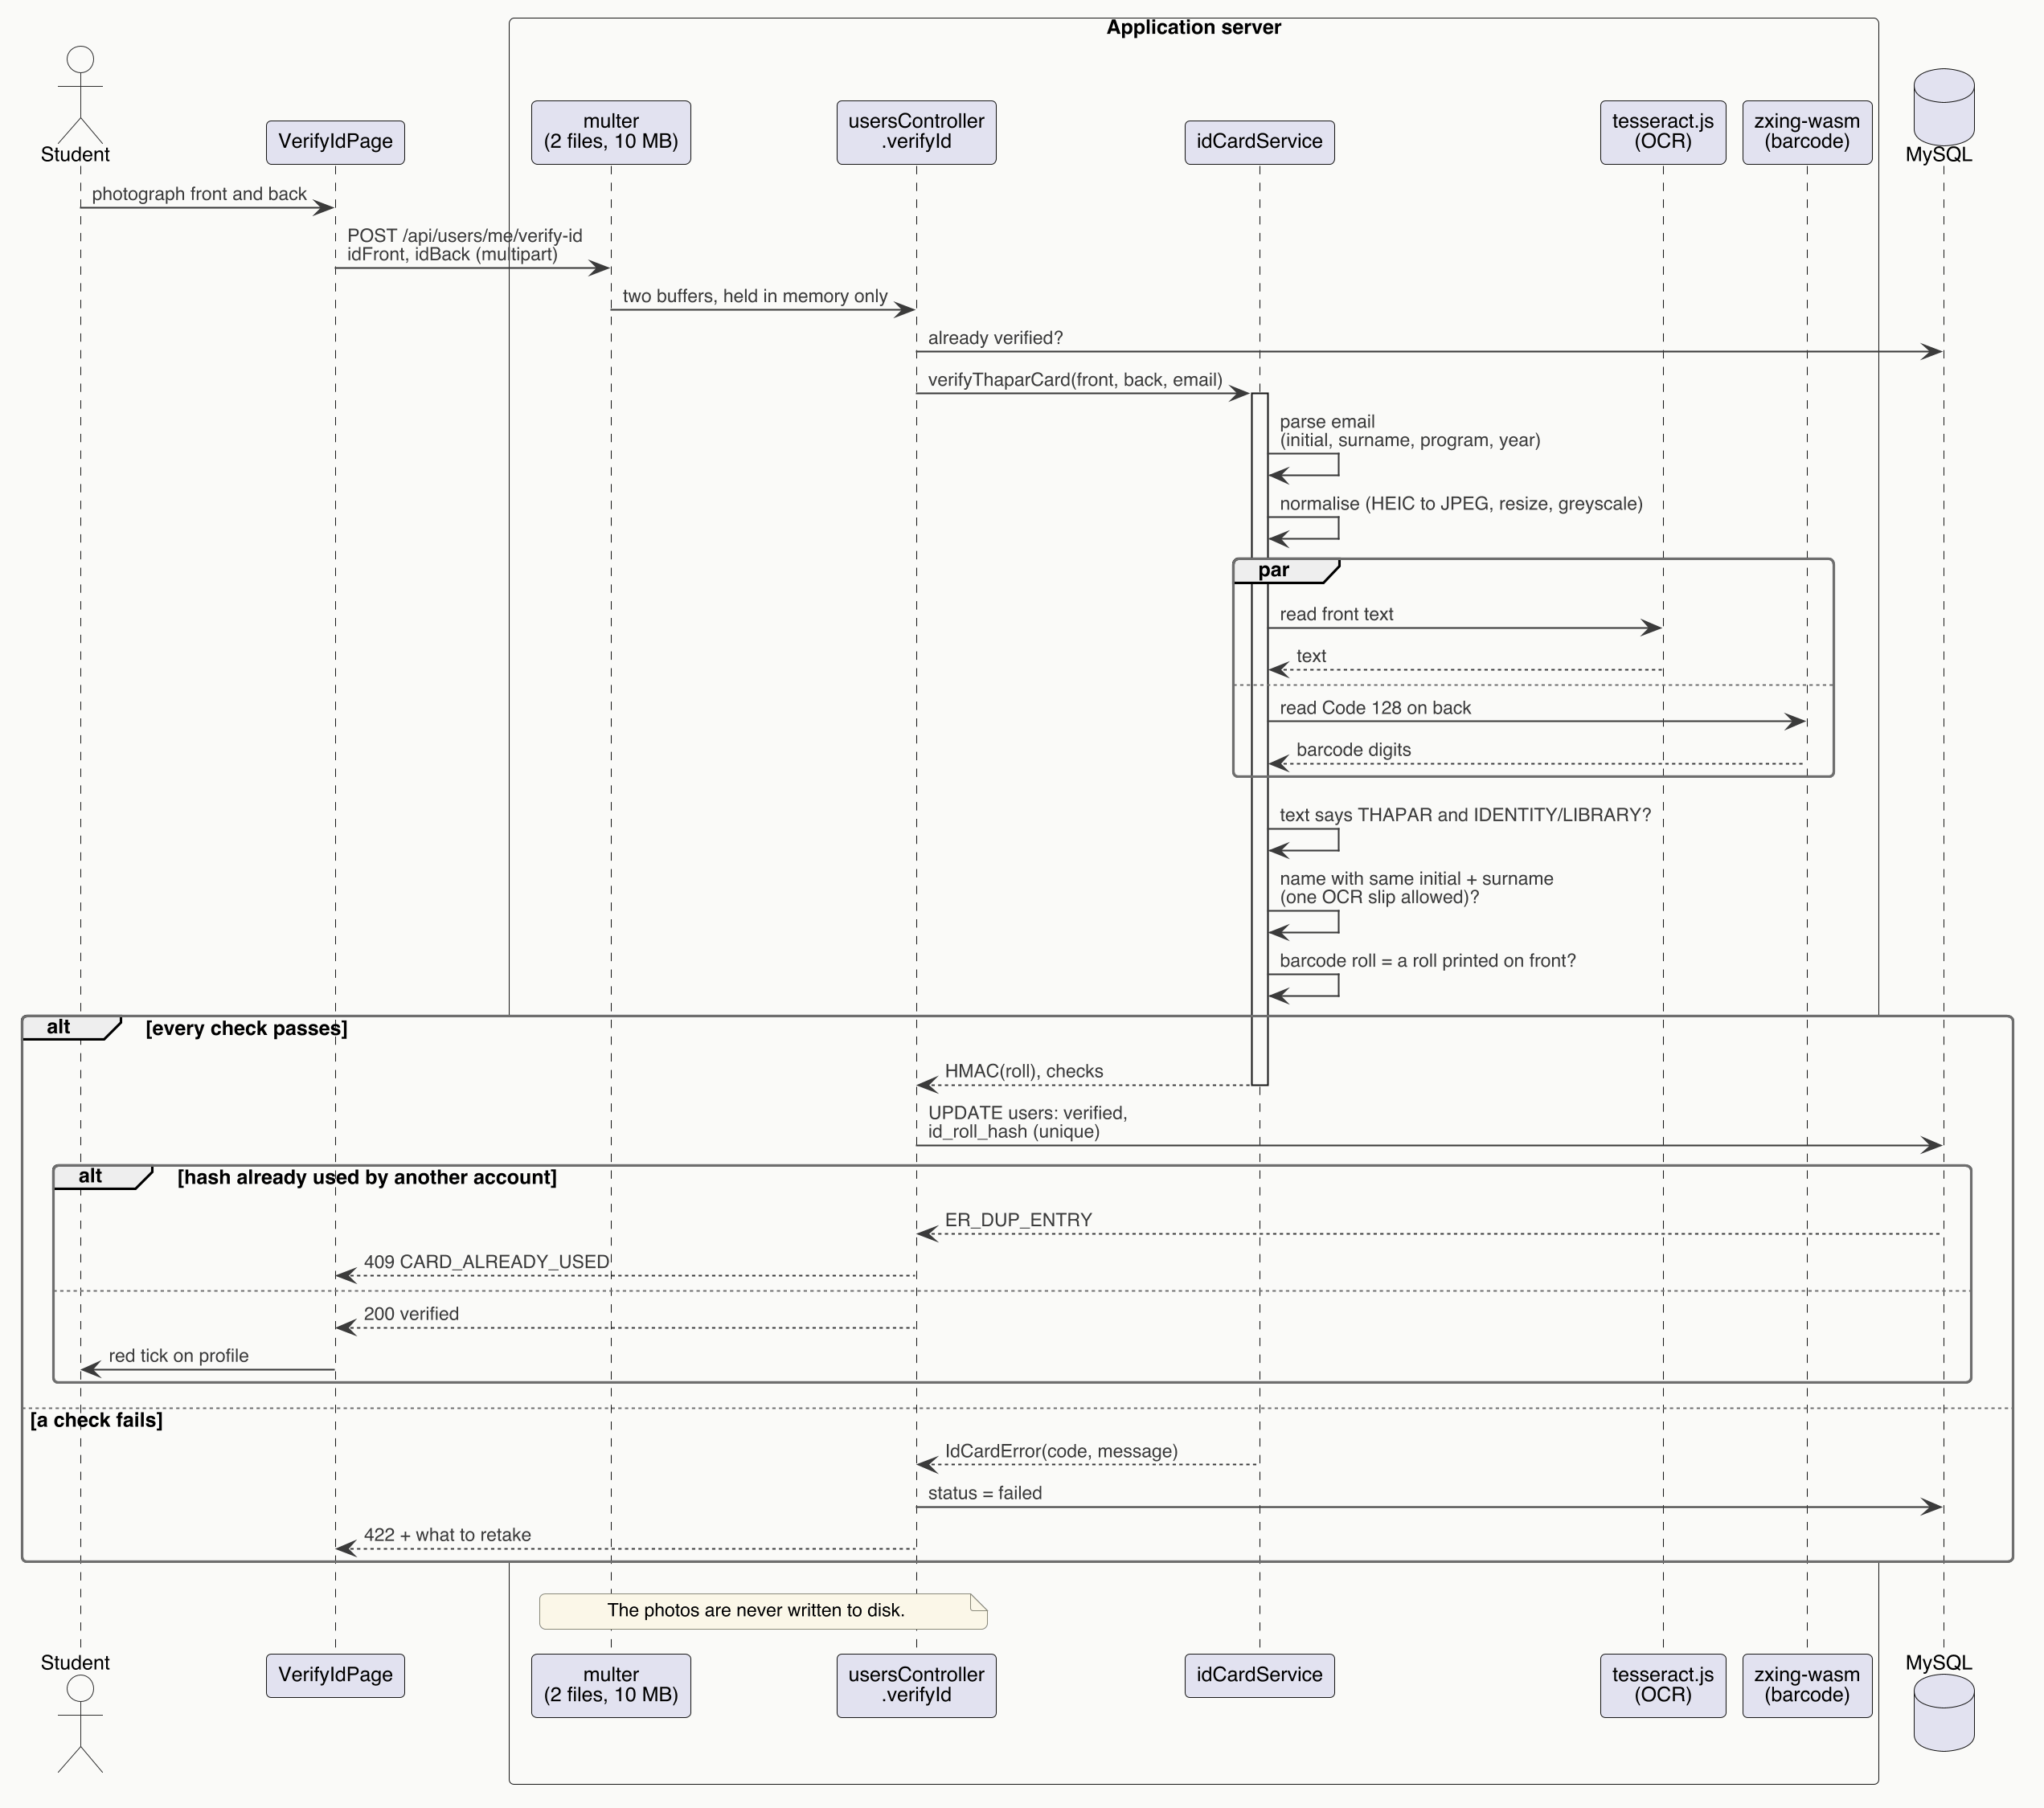
\includegraphics[width=\textwidth]{figures/sequence-idverify.png}
\caption{Sequence diagram: checking a Thapar ID card}
\label{fig:seqid}
\end{figure}

\begin{figure}[htbp]
\centering
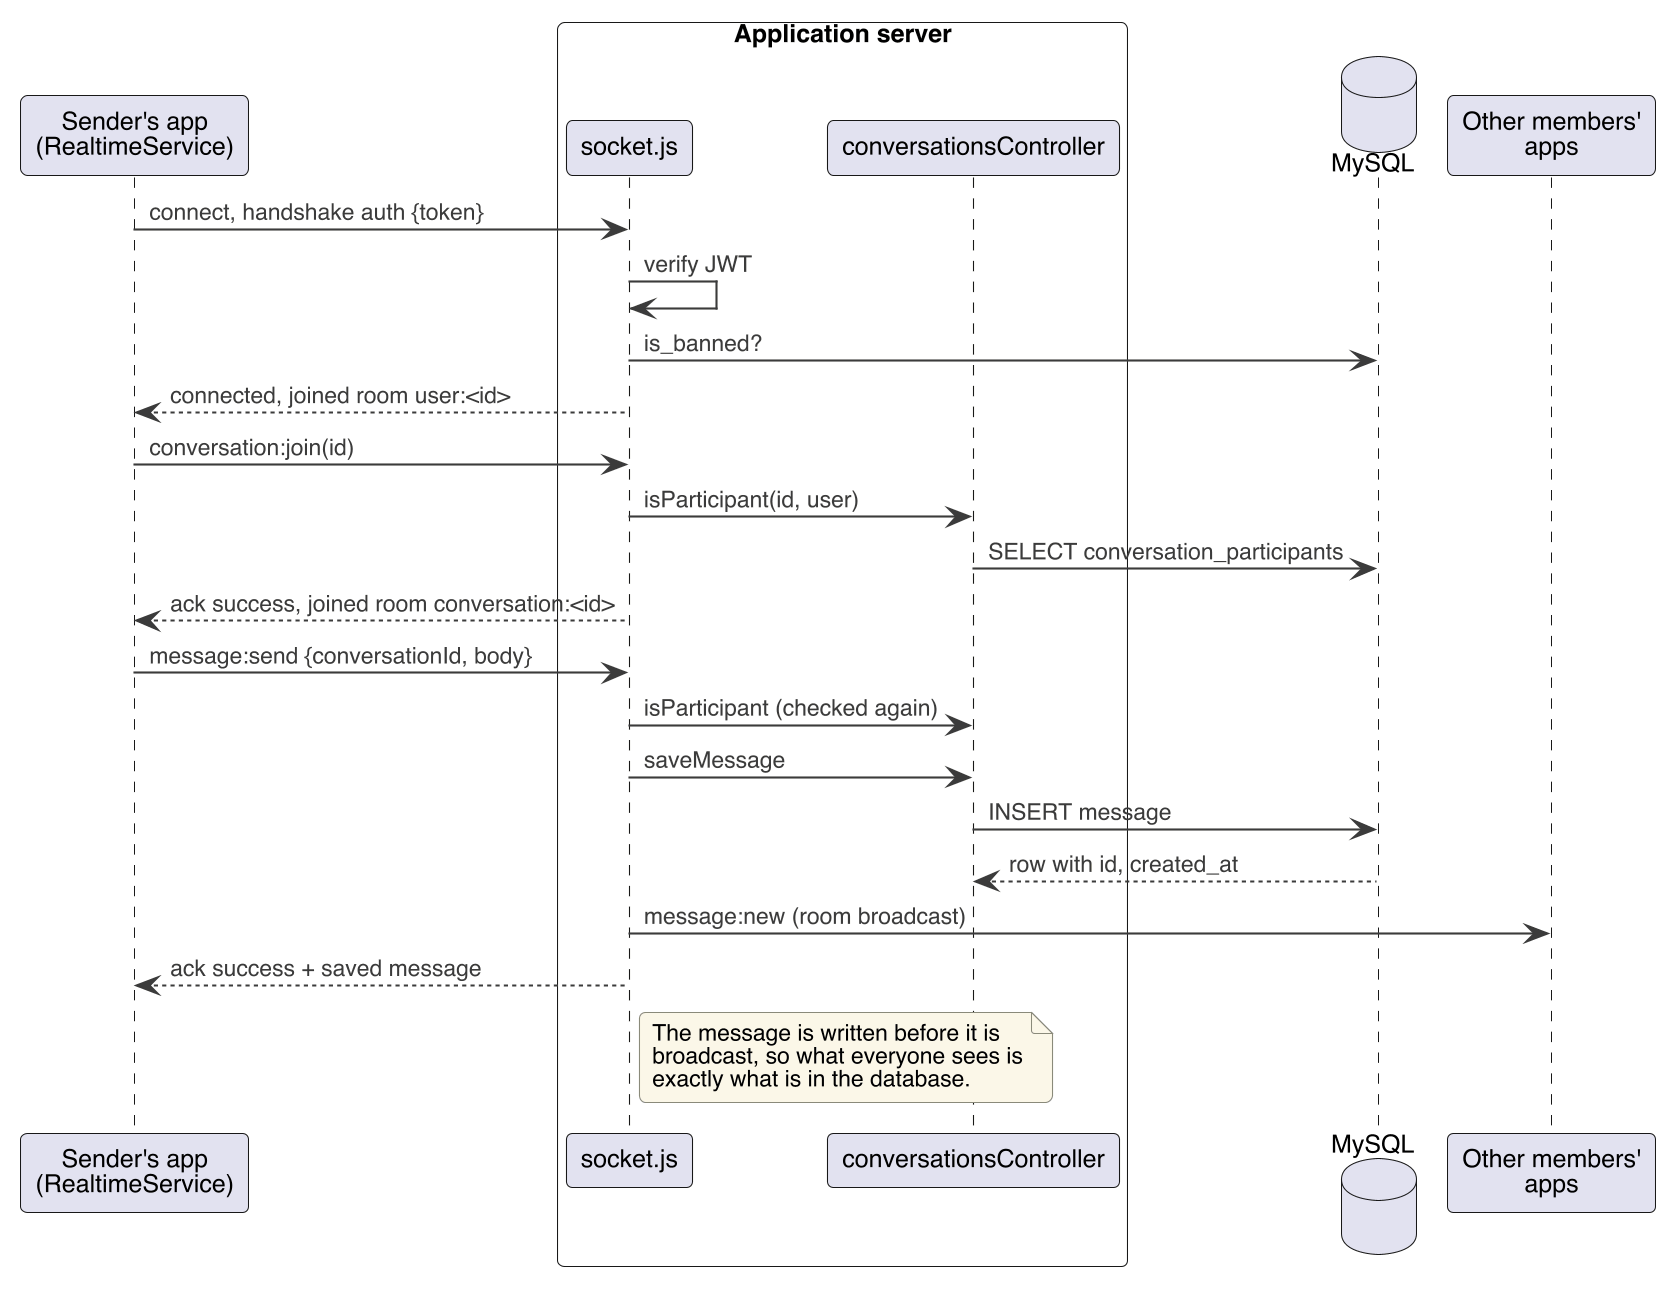
\includegraphics[width=0.85\textwidth]{figures/sequence-chat.png}
\caption{Sequence diagram: sending a group chat message}
\label{fig:seqchat}
\end{figure}

\section{Communication Diagram}

Figure~\ref{fig:comm} shows the accept step again as a communication diagram. Where the
sequence diagram is about order in time, this one is about which objects talk to which: the
controller is the only object that writes to the database for the join itself, and it reaches
the guest's phone only through the notifications module and the socket layer, never directly.

\begin{figure}[htbp]
\centering
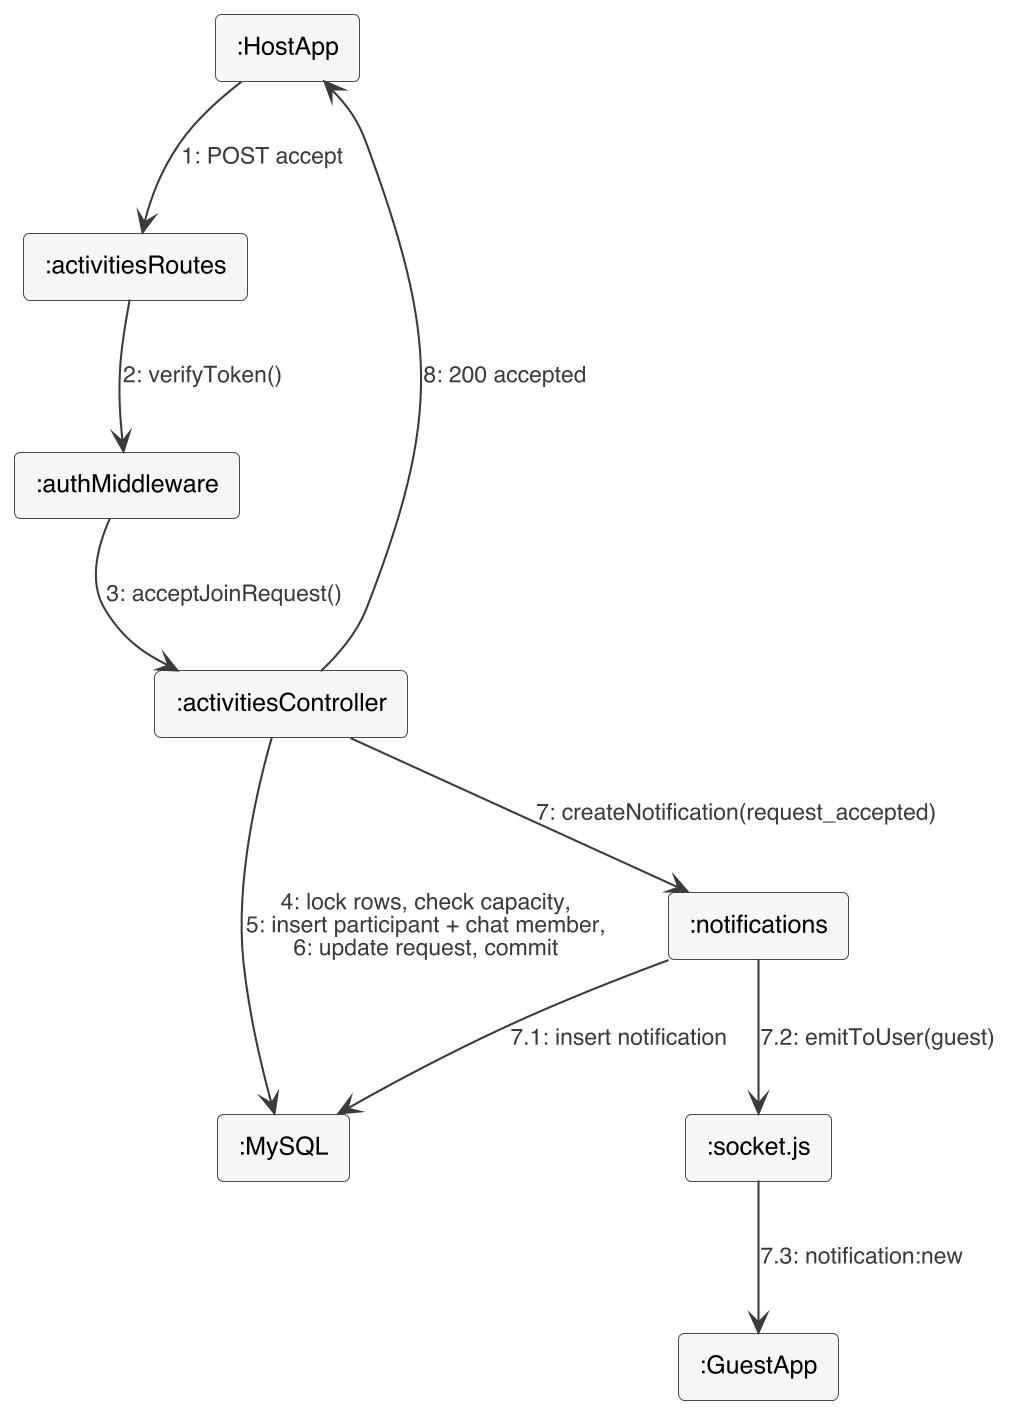
\includegraphics[width=0.55\textwidth]{figures/communication-accept.png}
\caption{Communication diagram: the host accepts a join request}
\label{fig:comm}
\end{figure}

\section{State Diagrams}

Figure~\ref{fig:statereq} has two state machines. A join request has three real states, and
the two self-loops are the rules that matter: accepting into a full activity leaves the request
pending, and asking again after a decline changes nothing. An account starts unverified, and
once active it has a nested ID check state that an admin can also set. Banning is a state of
its own that blocks login, the API and the socket together. Figure~\ref{fig:stateact} is the
life of an activity, where ratings open only in the Finished state.

\begin{figure}[htbp]
\centering
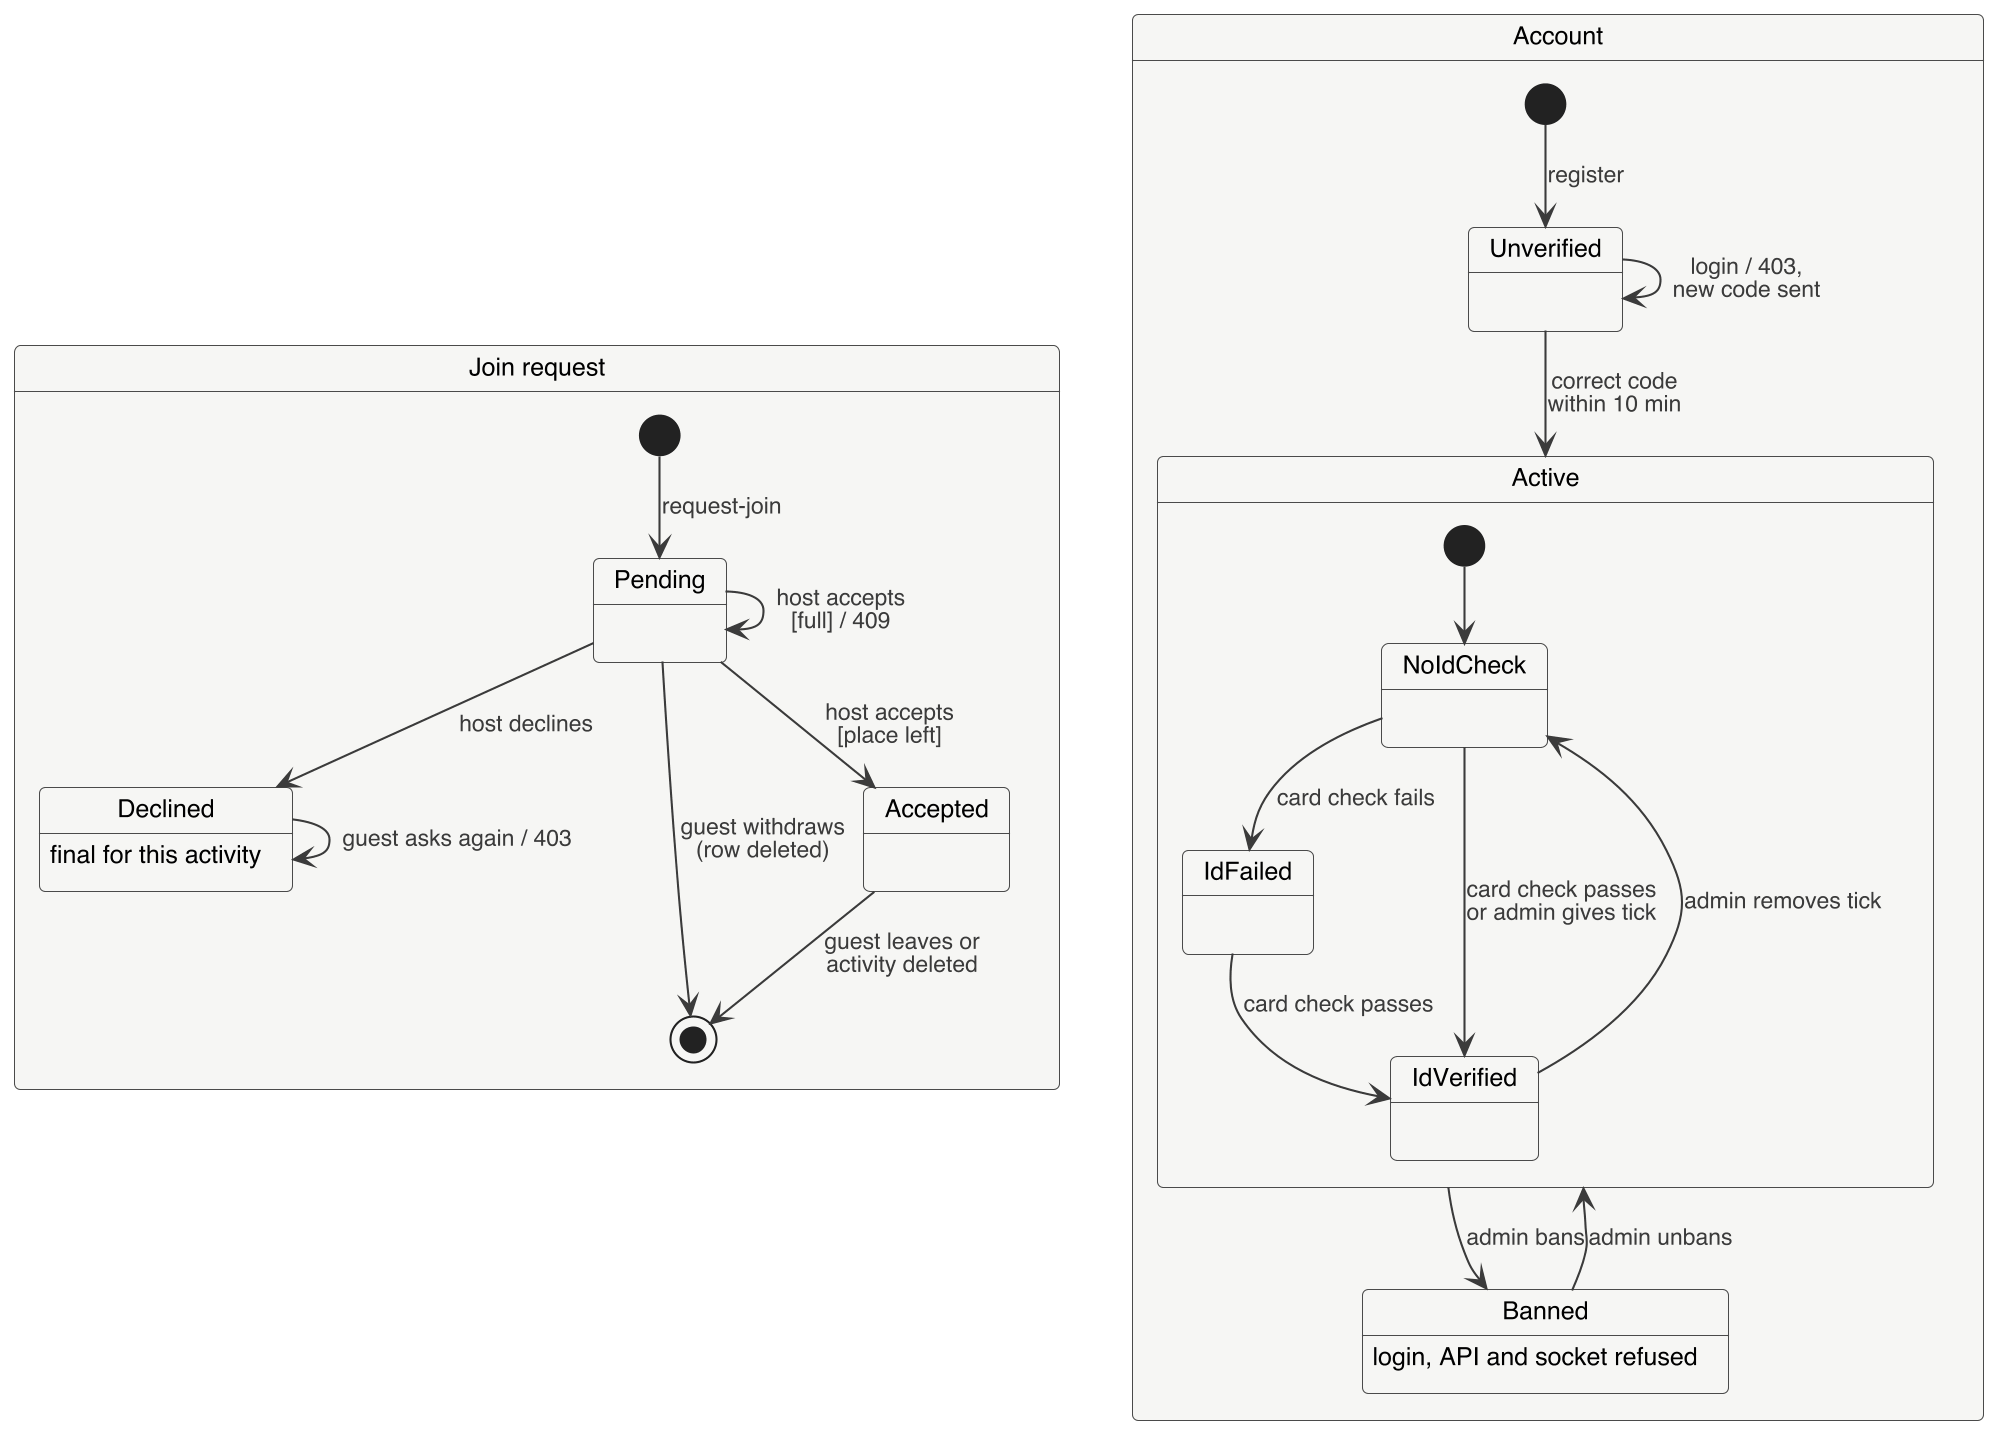
\includegraphics[width=\textwidth]{figures/state-request-account.png}
\caption{State diagrams for a join request and for an account}
\label{fig:statereq}
\end{figure}

\begin{figure}[htbp]
\centering
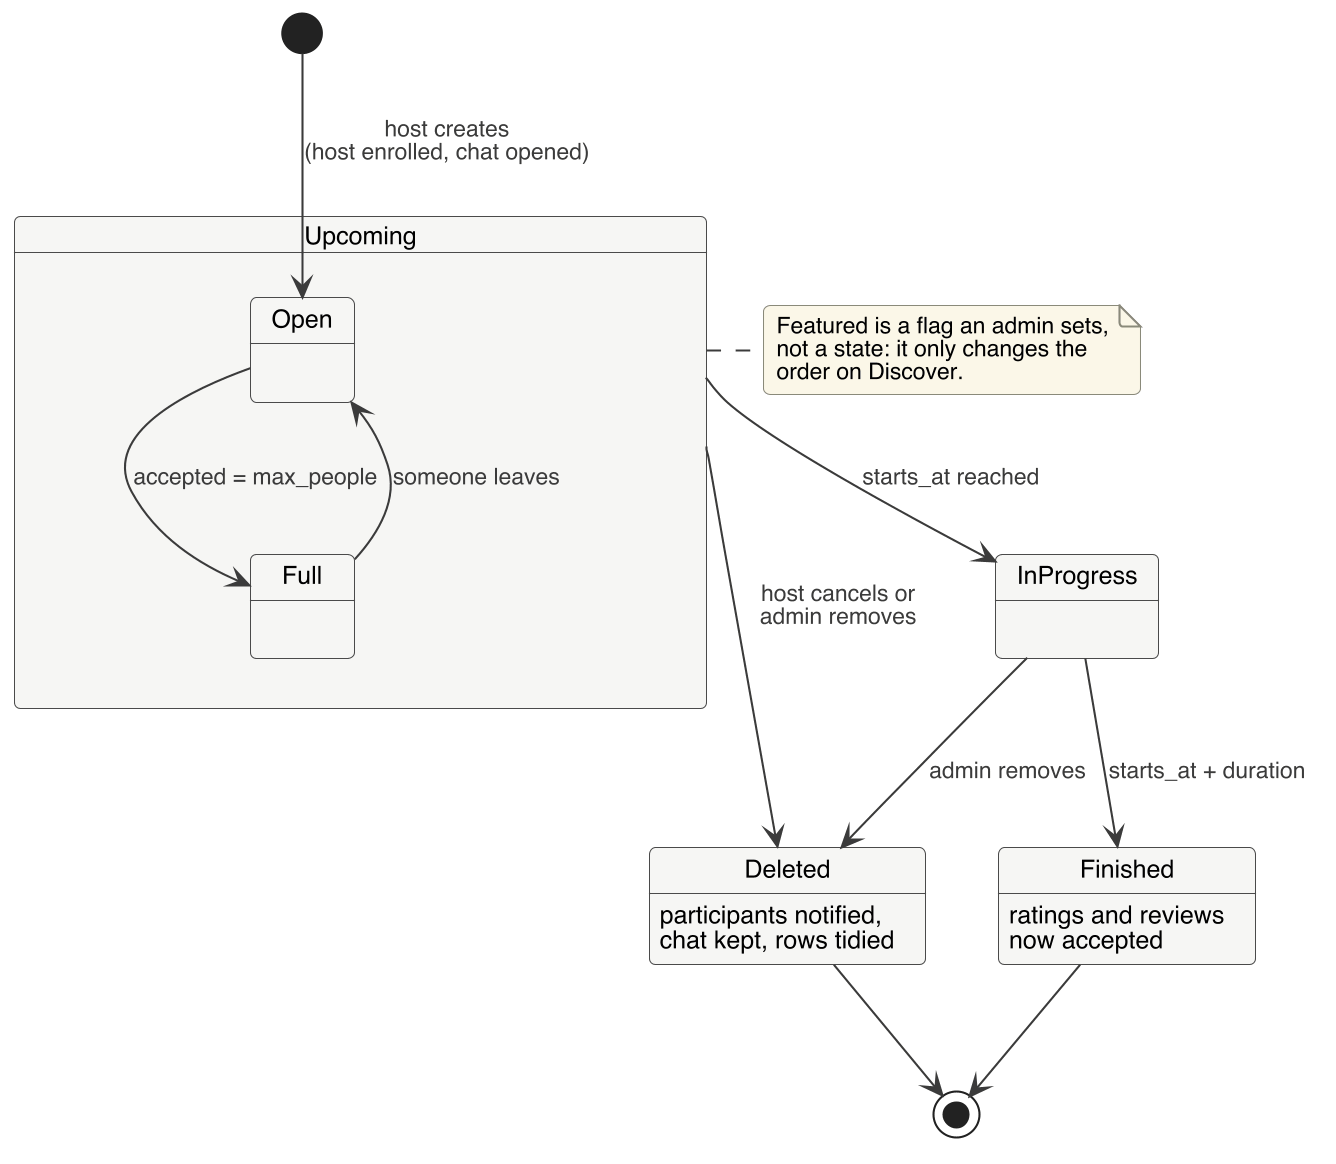
\includegraphics[width=0.75\textwidth]{figures/state-activity.png}
\caption{State diagram for an activity}
\label{fig:stateact}
\end{figure}

\section{Component Diagram}

Figure~\ref{fig:component} shows the software components and their dependencies. The app
reaches the server through exactly two ports, REST and Socket.IO. On the server every
request passes the routers and then either the JWT middleware or the admin guard before a
controller sees it, and only the four adapters talk to anything outside the process apart from
MySQL.

\begin{figure}[htbp]
\centering
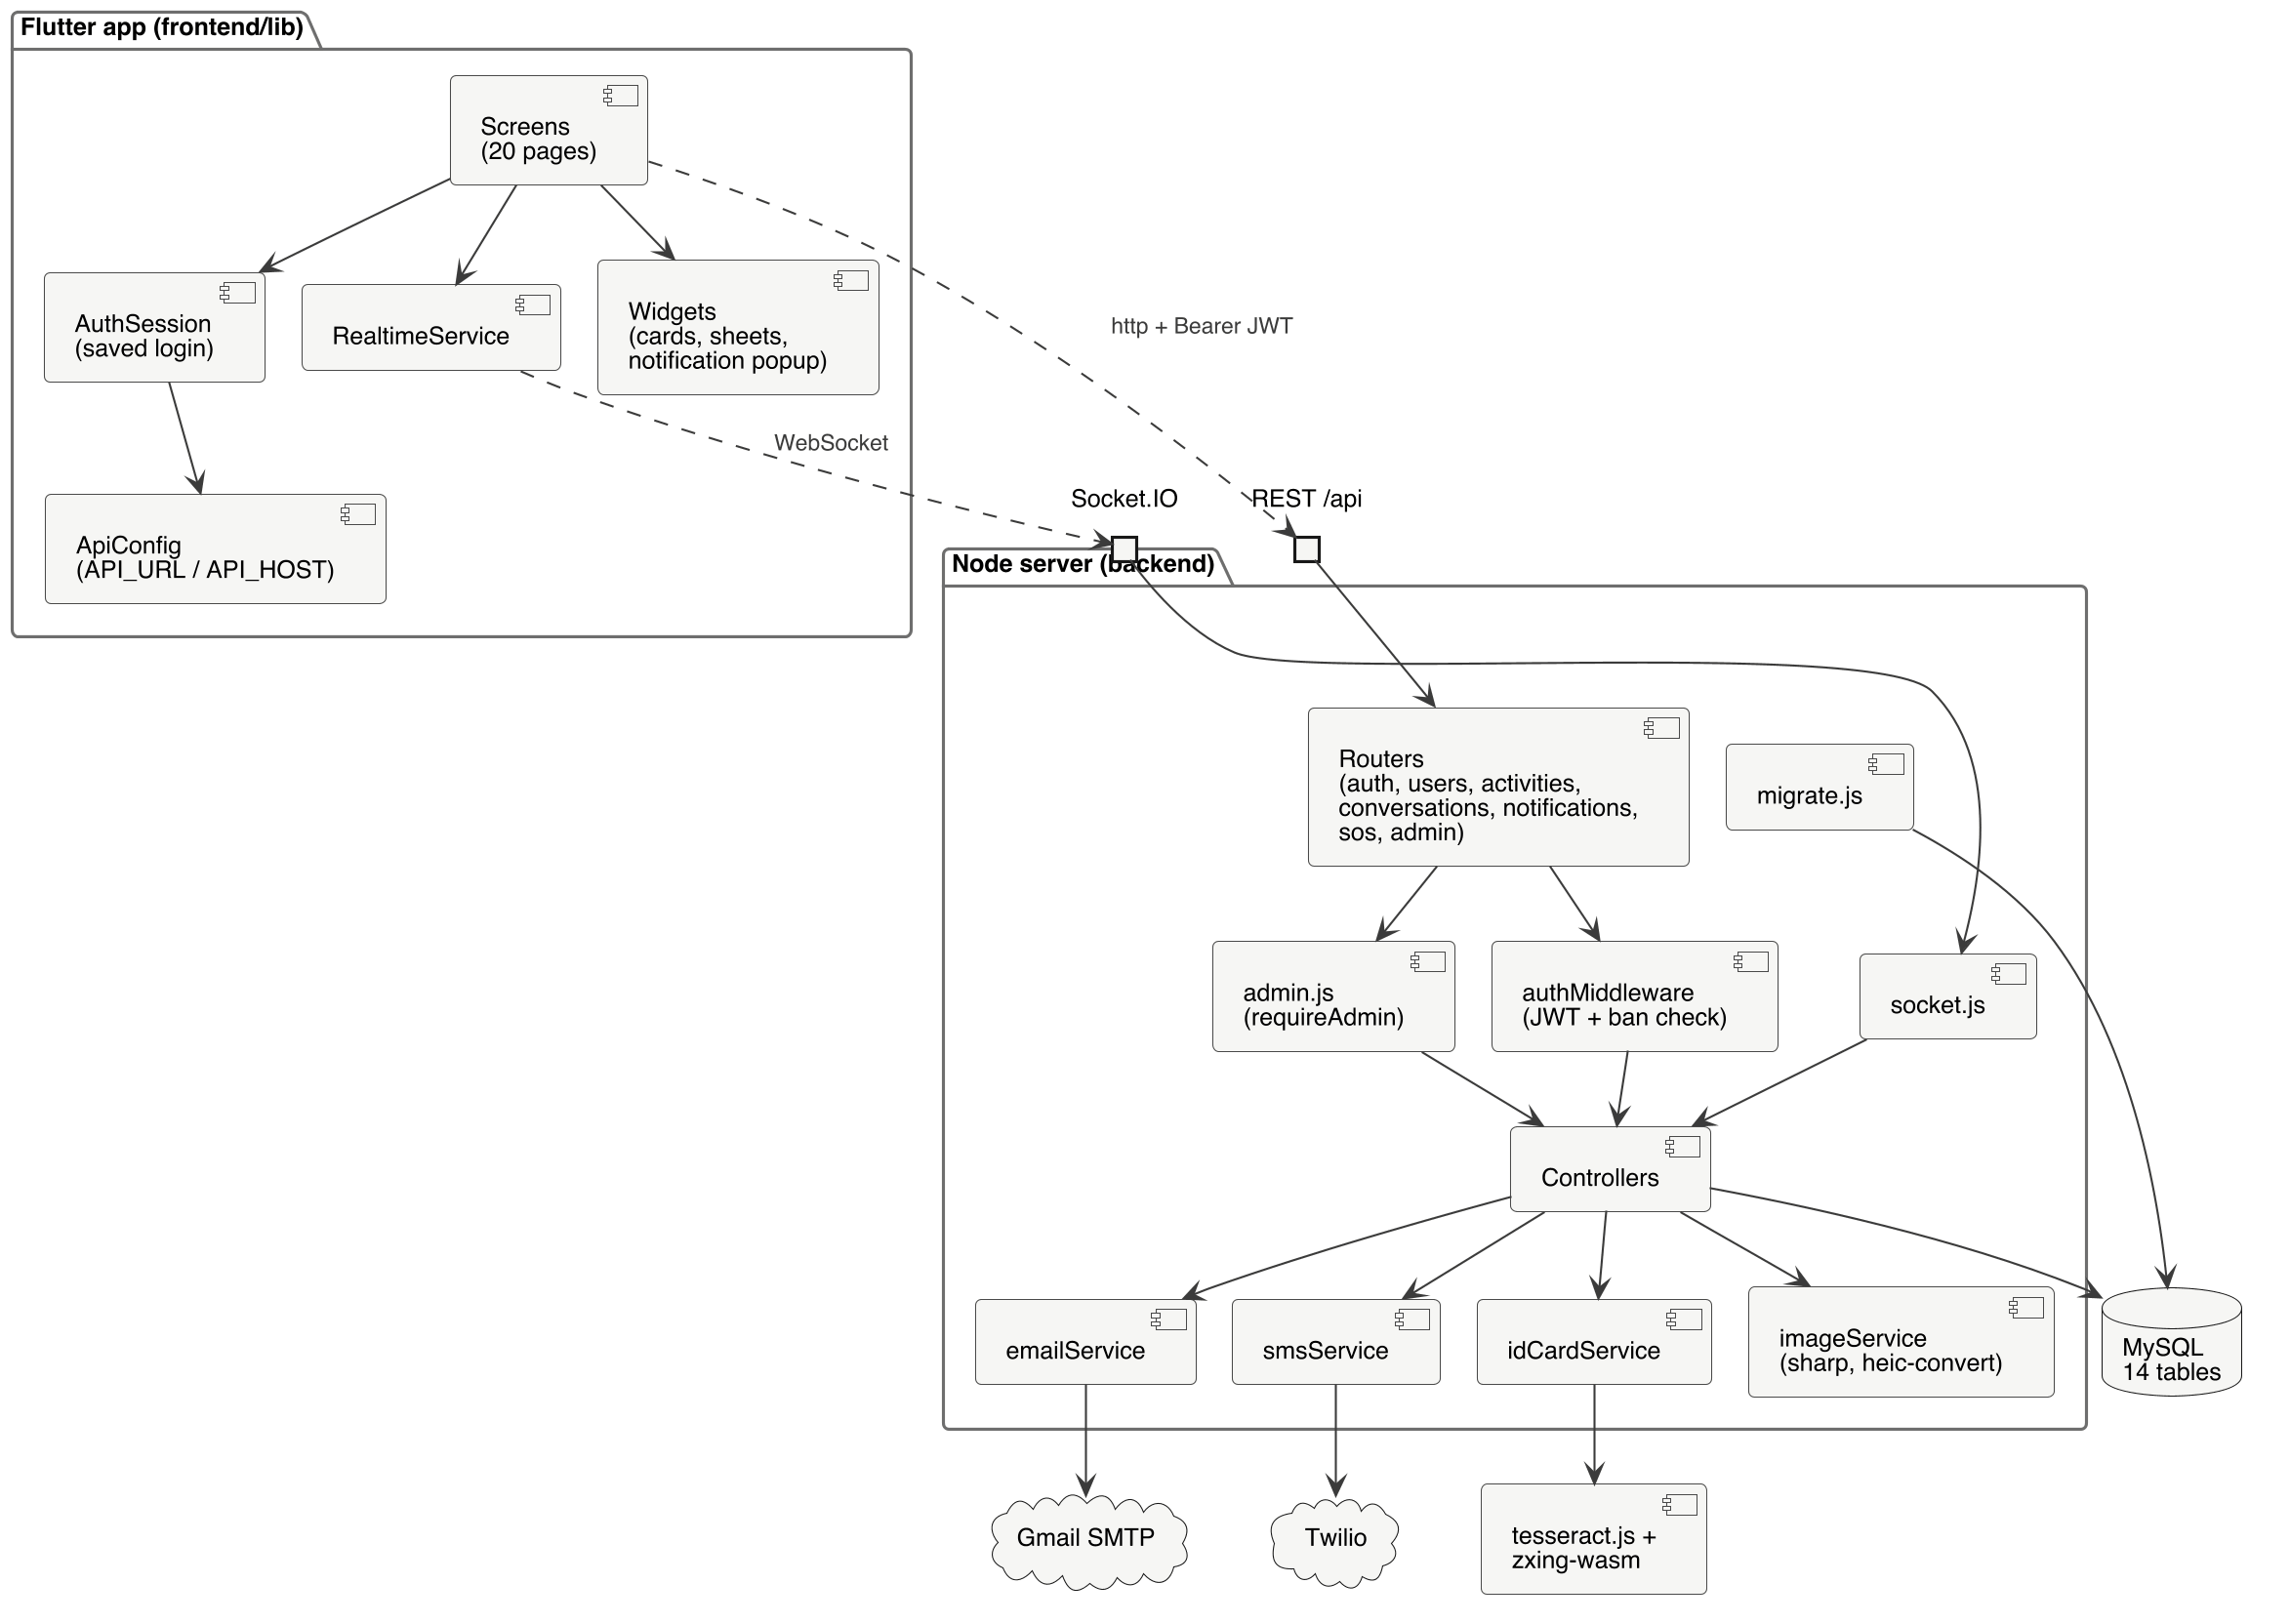
\includegraphics[width=\textwidth]{figures/component.png}
\caption{Component diagram}
\label{fig:component}
\end{figure}

\section{Deployment Diagram}
\label{sec:deploy}

Figure~\ref{fig:deploy} shows where everything runs at the final evaluation. The server,
database and uploaded photos are all on one team laptop, and phones reach it through an ngrok
tunnel on a fixed HTTPS address. This is enough for a demonstration and a small trial. It is
not a production deployment: the service is up only while the laptop is on.

\begin{figure}[htbp]
\centering
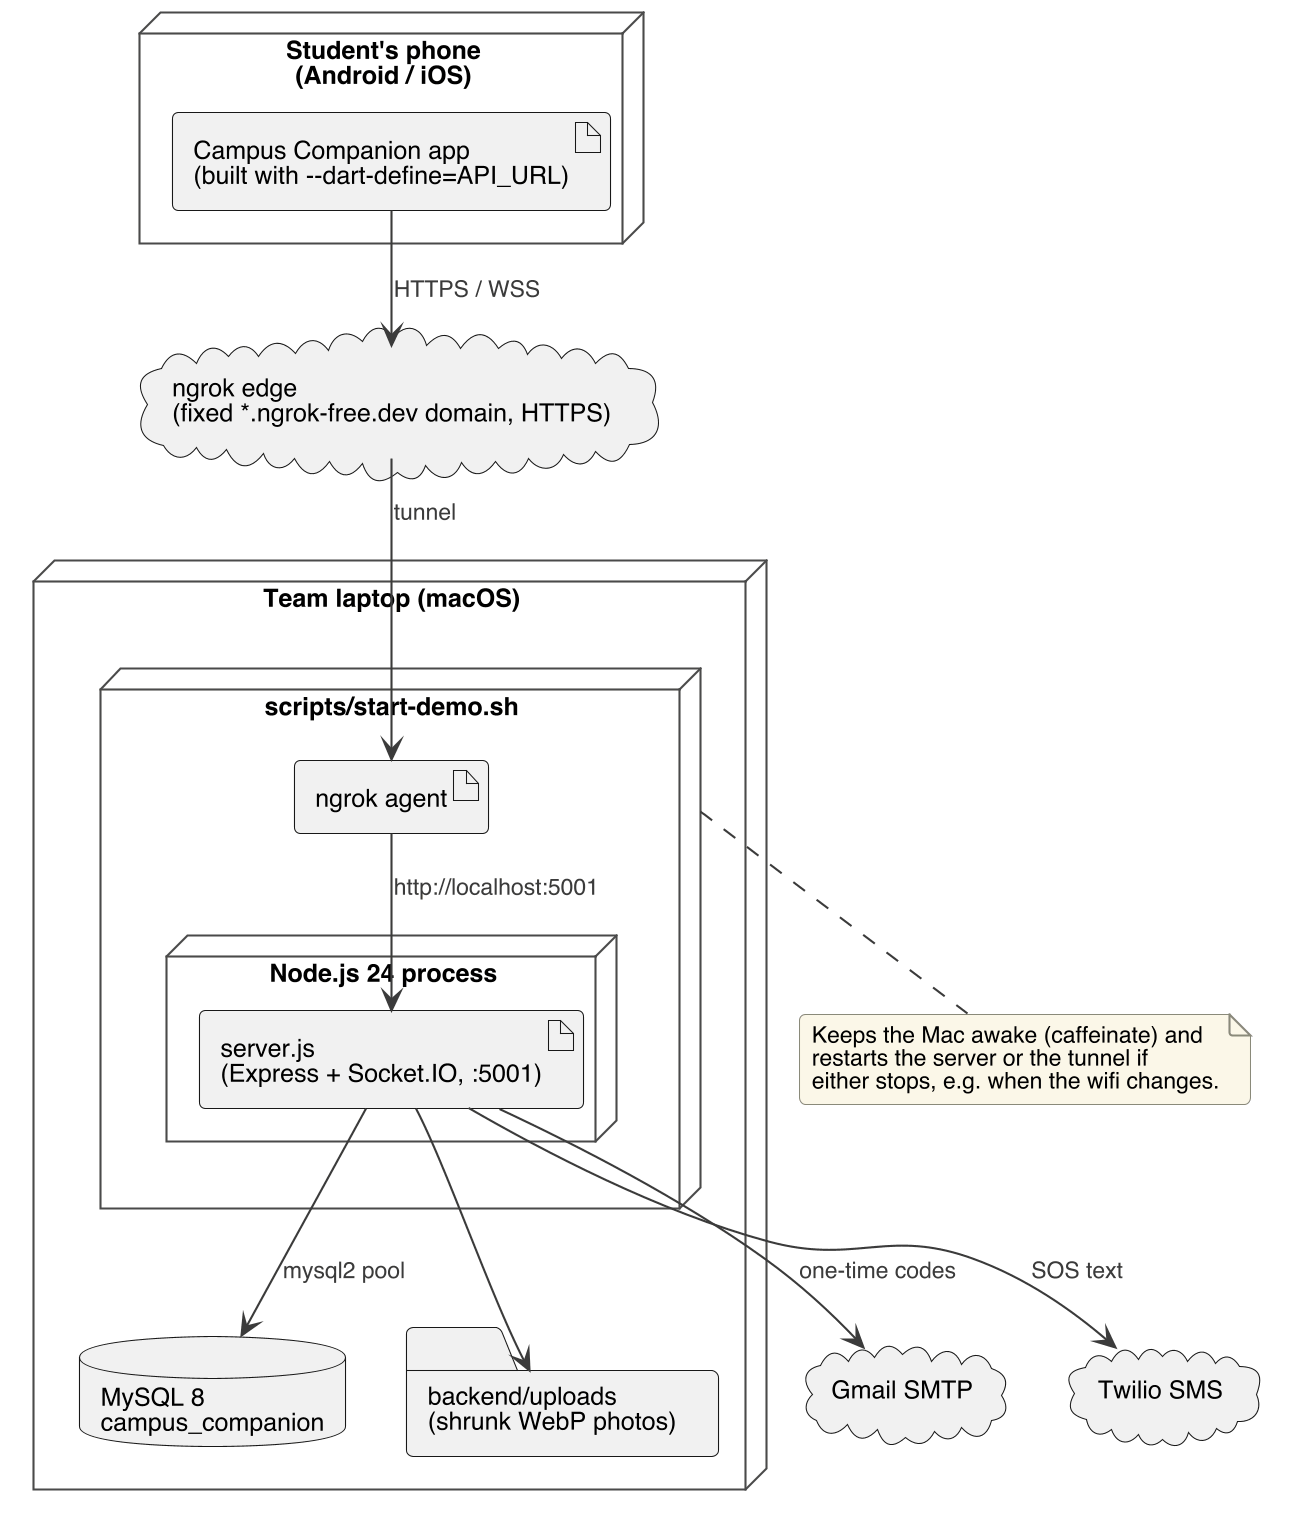
\includegraphics[width=0.75\textwidth]{figures/deployment.png}
\caption{Deployment diagram}
\label{fig:deploy}
\end{figure}


% ===== CHAPTER 8: CONCLUSION =====

\chapter{Conclusion}
\label{ch:conclusion}

\section{Summary of Work}

Over the semester the project went from an empty repository to a working two-part system: a
twenty-screen Flutter application and a Node.js server over MySQL, exposing 44 REST endpoints
and a real-time channel for chat and notifications. A student can register with an
institutional address and prove it with a one-time code, check their account against their
Thapar ID card, post an activity or a multi-day event, find what others have posted, ask to
join and be accepted or refused by the host, talk to the group in a chat that exists from the
moment the activity does, sign up for activities and teams inside an event, and rate and review
the people they went with. Admins can ban, remove content and feature activities. The app keeps
a student logged in, and phones on any network reach the server through a fixed HTTPS address.

Of the six objectives, four are complete and two are not. The SOS path works on the server and
is tested, but the button in the app was never connected to the phone's location. The pilot
that would have measured real use was not run. In their place, Chapter~\ref{ch:testing} adds a
suite of 48 automated tests, all passing, and Chapter~\ref{ch:results} measures the system's
speed and how it scales.

\section{Key Findings}

\begin{itemize}
  \item \textbf{The approval step is the product.} The single decision that separates
        Campus Companion from a group chat is that joining is a request the host answers,
        not an action a stranger takes. Everything else the system does, the verified
        identity, the ratings and reviews, the emergency contact, exists to give that host
        enough information to answer well.

  \item \textbf{Measure the idea before trusting it.} Face matching looked like the obvious
        way to verify a student, and the feasibility study assumed it. A single test with a
        real card, where the owner scored 22\%, showed it could not work with the photographs
        Thapar prints. Reading the text and barcode, which the study never considered, works.
        The same thing happened with performance: the rating subquery was expected to be the
        bottleneck, and measurement showed the response size was.

  \item \textbf{The interesting bugs lived between correct pieces of code.} The capacity check
        and the insert were each correct, and an activity could still overfill. The chat screen
        and the notification service each worked, and sharing one socket broke both. The
        upload check and the HEIC conversion were each correct, and iPhone photos were still
        refused. None of these shows up reading one file at a time.

  \item \textbf{A test can lie.} Two of the new tests passed at first without testing what
        their names said, one because the request failed for an earlier reason. A passing test
        is only worth something if it would fail when the feature breaks.

  \item \textbf{Real phones find problems simulators never do.} Android release builds with
        no internet permission, campus wifi that isolates devices, and an iPhone swipe back to
        the login page were all invisible until the app went onto other students' phones.
\end{itemize}

\section{Future Work and Recommendations}

\begin{enumerate}
  \item Connect the SOS control to the phone's location, with the permission prompt and a
        confirmation step, and complete Objective~5. The server side is already done.
  \item Run the two-week pilot with one batch and report time to a confirmed companion,
        acceptance rate, fill rate and rating coverage from the database.
  \item Paginate Discover with a keyset cursor on \texttt{starts\_at}; at 4{,}000 activities
        each visit currently sends 1.7~MB.
  \item Move the server off the laptop onto a hosted machine, and uploaded photos onto object
        storage.
  \item Let students report and block one another, the half of the study's moderation
        proposal that is still missing.
  \item Connect the activity search box on Discover to the \texttt{search} parameter the
        server already accepts, and show the rating count beside the average on activity cards.
  \item Run both test suites automatically on every push.
\end{enumerate}

\section{Final Remarks}

At mid-semester this report said the second half would add no new subsystem. That turned out
to be wrong: ID card checking, events, moderation and live notifications are all new, and each
came from putting the app in front of people and seeing what they asked for. What the second
half did not do is the work that was planned for it first, wiring SOS to the phone and running
the pilot. Those two are listed at the top of the future work on purpose.

The test suite is the part most likely to outlast this semester. It encodes, in 29 server
cases, the rules the system depends on: who may join, who may see what, and what happens when
two people want the last place at once. Anyone who changes the code after this report can now
find out in under a minute whether those rules still hold.


% ===== CHAPTER 9: PROJECT JOURNAL =====

\chapter{Project Journal}
\label{ch:journal}

This chapter records the team's work in date order, with the errors met along the way and
how they were fixed. All four members worked on the application itself, across every part
of it. Each member also led one area, shown in Table~\ref{tab:roles}.

The code was written together but committed from Aryan Vasdev's laptop, which also ran the
server and the database. That is why almost every commit in the repository carries his name;
the commit author shows whose machine the work was saved from, not who did it. The
development log in Section~\ref{sec:devlog} is therefore credited to the team. The sections
after it record what each member led.

\begin{table}[H]
\centering
\begin{tabular}{|L{3.2cm}|L{4.0cm}|L{4.3cm}|}
\hline
\textbf{Member} & \textbf{Led} & \textbf{Also worked on} \\
\hline
Aryan Vasdev & Server, database and bringing the parts together & All four parts of the app \\
\hline
Ishaan Sharma & Starter app, sign-in screens, theme and navigation & All four parts of the app \\
\hline
Saumya Singh & Proposal, feasibility study and UML models & All four parts of the app \\
\hline
Shraney Sharma & Testing & All four parts of the app \\
\hline
\end{tabular}
\caption{Who led what. The four parts of the app are accounts and ID checking; hosting,
joining and events; chat, notifications and reviews; and moderation and running the app on
phones.}
\label{tab:roles}
\end{table}

Entries taken from version control carry the date and time of the commit, from the team's
local repository or from the course repository on GitHub. Work that never went through a
commit, such as writing, drawing and manual testing, is dated by the milestone it was
delivered for.

% Break the page before a member's section when fewer than about ten lines are
% left, so a heading is never stranded above an empty page bottom.
\newcommand{\memberbreak}{\par\vspace{0pt plus 10\baselineskip}\penalty-250\vspace{0pt plus -10\baselineskip}}

\newcommand{\jhead}{%
\hline
\textbf{When} & \textbf{Work done} & \textbf{Errors met, and the fix or improvement} \\
\hline}

% ------------------------------------------------------------------
\section{Team Development Log}
\label{sec:devlog}

The whole team worked on the entries below. Dates and times are those of the commits.

\begin{longtable}{|L{1.6cm}|L{4.2cm}|L{5.2cm}|}
\jhead
\endfirsthead
\jhead
\endhead
\hline
\endfoot
30 Aug & First full commit of the working app: sign-up with one-time codes, hosting,
join requests with host approval, group chat over Socket.IO, ratings, notifications and the
SOS server path. &
Two accepts could overfill an activity because the capacity check and the insert were
separate statements; both moved into one transaction with \texttt{FOR UPDATE} locks. \\
\hline
1 Sep, 04:22 & Forgot-password flow on the same one-time code system. &
A sign-up code could have been replayed to reset a password; codes now carry a
\texttt{purpose}, and the reset endpoint gives the same answer whether or not the address
exists. \\
\hline
1 Sep, 04:34--04:56 & Gender required at sign-up; app pointed at the laptop's new address. &
The app had the laptop's old wifi address hard-coded and could not connect. \\
\hline
1 Sep, 04:56--05:22 & HEIC and HEIF photos converted to JPEG on the server. &
iPhone photos were refused outright. Converting them was not enough on its own: the app
was sending them with no content type, so the upload filter rejected them first. Fixed in a
second commit. \\
\hline
1 Sep, 05:22--05:33 & Emergency contact moved to its own page; show/hide on the password
field. &
Inside Edit Profile the emergency contact read as one more optional field. \\
\hline
18 Sep, 22:27--22:56 & Assembled the mid-semester report in LaTeX; one shared category list
for the host form and Discover. &
The host form offered a ``More\ldots'' chip that posted ``More\ldots'' as a category, which
Discover could not show; found while checking the report against the code. The server now
refuses any category outside the list, and a unit test checks every category has a chip. \\
\hline
19 Nov, 06:46--07:01 & Live notifications over Socket.IO, reviews with tags, public
profiles, teams, and a first ID check by face matching. & --- \\
\hline
19 Nov, 07:26 & App made to work from other students' phones. &
Android release builds had no internet permission and blocked plain HTTP; iOS needed a
local-network permission. All three added. \\
\hline
19 Nov, 09:42 & App can be pointed at a full server address such as a tunnel. &
Campus wifi isolates devices, so phones could not reach the laptop even on the same network. \\
\hline
19 Nov, 10:02 & ID card checked by OCR and barcode instead of faces. &
Face matching scored the real owner of a card at 22\%, so it could not tell people apart.
Replaced with the four-step card check; about 100~MB of TensorFlow dependencies dropped. \\
\hline
19 Nov, 10:14--10:22 & Categories renamed; host form inputs reworked; date and time merged
into one field. &
The $-$ and $+$ buttons had 22-point margins that squeezed the number between them to
nothing when two sat side by side. Margins removed, and a widget test checks the digits fit. \\
\hline
19 Nov, 10:33--10:58 & Events with activities inside them, multi-day events, team activities,
a real Settings page, and the new app icon. &
The duration picker stopped at 12 hours, too short for a three-day fest; events now take an
end date instead. \\
\hline
19 Nov, 11:01 & Navigation after login. &
The iOS back swipe slid from anywhere in the app back to the filled-in login page. Login now
replaces the whole navigation stack. \\
\hline
19 Nov, 14:07--14:28 & Host chooser colours, team setup as teams $\times$ players, and the
one-command start script with a permanent ngrok address. & --- \\
\hline
19 Nov, 14:35 & Removed the in-app setting for the server address. &
Anyone holding the phone could have pointed the app at their own server and collected the
next login. With a permanent address the setting was no longer needed. \\
\hline
19 Nov, 14:42--14:47 & Admin moderation (ban, remove, tick, feature); app named ``Campus
Companion'' on Android. & --- \\
\hline
19 Nov, 15:04 & Chat fix. &
New messages only appeared after reopening a chat, because the chat screen was handed the
notification socket, which was already connected and so never joined the chat room. Chat and
notifications now use separate connections. \\
\hline
19 Nov, 15:08 & Login kept in secure storage across restarts. &
Every restart meant logging in again. \\
\hline
19 Nov, 15:13--15:18 & Group chat button on the activity page; photos shrunk and cached. &
A phone avatar of 423~KB now uploads as 39~KB, which matters on mobile data and the tunnel's
monthly allowance. \\
\hline
20 Nov, 06:13 & Made \texttt{schema.sql} work on a fresh database. &
Setting up the test database showed the script had never run on a clean MySQL install. \\
\hline
20 Nov, 06:16--06:35 & Server test suite and the final report's figures. &
Two tests were fixed after they were found to pass without testing what they claimed
(Chapter~\ref{ch:testing}). \\
\hline
\end{longtable}

% ------------------------------------------------------------------
\clearpage
\section{Aryan Vasdev (1024030549)}

\begin{center}
\begin{tabular}{|L{1.6cm}|L{4.2cm}|L{5.2cm}|}
\jhead
Aug--Nov & Led the server and database: the Express routes and controllers,
the MySQL schema and its transactions, and the Socket.IO layer. &
--- \\
\hline
Aug--Nov & Brought the team's work together on one machine: kept the local
repository, ran the server and database for testing and demos, and pushed to the course
repository. &
--- \\
\hline
18 Sep and 20 Nov & Assembled the mid-semester and final reports in LaTeX from the team's
sections. &
--- \\
\hline
\end{tabular}
\end{center}

% ------------------------------------------------------------------
\section{Ishaan Sharma (1024030553)}

\begin{center}
\begin{tabular}{|L{1.6cm}|L{4.2cm}|L{5.2cm}|}
\jhead
21 Aug (course repo) & Created the starter Flutter application for the team and opened the
first pull request to the course repository; removed the stale code the template had left. &
--- \\
\hline
Before mid-semester & Designed and built the login, sign-up and one-time code screens,
with the red Companion branding on them and the check that only an \texttt{@thapar.edu}
address can be entered. &
--- \\
\hline
Before mid-semester & Set up the app's look: the Material~3 theme in light and dark,
its colours and fonts, and the five-item bottom bar (Home, Discover, Host, Messages,
Profile) that every screen sits in. &
--- \\
\hline
Aug--Nov & Worked with the team on all four parts of the app in the log above
(Table~\ref{tab:roles}). &
--- \\
\hline
\end{tabular}
\end{center}

% ------------------------------------------------------------------
\section{Saumya Singh (1024030554)}

\begin{center}
\begin{tabular}{|L{1.6cm}|L{4.2cm}|L{5.2cm}|}
\jhead
Before implementation & Wrote the project proposal and the feasibility study in
Chapter~2, covering the technical, managerial, economic, financial, cultural, social, safety
and political dimensions, and the go decision. &
--- \\
\hline
Mid-semester (18 Sep) & Drew the use case, class and activity diagrams for the mid-semester
report, with the twenty-one use case scenarios. &
Drawn as one figure, the class model was unreadable at page width, so it was split into a
domain model and an application layer model. \\
\hline
Final evaluation (20 Nov) & Drew the sequence, communication, state, component and deployment
diagrams, and updated the use case and domain class diagrams for ID checks, events and
teams, reviews and the admin role. &
--- \\
\hline
Aug--Nov & Worked with the team on all four parts of the app in the log above
(Table~\ref{tab:roles}). &
--- \\
\hline
\end{tabular}
\end{center}

% ------------------------------------------------------------------
\section{Shraney Sharma (1024030551)}

\begin{center}
\begin{tabular}{|L{1.6cm}|L{4.2cm}|L{5.2cm}|}
\jhead
Before mid-semester & Walked every feature end to end against the real database, on an iOS
device and an Android emulator: sign-up, wrong and expired codes, the resend cooldown,
password reset, hosting, requesting, accepting and declining, full activities, chat across two
devices, ratings and cancelling. &
--- \\
\hline
Before mid-semester & Tested the two risky paths separately: two accepts into one remaining
place, and uploads that were too large, the wrong type, or HEIC from an iPhone. &
--- \\
\hline
Final evaluation (20 Nov) & Test plan and test cases for the final system (Chapter~5):
the levels of testing, the 29 server cases and the system test walk-through with
screenshots. &
--- \\
\hline
Aug--Nov & Worked with the team on all four parts of the app in the log above
(Table~\ref{tab:roles}). &
--- \\
\hline
\end{tabular}
\end{center}



% ===== BIBLIOGRAPHY =====

\printbibliography[heading=bibintoc]

\end{document}
